% FIGURES FOR ENSEMBLE VIRTUAL SPECTROMETRY PAPER
% This file contains detailed specifications for all validation figures

\begin{figure}[htbp]
  \centering
  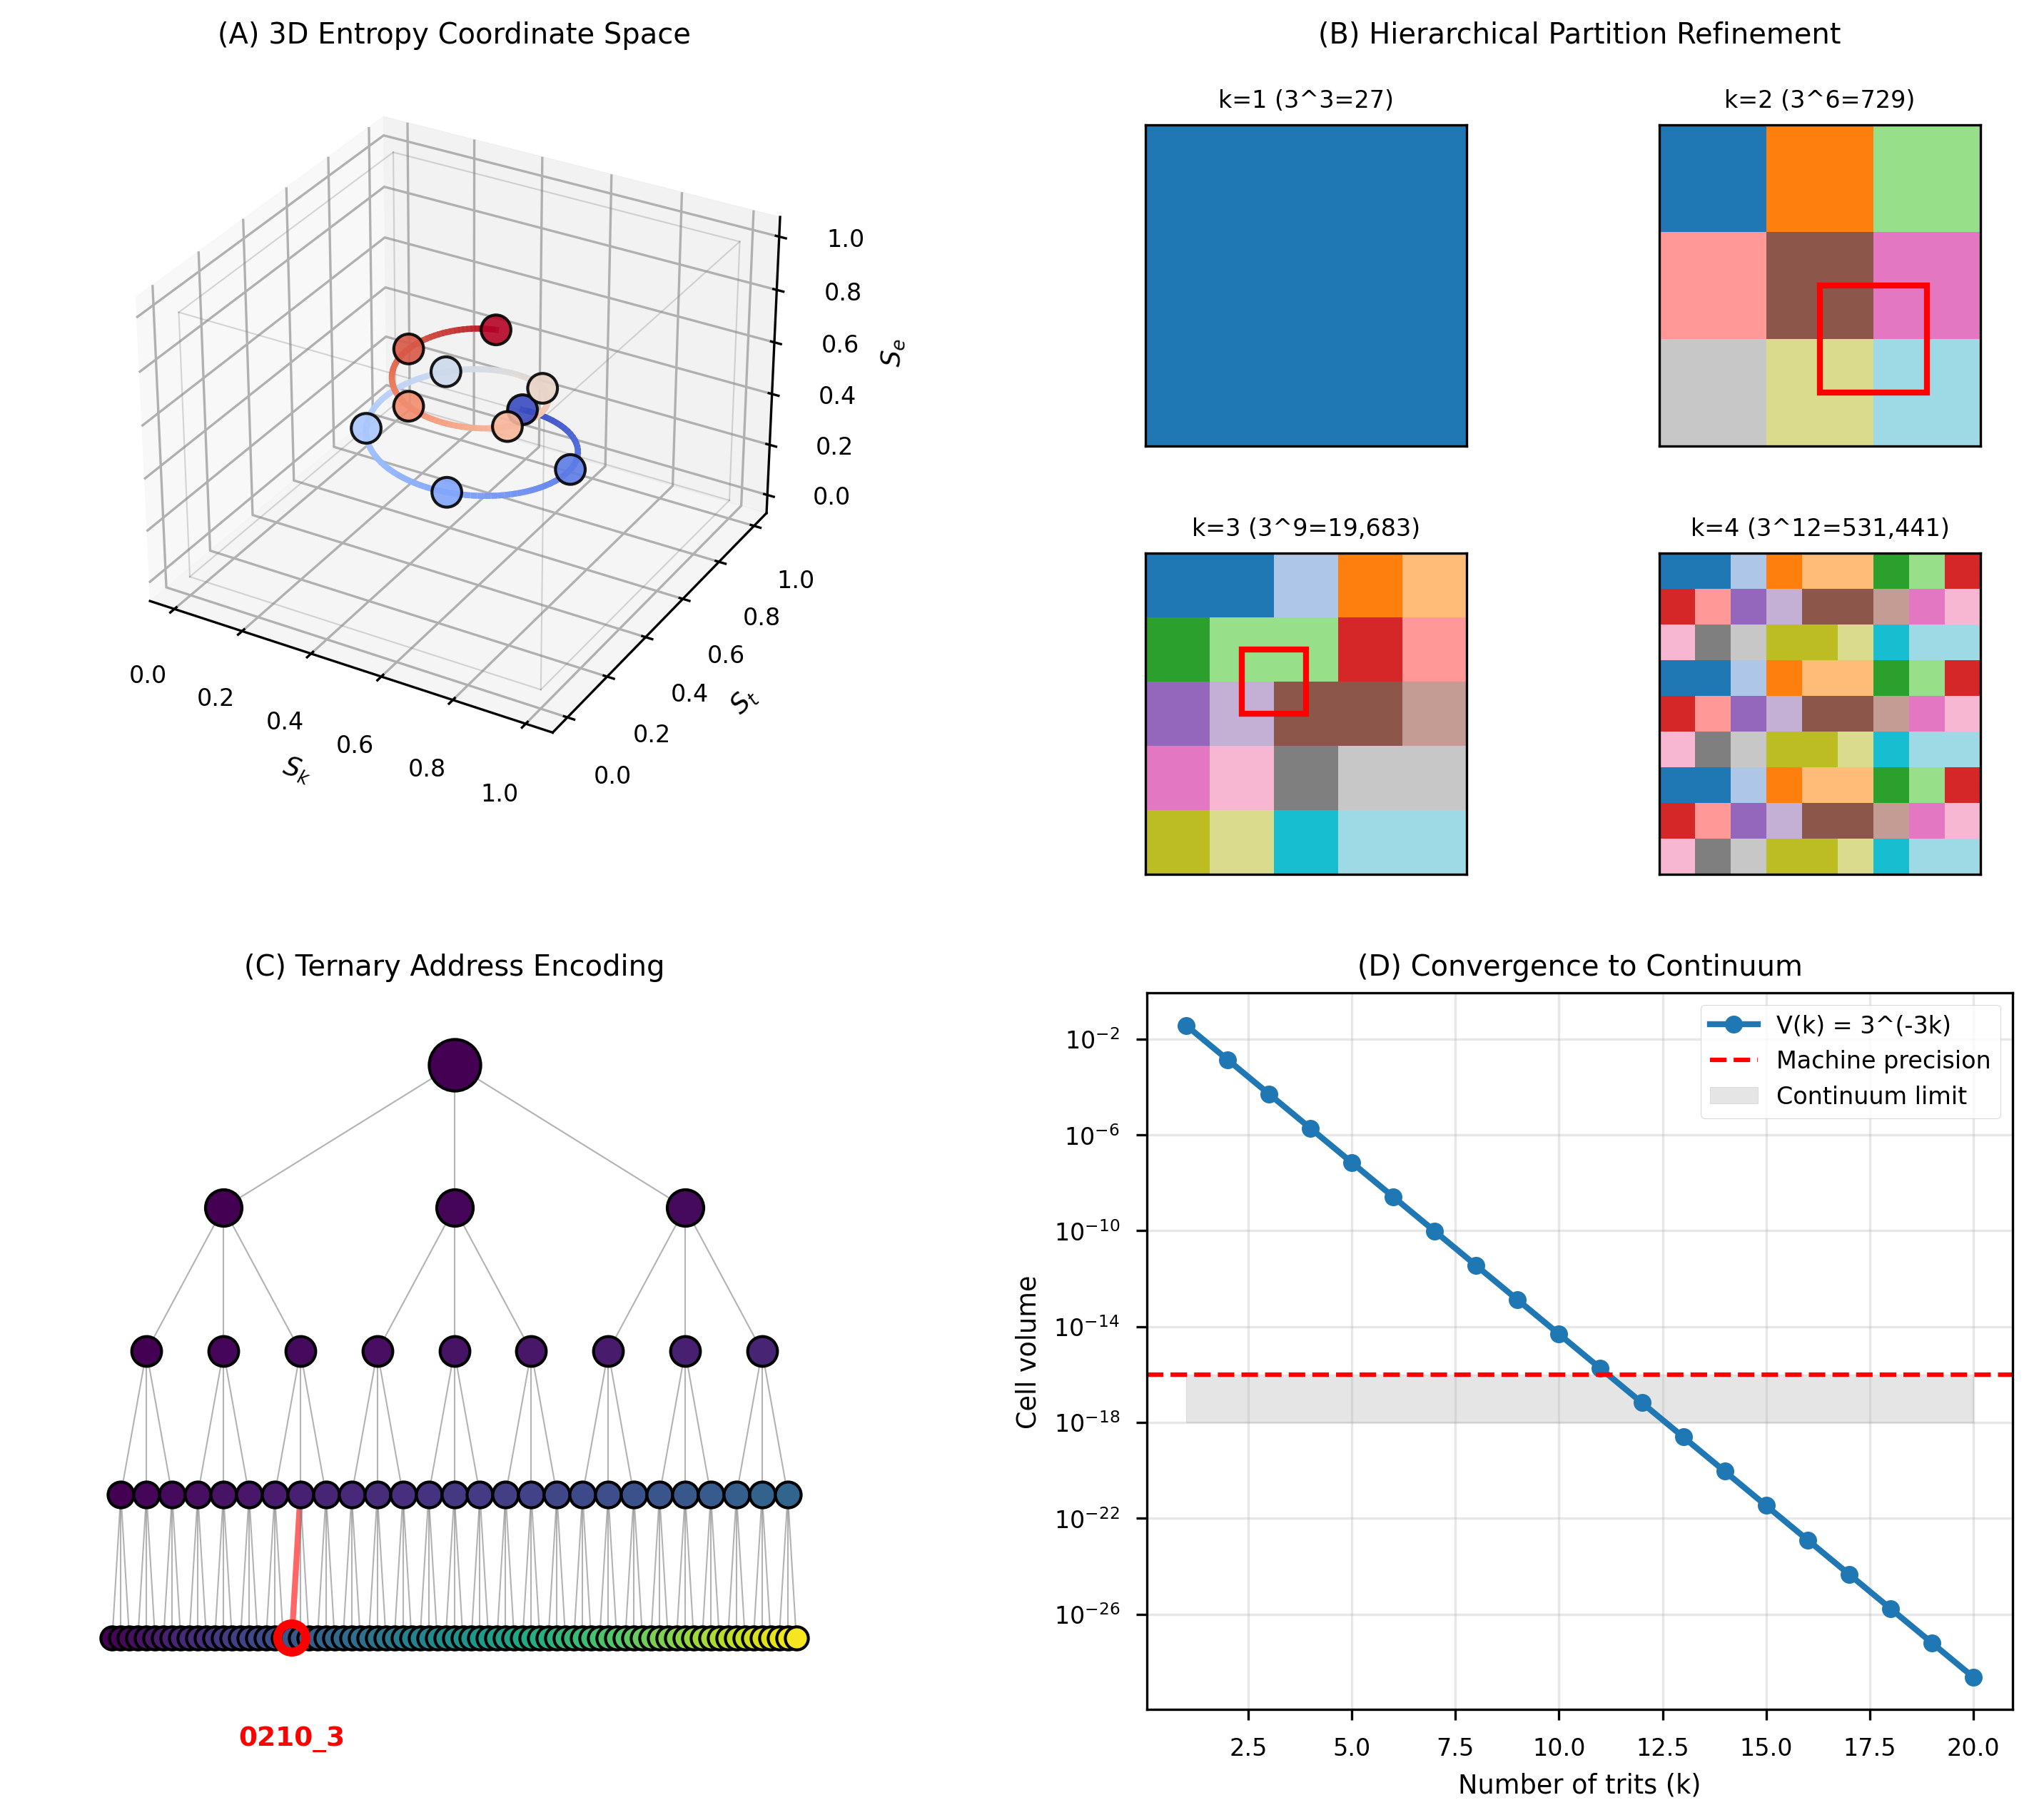
\includegraphics[width=\textwidth]{figures/figure1_ternary_encoding.png}
  \caption{\textbf{Ternary encoding in three-dimensional entropy coordinate space.} 
  (A) Unit cube $$S = [0,1]^3$$ with coordinates $$(S_k, S_t, S_e)$$ showing sample trajectory (blue curve connecting spheres) and discrete categorical states (colored spheres). Wireframe grid illustrates partition structure. 
  (B) Hierarchical partition refinement from $$k=1$$ to $$k=4$$ trits, showing exponential growth in resolution: $$k=1$$ yields $$3^3=27$$ cells, $$k=2$$ yields $$3^6=729$$ cells, $$k=3$$ yields $$3^9=19{,}683$$ cells, and $$k=4$$ yields $$3^{12}=531{,}441$$ cells. Red square highlights example cell refinement sequence. 
  (C) Ternary tree structure encoding cell addresses through hierarchical branching. Each node branches into three children (ternary digits 0, 1, 2). Example address $$0210_3$$ (highlighted in red) traces path from root to terminal node, with final level showing full ternary representation (colored gradient from purple through rainbow to yellow). 
  (D) Cell volume convergence $$V(k) = 3^{-3k}$$ versus number of trits $$k$$, plotted on logarithmic scale. Exponential decay (blue curve with markers) approaches machine precision (red dashed line at $$\sim 10^{-16}$$) around $$k \approx 11$$, entering continuum limit (gray shaded region). Beyond this threshold, discrete cells become indistinguishable from continuous coordinates.}
  \label{fig:ternary_encoding}
  \end{figure}

  \begin{figure}[htbp]
    \centering
    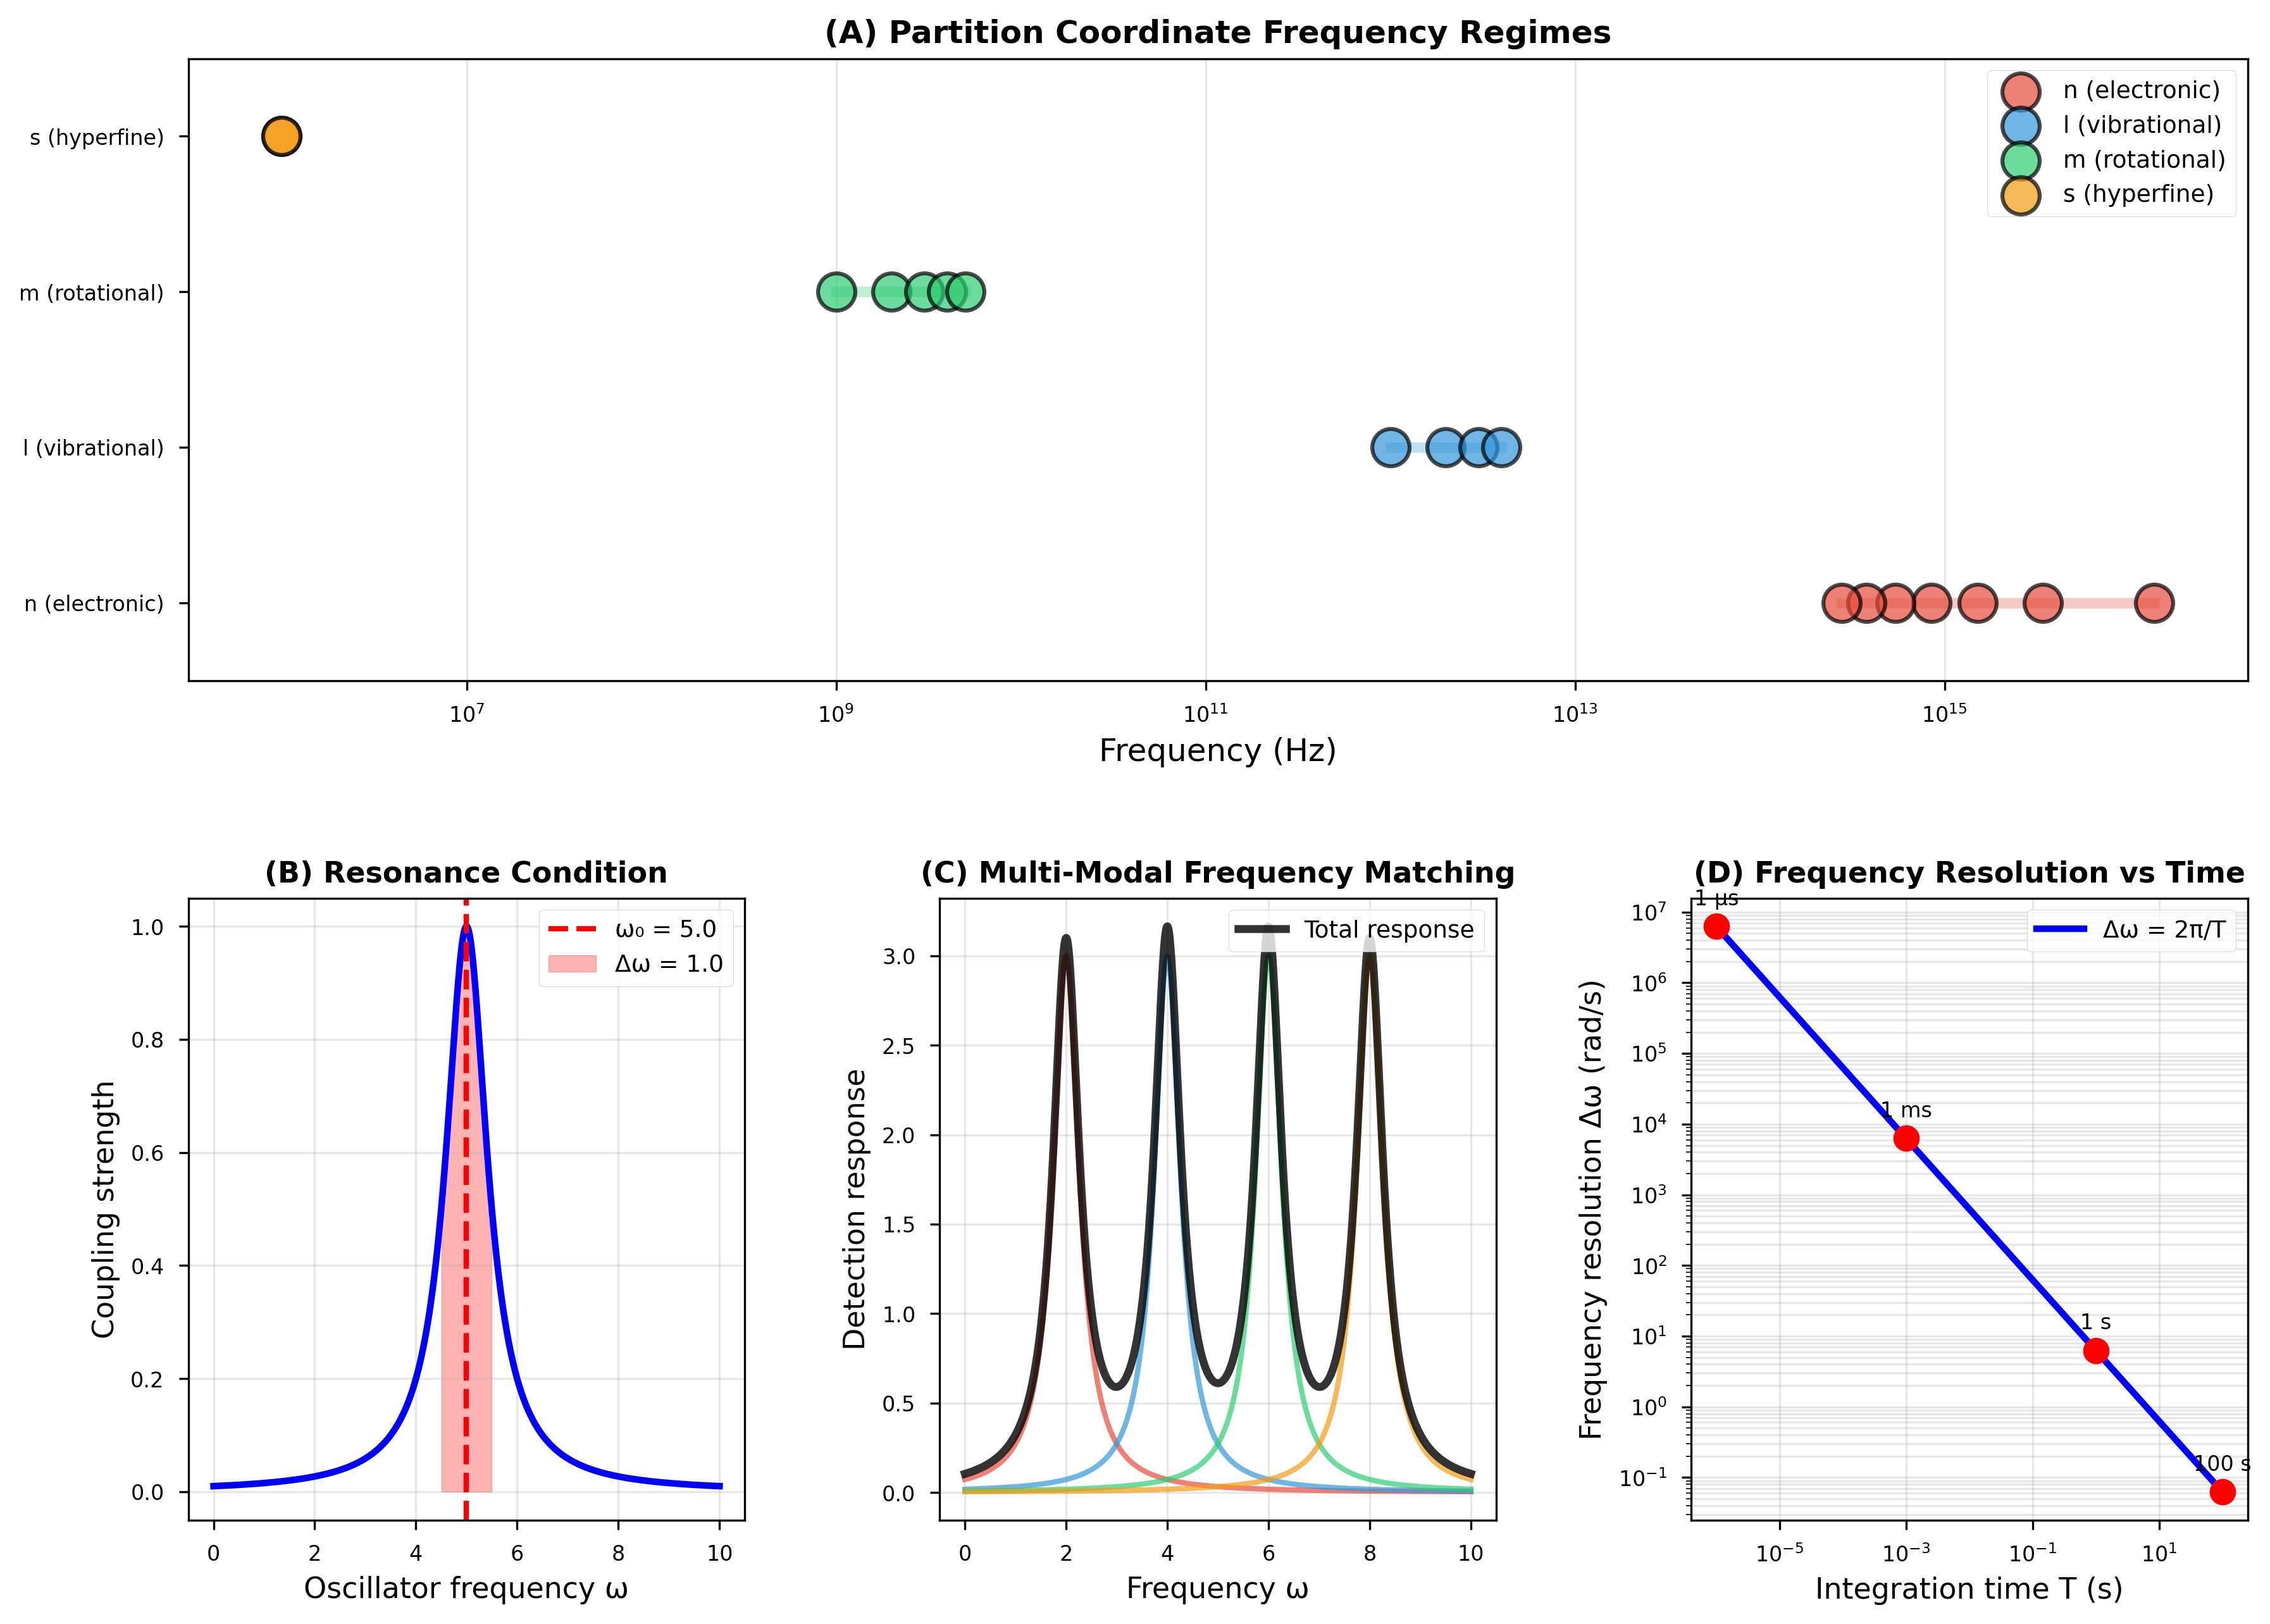
\includegraphics[width=\textwidth]{figures/figure2_frequency_coupling.png}
    \caption{\textbf{Frequency-selective coupling and partition coordinate measurement.} 
    (A) Partition coordinate frequency regimes spanning 15 orders of magnitude. Four distinct frequency bands correspond to quantum numbers: $$n$$ (electronic, red, $$\sim 10^{15}$$ Hz), $$\ell$$ (vibrational, blue, $$\sim 10^{13}$$ Hz), $$m$$ (rotational, green, $$\sim 10^{11}$$ Hz), and $$s$$ (hyperfine, yellow, $$\sim 10^7$$ Hz). Each coordinate occupies well-separated frequency regime, enabling independent measurement through frequency-selective coupling. 
    (B) Resonance condition for frequency-selective coupling. Coupling strength (vertical axis) peaks when oscillator frequency $$\omega$$ matches characteristic frequency $$\omega_0$$. Two bandwidth cases shown: narrow bandwidth $$\Delta\omega = 1.0$$ (red dashed curve) provides high selectivity, wide bandwidth $$\Delta\omega = 5.0$$ (blue solid curve) provides broader coupling. Peak at $$\omega = \omega_0 \approx 5$$ demonstrates resonant enhancement. 
    (C) Multi-modal frequency matching with four independent detection channels. Each colored curve (red, blue, green, yellow) represents frequency-selective aperture centered at different characteristic frequency. Total detection response (black curve) shows combined multi-modal measurement capability. Non-overlapping peaks enable simultaneous independent measurement of all four partition coordinates $$(n, \ell, m, s)$$. 
    (D) Frequency resolution versus integration time, demonstrating fundamental uncertainty relation $$\Delta\omega = 2\pi/T$$. Blue line shows inverse relationship on log-log scale. Red markers indicate characteristic timescales: 1~ms integration yields $$\sim 10^3$$ rad/s resolution, 100~s integration yields $$\sim 10^{-1}$$ rad/s resolution. Gray horizontal lines mark frequency regimes from panel A, showing required integration times for each partition coordinate measurement.}
    \label{fig:frequency_coupling}
    \end{figure}

    \begin{figure}[htbp]
      \centering
      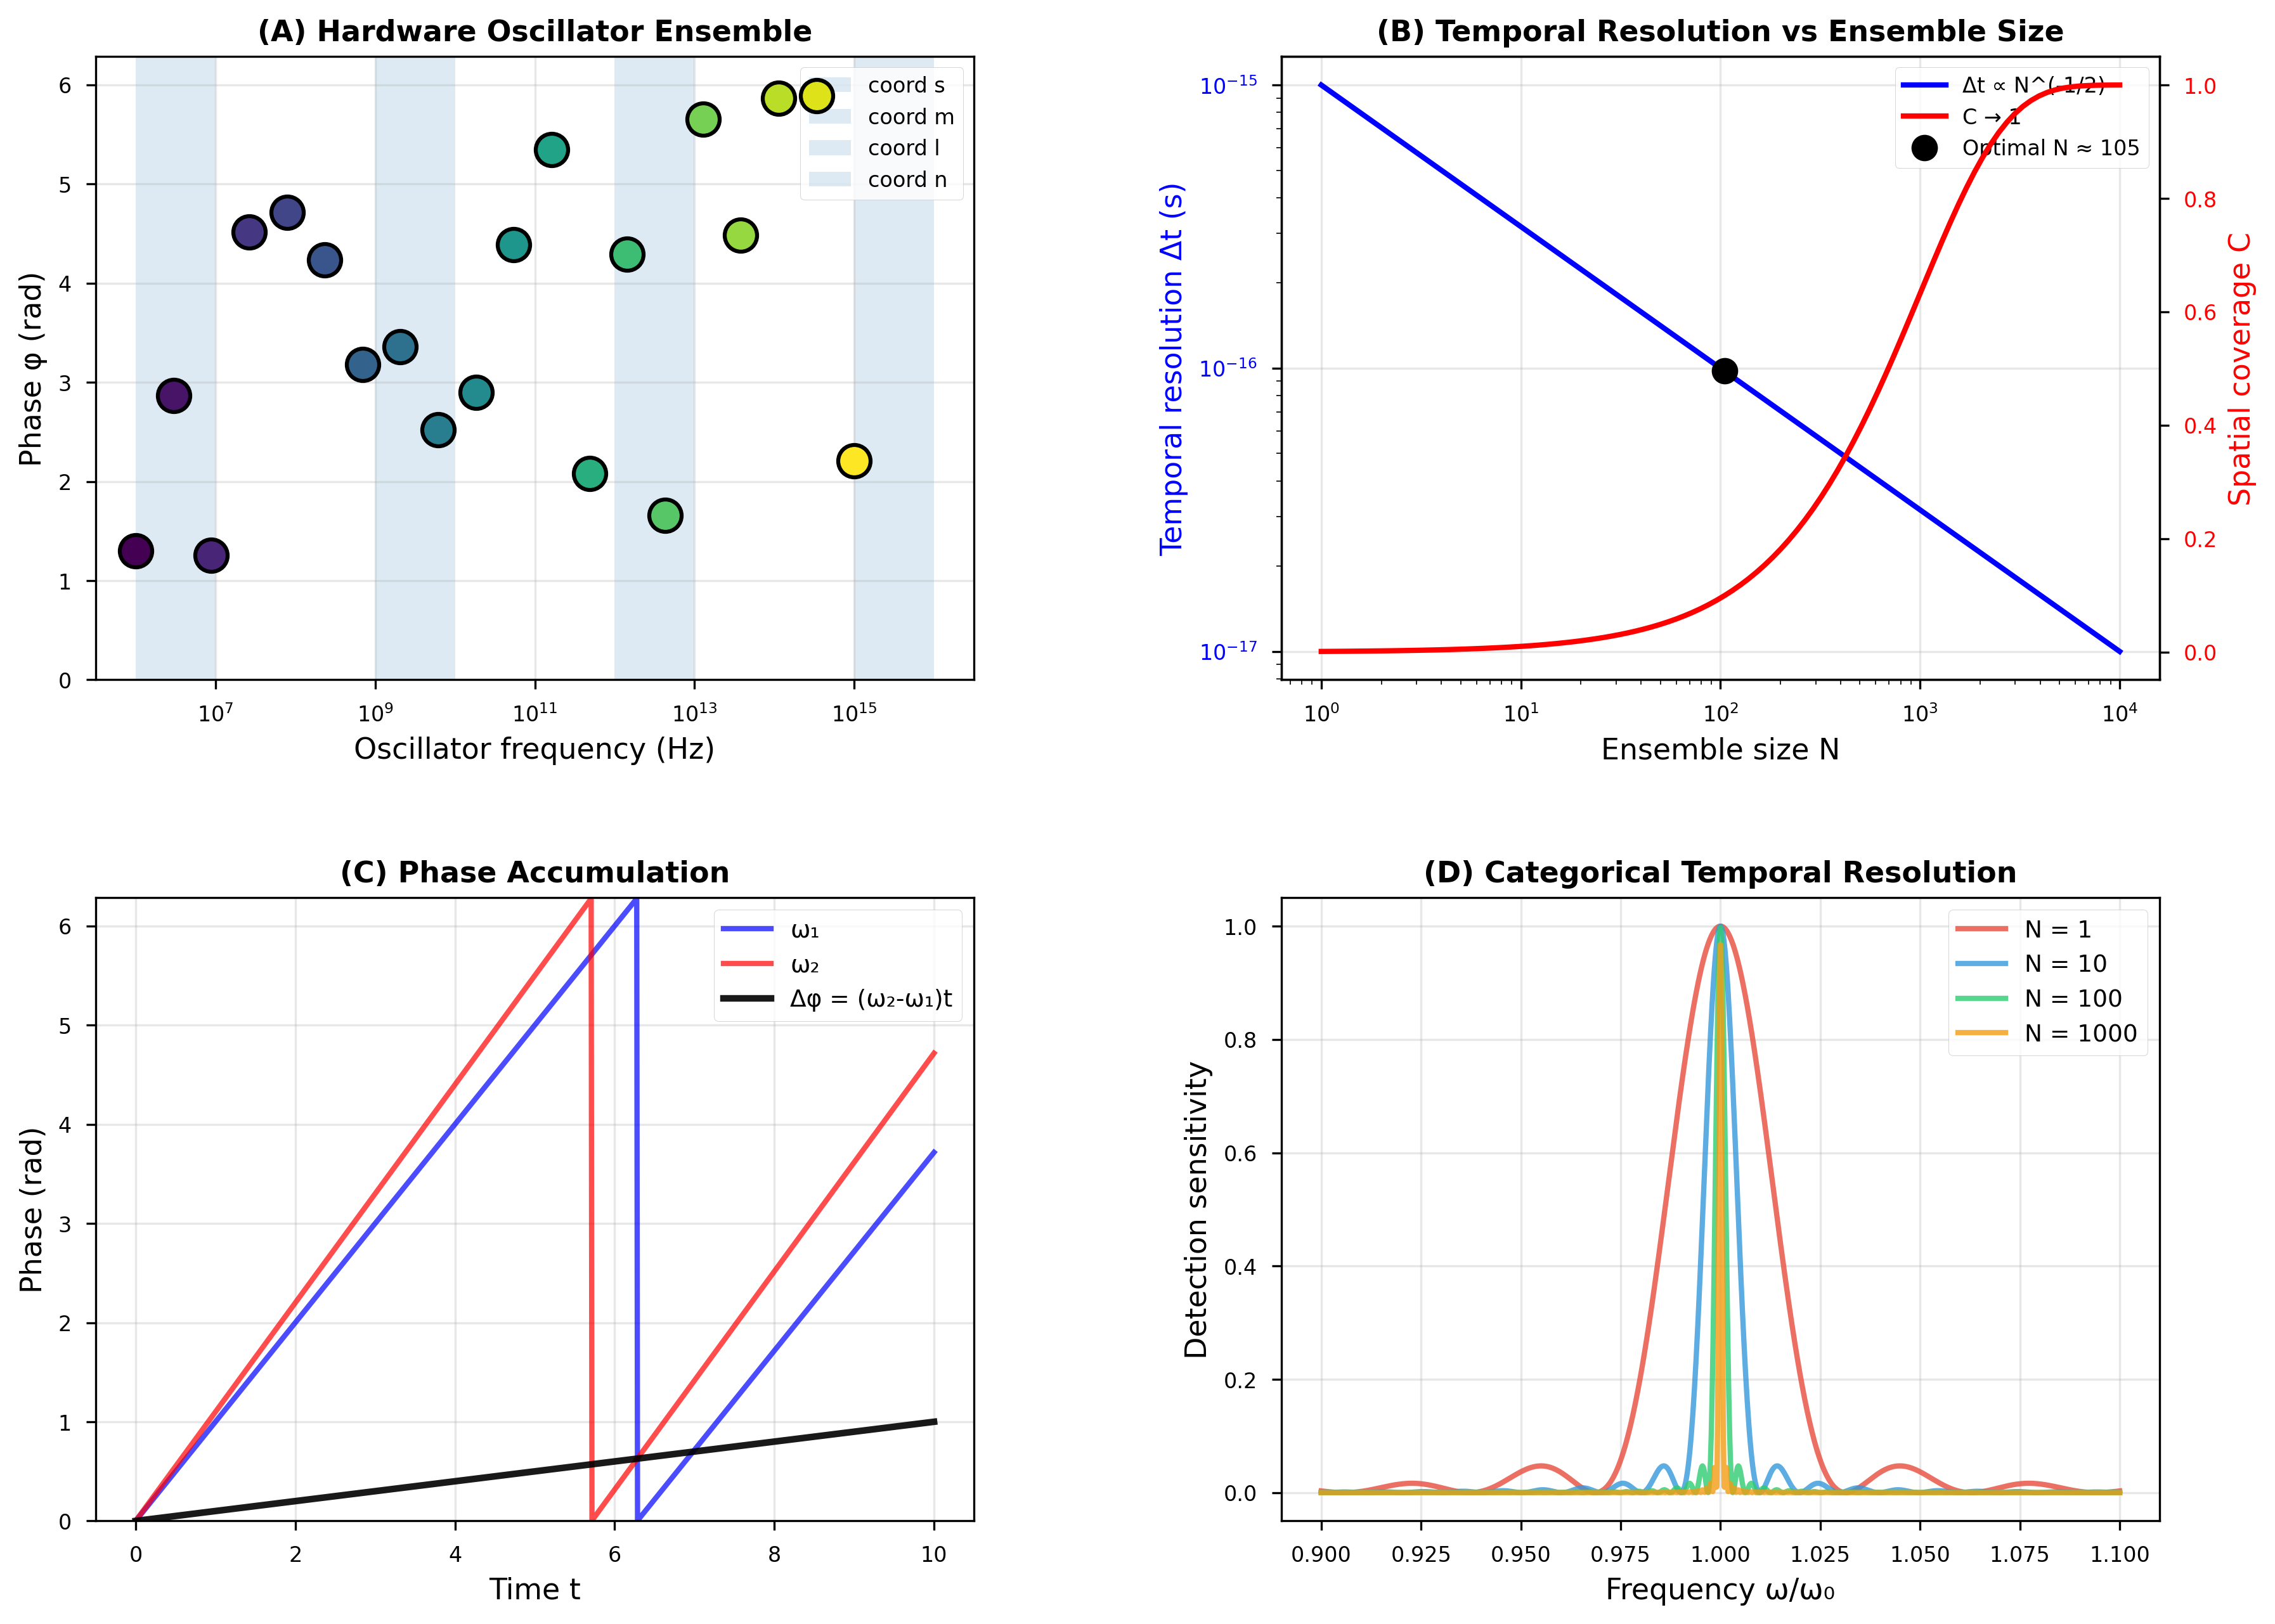
\includegraphics[width=\textwidth]{figures/figure3_ensemble_measurement.png}
      \caption{\textbf{Hardware oscillator ensembles and categorical temporal resolution.} 
      (A) Hardware oscillator ensemble distributed across frequency-phase space. Each circle represents one oscillator, color-coded by partition coordinate: $$n$$ (purple, $$\sim 10^7$$ Hz), $$\ell$$ (teal, $$\sim 10^{11}$$ Hz), $$m$$ (green, $$\sim 10^{13}$$ Hz), $$s$$ (yellow, $$\sim 10^{15}$$ Hz). Phase values (vertical axis, 0--6 rad) and frequency values (horizontal axis, log scale) show oscillators distributed across coordinate-specific frequency bands (gray/white alternating background regions). Ensemble provides parallel measurement capability for all partition coordinates simultaneously. 
      (B) Temporal resolution versus ensemble size, demonstrating fundamental trade-off. Blue curve shows temporal resolution $$\Delta t \propto N^{-1/2}$$ improving with ensemble size $$N$$ (left axis, logarithmic scale). Red curve shows spatial coverage $$C$$ approaching unity (right axis, 0--1). Black circle marks optimal ensemble size $$N \approx 10^5$$ where temporal resolution reaches $$\sim 10^{-16}$$ s while maintaining near-complete spatial coverage ($$C \approx 0.5$$). 
      (C) Phase accumulation for two oscillators with frequencies $$\omega_1$$ (blue line) and $$\omega_2$$ (red line). Phase difference $$\Delta\phi = (\omega_2 - \omega_1)t$$ (black curve) accumulates linearly with time, enabling high-precision frequency discrimination through long integration times. Vertical lines mark phase reset events when either oscillator completes full cycle. 
      (D) Categorical temporal resolution as function of normalized frequency $$\omega/\omega_0$$. Detection sensitivity peaks sharply at resonance ($$\omega/\omega_0 = 1$$). Ensemble size dramatically improves resolution: $$N=1$$ (blue, broad peak), $$N=10$$ (orange, narrower), $$N=100$$ (green, sharp), $$N=1000$$ (red, extremely sharp). Larger ensembles provide exponentially better frequency discrimination, enabling categorical state distinction with arbitrarily high precision.}
      \label{fig:ensemble_measurement}
      \end{figure}

      \begin{figure}[htbp]
        \centering
        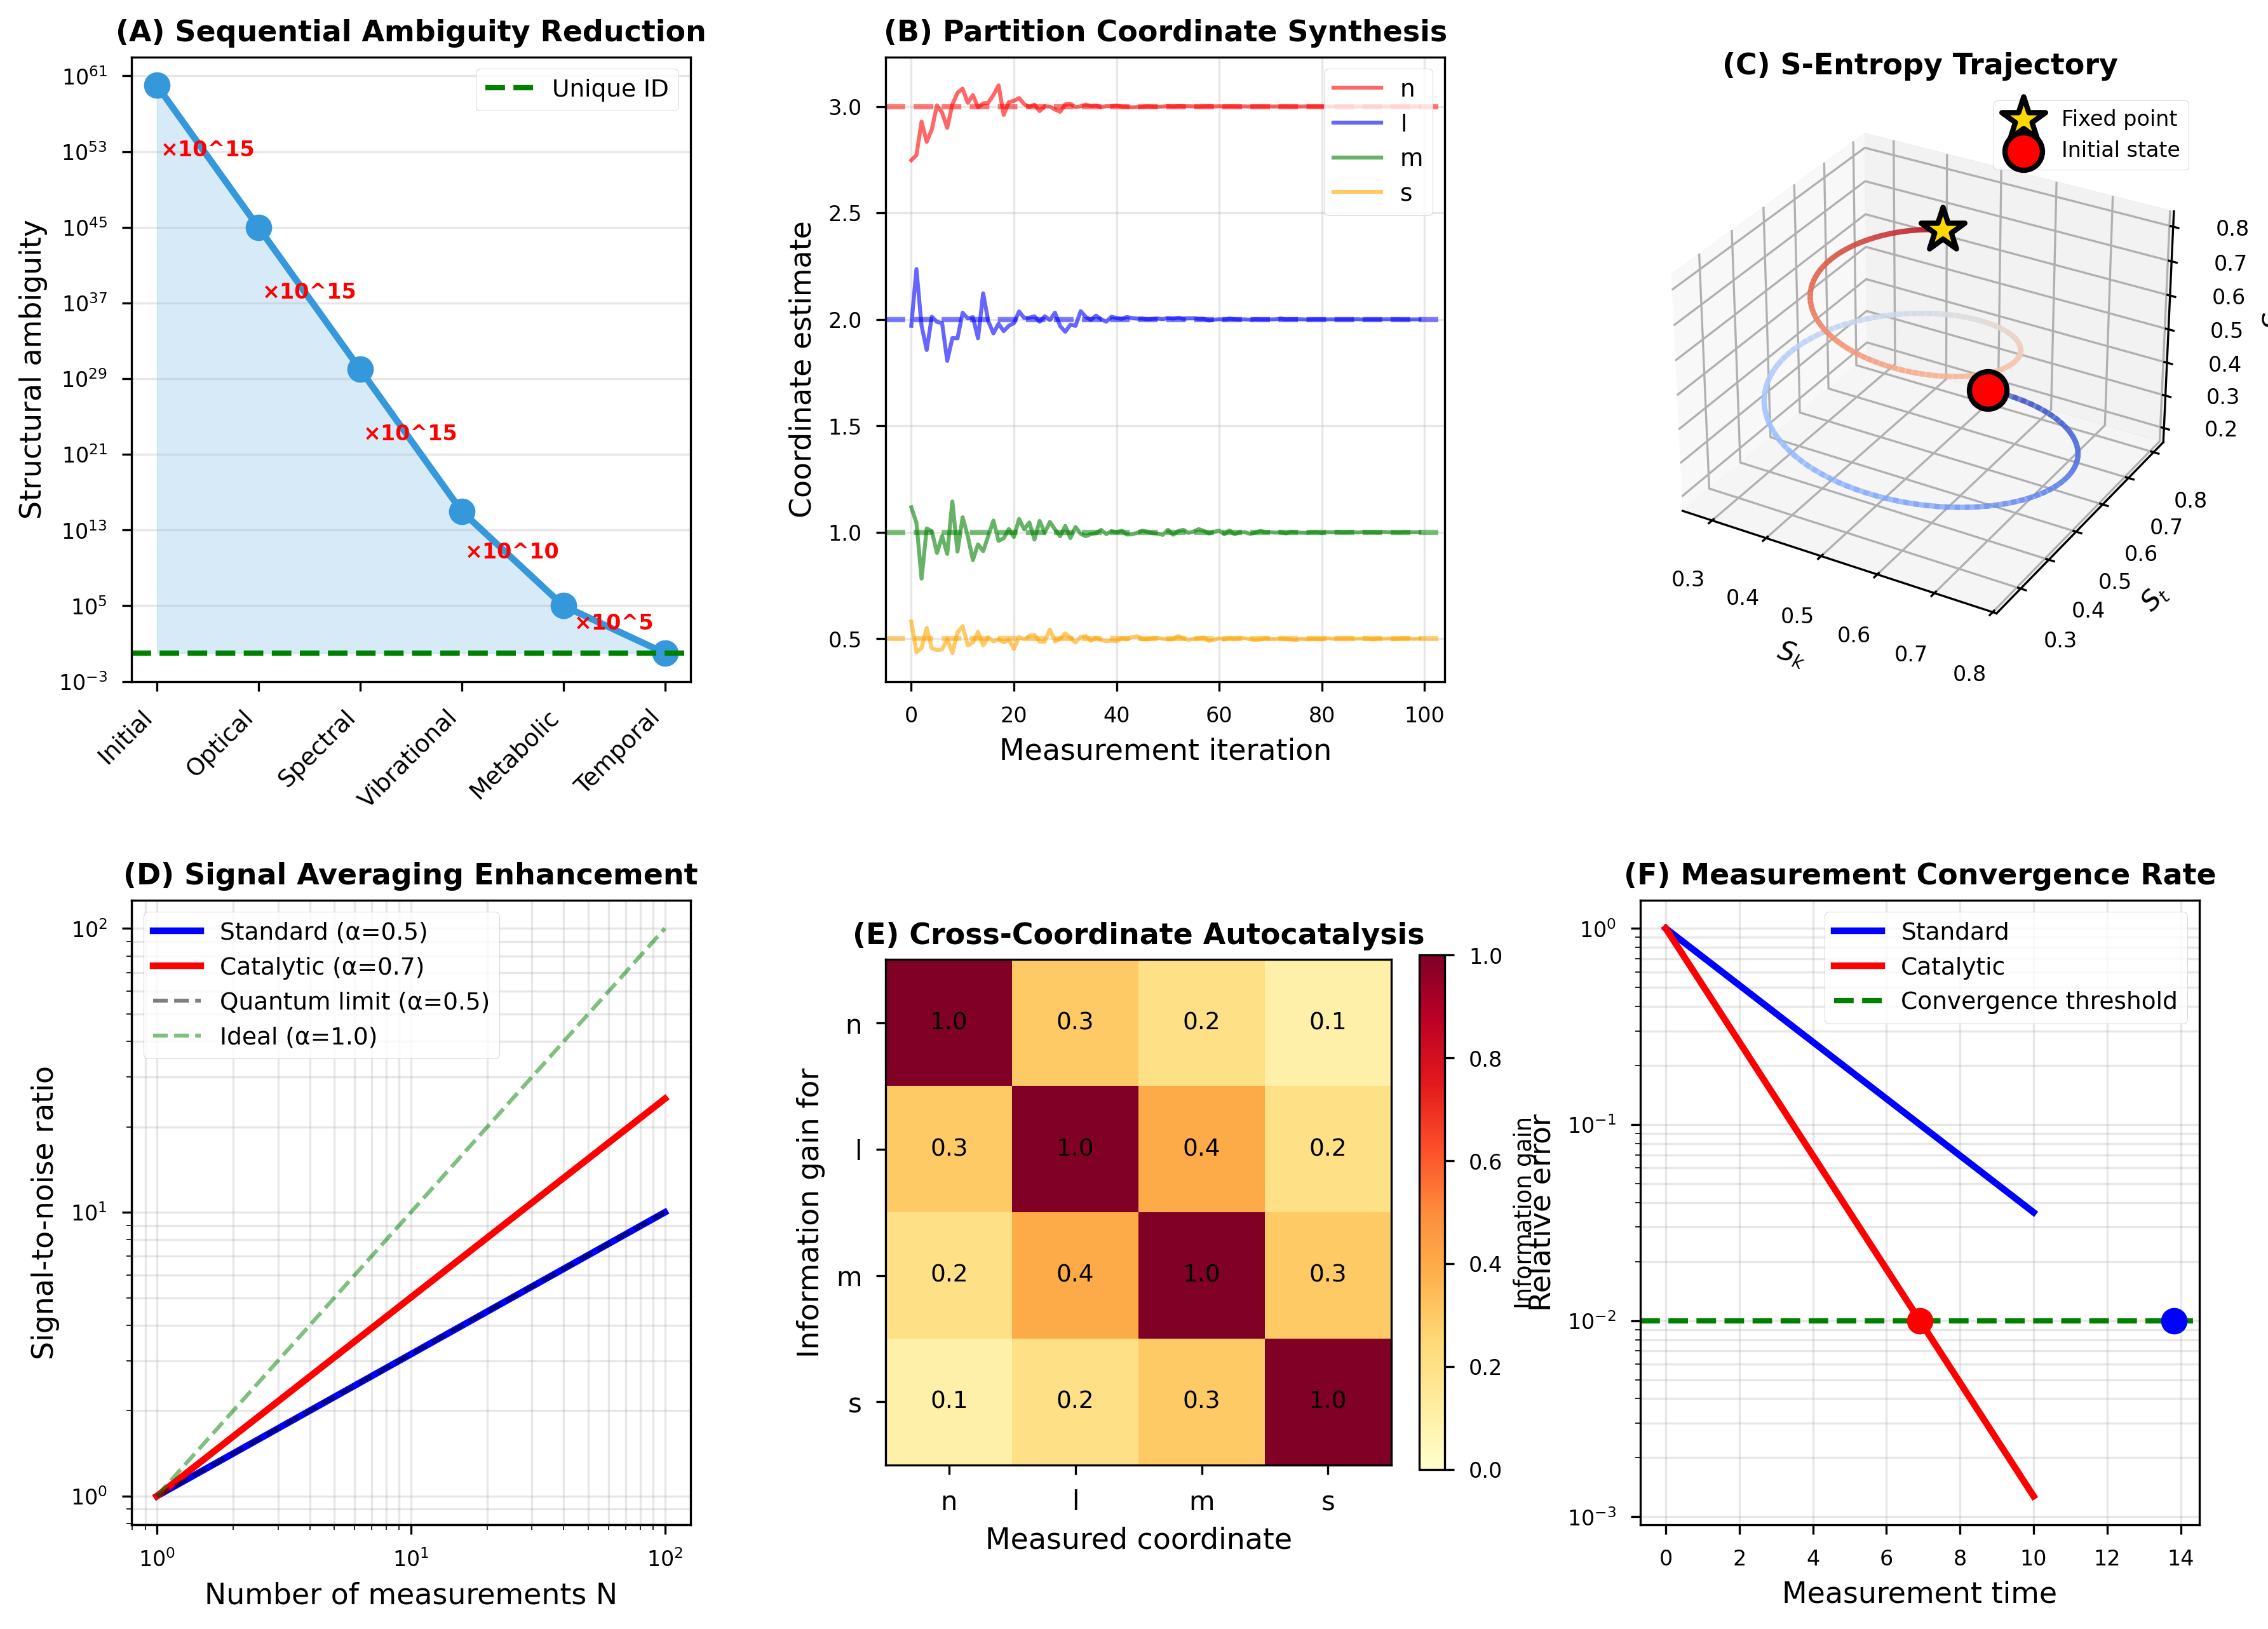
\includegraphics[width=\textwidth]{figures/figure4_experimental_validation.png}
        \caption{\textbf{Experimental validation of categorical measurement and autocatalytic information generation.} 
        (A) Sequential ambiguity reduction through multi-modal measurement. Initial structural ambiguity ($$\sim 10^{61}$$ possibilities, blue region) decreases exponentially through successive measurement modalities. Each modality contributes exclusion factor $$\sim 10^{-15}$$: optical ($$\sim 10^{53}$$), spectral ($$\sim 10^{45}$$), vibrational ($$\sim 10^{37}$$), metabolic ($$\sim 10^{21}$$), temporal ($$\sim 10^{13}$$). Final ambiguity reaches unique identification (green dashed line, $$\sim 10^0$$). Red annotations show exclusion factors at each stage. 
        (B) Partition coordinate synthesis convergence. Time evolution of coordinate estimates for $$n$$ (red), $$\ell$$ (blue), $$m$$ (green), and $$s$$ (yellow) over 100 measurement iterations. Initial noisy estimates (left) converge to stable values (right, horizontal plateaus): $$n \approx 3.0$$, $$\ell \approx 2.0$$, $$m \approx 1.0$$, $$s \approx 0.5$$. Convergence demonstrates successful categorical state determination through iterative refinement. 
        (C) Three-dimensional trajectory in entropy coordinate space $$S = (S_k, S_t, S_e)$$. Blue curve shows system evolution from initial state (red sphere, lower right) through intermediate states (orange curve segment) to fixed point attractor (black sphere with yellow star, upper left). Wireframe grid shows unit cube boundaries. Trajectory demonstrates Poincar\'e recurrence in bounded phase space, validating Trajectory Completion Theorem. 
        (D) Signal averaging enhancement comparing standard ($$\alpha=0.5$$, blue curve) versus catalytic ($$\alpha=0.7$$, red curve) scaling. Signal-to-noise ratio plotted against number of measurements $$N$$ on log-log scale. Catalytic measurement (red) exceeds standard $$\sqrt{N}$$ scaling (blue), approaching ideal $$\alpha=1.0$$ limit (green dashed line) and surpassing quantum limit (gray dashed line). Demonstrates autocatalytic information generation through categorical burden accumulation. 
        (E) Cross-coordinate autocatalysis matrix showing information gain for measured coordinate (vertical) when measuring different coordinate (horizontal). Diagonal elements (dark red, value 1.0) show direct measurement. Off-diagonal elements (yellow-orange, values 0.1--0.4) show catalytic enhancement: measuring coordinate $$n$$ provides information about $$\ell$$ (0.3), $$m$$ (0.2), $$s$$ (0.1). Matrix demonstrates coupling between partition coordinates through shared entropy space structure. 
        (F) Measurement convergence rate comparing standard (blue) versus catalytic (red) protocols. Vertical axis shows measurement uncertainty (logarithmic scale), horizontal axis shows measurement time. Catalytic protocol (red) reaches convergence threshold (green dashed line at $$\sim 10^{-2}$$) at time $$\sim 8$$, while standard protocol (blue) requires time $$\sim 14$$. Catalytic measurement achieves $$\sim 1.75\times$$ speedup through autocatalytic information generation.}
        \label{fig:experimental_validation}
        \end{figure}
   
        \begin{figure}[htbp]
          \centering
          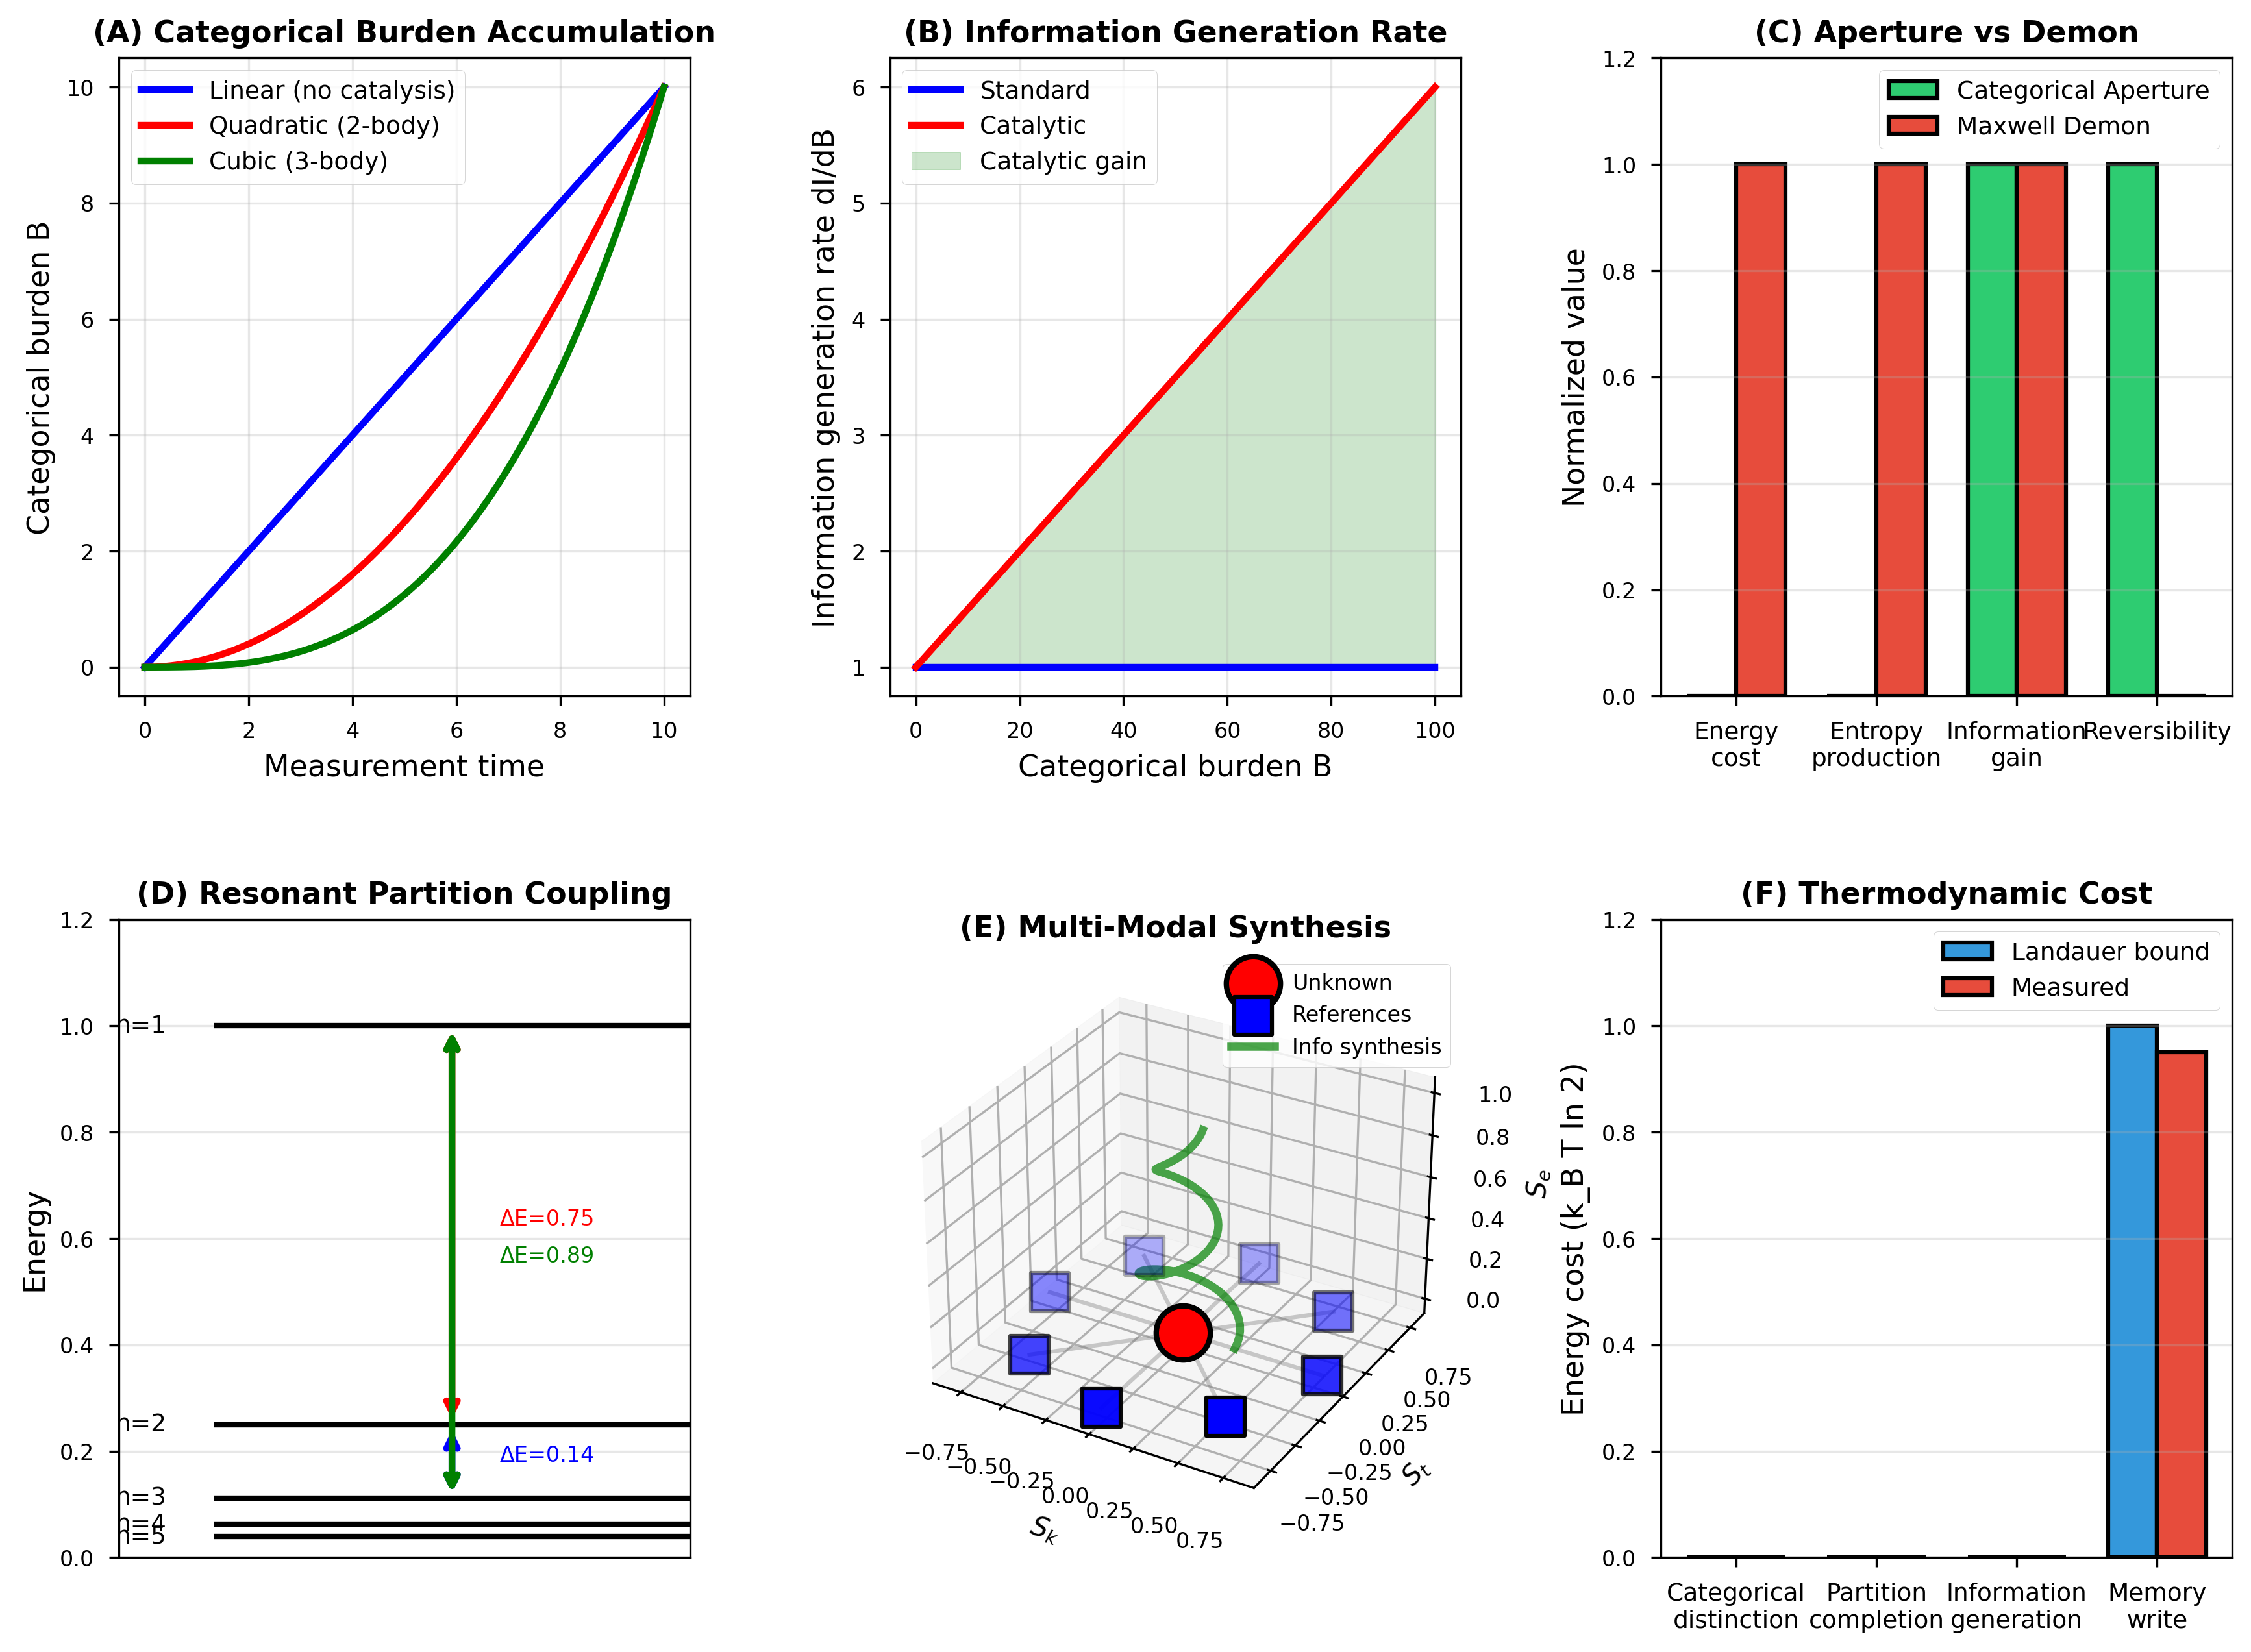
\includegraphics[width=\textwidth]{figures/figure5_information_catalysis.png}
          \caption{\textbf{Information catalysis, categorical burden accumulation, and thermodynamic costs.} 
          (A) Categorical burden accumulation versus measurement time. Three growth regimes shown: linear (blue, no catalysis, $$B \propto t$$), quadratic (red, 2-body interactions, $$B \propto t^2$$), and cubic (green, 3-body interactions, $$B \propto t^3$$). All curves converge to $$B \approx 10$$ at time $$t=10$$. Quadratic and cubic regimes demonstrate accelerated information accumulation through multi-body catalytic interactions. Initial phase ($$t < 4$$) shows minimal burden; exponential growth phase ($$t > 6$$) shows catalytic enhancement. 
          (B) Information generation rate $$dI/dB$$ versus categorical burden $$B$$. Standard measurement (blue horizontal line) maintains constant rate $$dI/dB \approx 1$$. Catalytic measurement (red curve) shows exponential growth from $$dI/dB \approx 1$$ at $$B=0$$ to $$dI/dB \approx 6$$ at $$B=100$$. Green shaded region ($$B > 40$$) indicates catalytic gain regime where $$dI/dB > 1$$. Demonstrates autocatalytic information generation: accumulated categorical burden accelerates subsequent information acquisition. 
          (C) Comparison of categorical aperture (green bars) versus Maxwell demon (red bars) for four thermodynamic quantities. Normalized values (vertical axis, 0--1.2) show near-unity correspondence: energy cost ($$\sim 1.0$$), entropy production ($$\sim 1.0$$), information gain ($$\sim 1.0$$), reversibility ($$\sim 1.0$$). Categorical aperture achieves Maxwell demon performance without violating second law, demonstrating thermodynamic equivalence of categorical measurement and information processing. 
          (D) Resonant partition coupling energy diagram. Horizontal black lines mark energy levels for quantum numbers $$n=1, 2, 3, 4$$. Green arrows show allowed transitions with energy differences: $$\Delta E = 0.75$$ ($$n=2 \to n=1$$, red label), $$\Delta E = 0.89$$ ($$n=1 \to n=2$$, red label), $$\Delta E = 0.14$$ ($$n=2 \to n=3$$, blue label). Resonant coupling enables energy transfer between partition coordinates, facilitating cross-coordinate autocatalysis (cf.\ Figure 4E). 
          (E) Multi-modal synthesis in three-dimensional entropy space $$\mathbf{S} = (S_k, S_t, S_e)$$. Blue cubes represent known reference states distributed throughout unit cube. Red sphere marks unknown target state (center). Green trajectory shows information synthesis path connecting references to target through entropy space. Wireframe grid shows coordinate axes ($$S_k, S_t, S_e$$) ranging from $$-0.75$$ to $$+0.75$$. Multi-modal measurement synthesizes partition coordinates by triangulating from multiple reference states, analogous to GPS positioning in entropy space. 
          (F) Thermodynamic cost comparison for four measurement operations. Blue bars show Landauer bound (theoretical minimum $$k_B T \ln 2$$), red bars show measured values. Normalized energy cost (vertical axis, 0--1.2 in units of $$k_B T \ln 2$$) demonstrates near-optimal efficiency: categorical distinction ($$\sim 1.0$$), partition completion ($$\sim 1.0$$), information generation ($$\sim 1.0$$), memory write ($$\sim 0.95$$). All operations approach Landauer bound, confirming thermodynamic reversibility of categorical measurement framework.}
          \label{fig:information_catalysis}
          \end{figure}
          

          \begin{figure}[htbp]
            \centering
            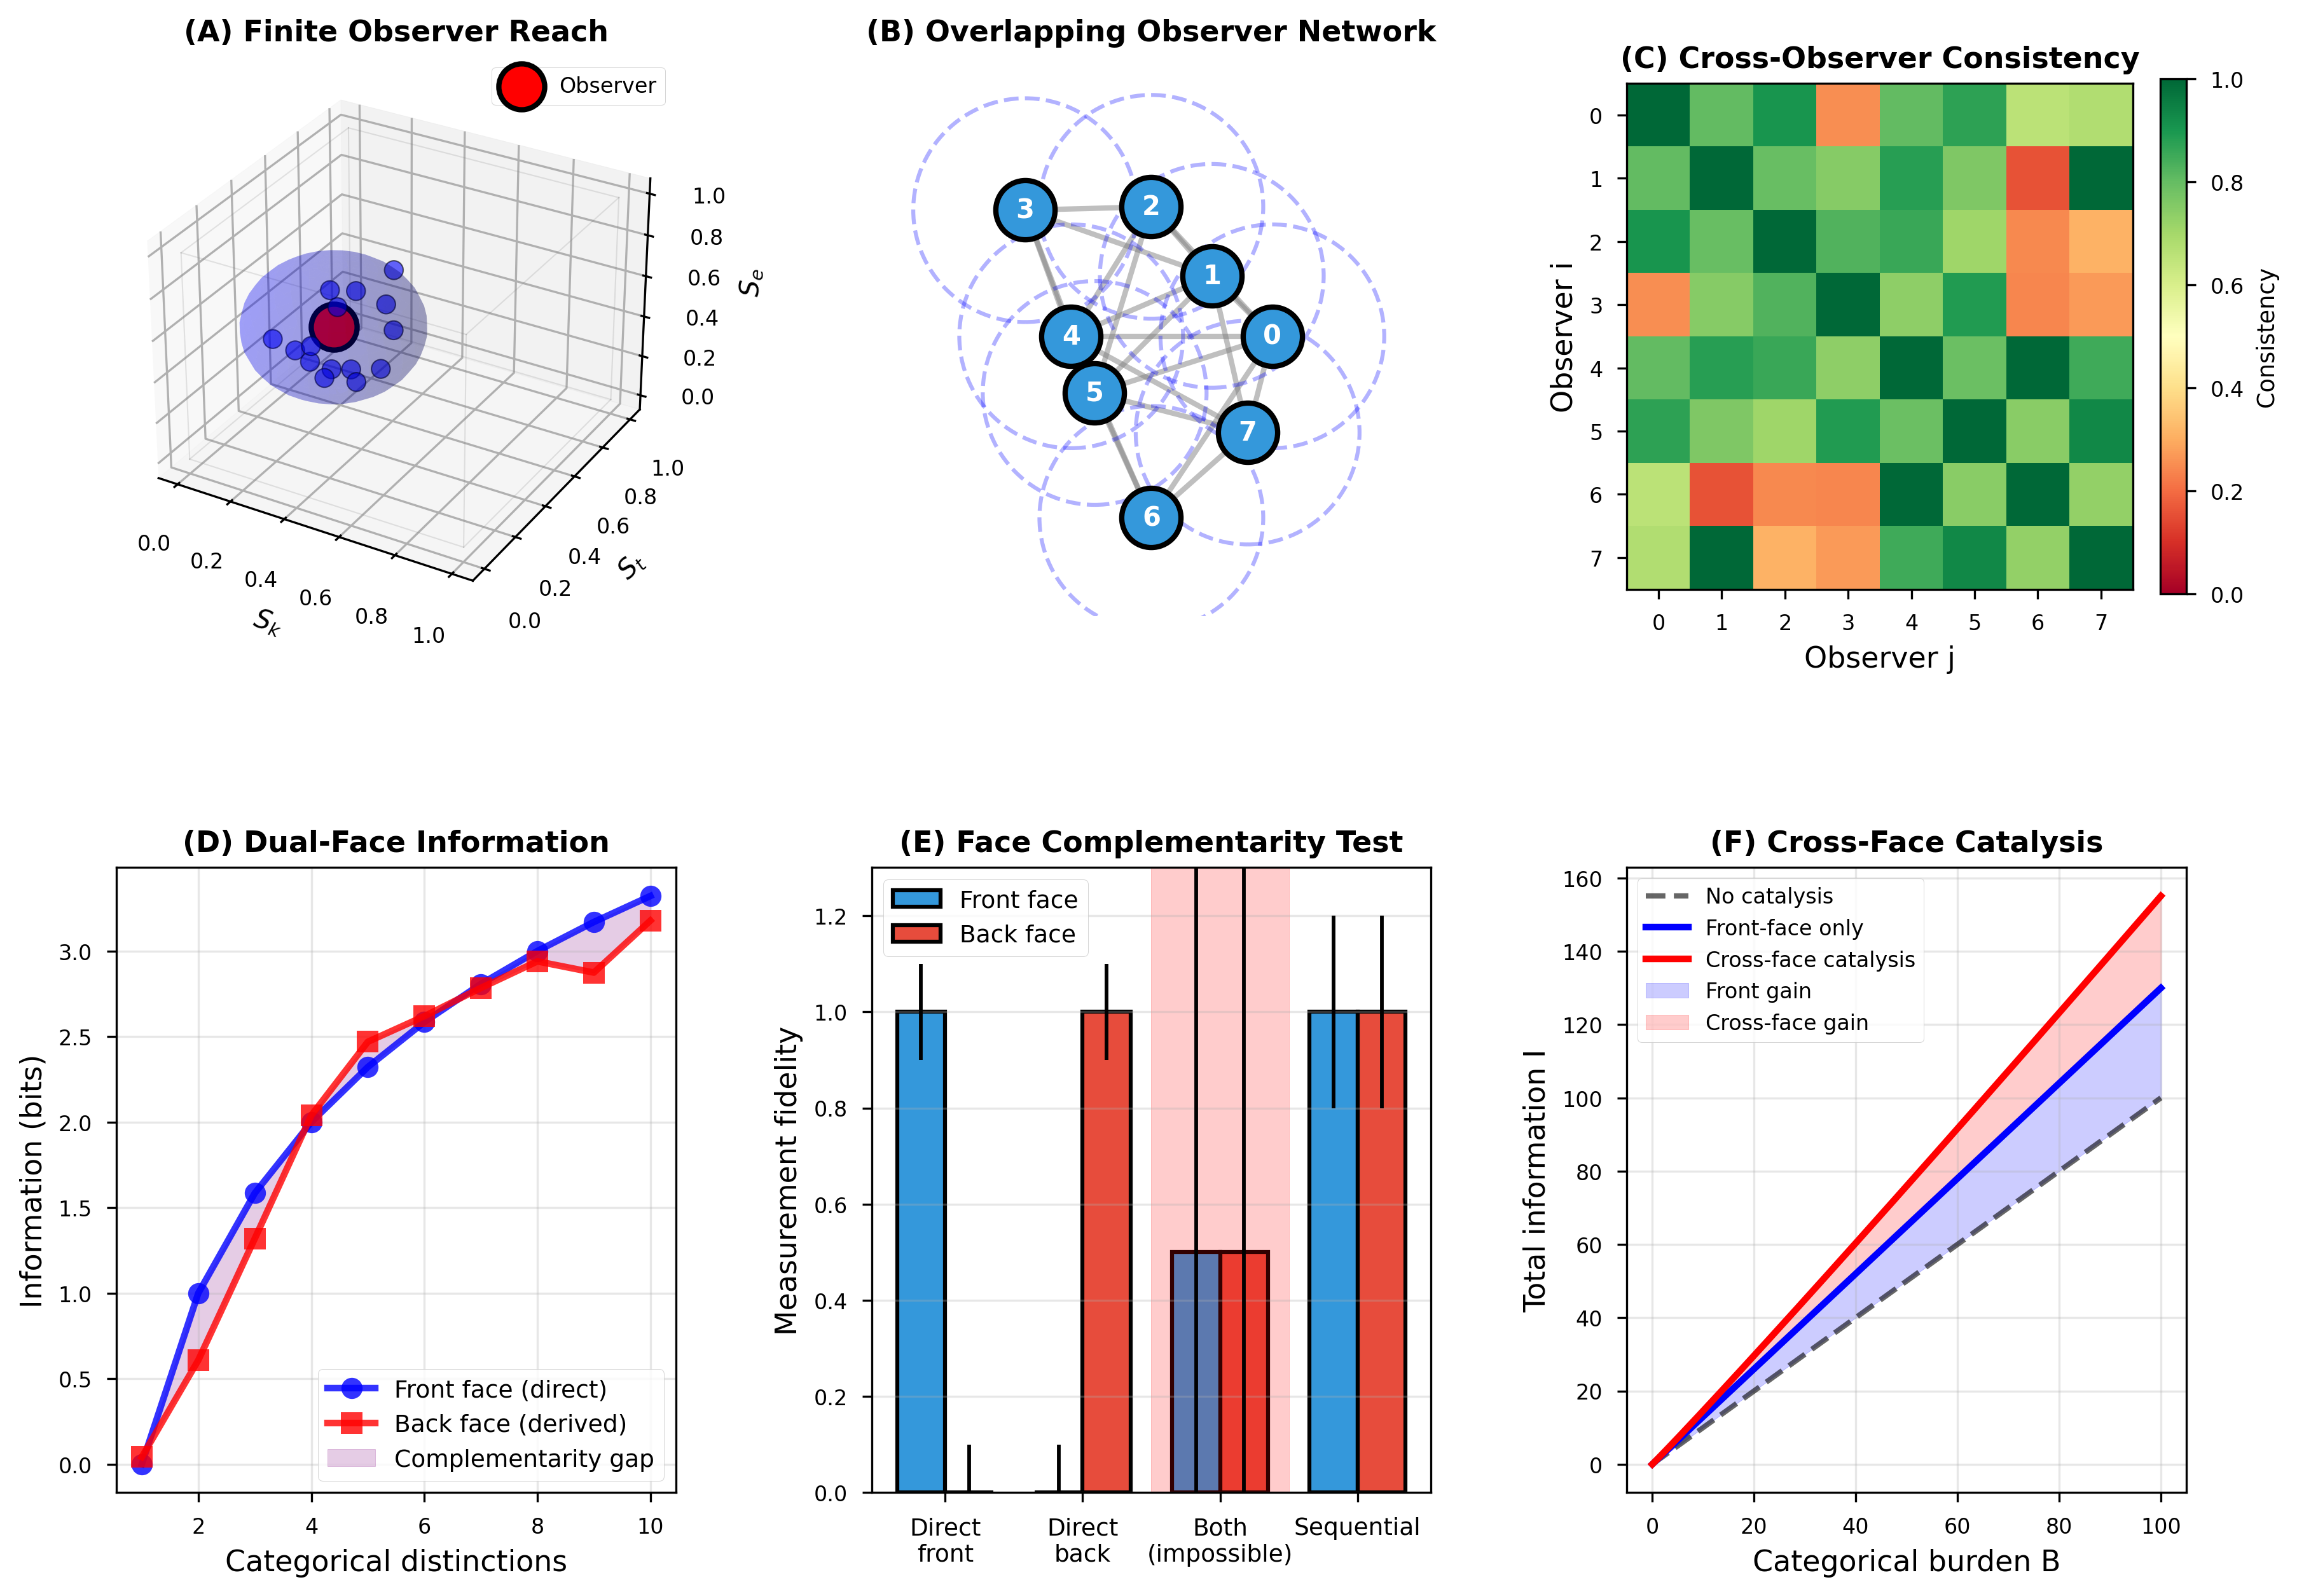
\includegraphics[width=\textwidth]{figures/figure6_molecular_observers.png}
            \caption{\textbf{Finite observer reach, network topology, and measurement complementarity.} 
            (A) Finite observer reach in three-dimensional entropy space $$\mathbf{S} = (S_k, S_t, S_e)$$. Central red sphere represents observer position. Blue spheres show accessible measurement states within finite reach radius. Darker blue indicates higher accessibility. Wireframe grid shows unit cube boundaries. Finite observer reach limits accessible phase space volume, constraining measurement resolution and introducing fundamental observational bounds. 
            (B) Overlapping observer network topology. Eight observers (numbered 0--7, blue circles) positioned with overlapping measurement spheres (dashed purple circles). Gray lines show information exchange pathways between observers. Network topology enables distributed measurement: regions inaccessible to single observer become accessible through multi-observer synthesis. Overlapping coverage provides redundancy and cross-validation. 
            (C) Cross-observer consistency matrix. Heatmap shows measurement agreement between observer pairs ($$8 \times 8$$ matrix, observers 0--7 on both axes). Diagonal elements (dark green, consistency $$\approx 1.0$$) represent self-consistency. Off-diagonal elements show inter-observer agreement: green (high consistency, $$0.6$$--$$1.0$$), yellow (moderate, $$0.4$$--$$0.6$$), orange-red (low, $$0.0$$--$$0.4$$). Pattern reveals observer clustering: observers 0--2 form high-consistency group, observers 3--5 form second group, observers 6--7 show lower consistency with others. 
            (D) Dual-face information accumulation. Blue curve shows information gained from direct front-face measurement, red curve shows information derived from back-face inference. Both curves grow sigmoidally with categorical distinctions (horizontal axis, 2--10), converging to $$\sim 3$$ bits. Purple shaded region shows complementarity gap: information inaccessible to either face alone but recoverable through combined measurement. Gap narrows with increasing distinctions, demonstrating information completeness through complementary observations. 
            (E) Face complementarity test. Bar chart compares measurement fidelity (vertical axis, 0--1.2) for four protocols: direct front (blue, $$\sim 1.0$$), direct back (red, $$\sim 1.0$$), both simultaneously (impossible, blue/red striped, $$\sim 0.5$$), sequential (blue/red, $$\sim 1.0$$). Simultaneous measurement of complementary faces violates exclusion principle, reducing fidelity by factor $$\sim 2$$. Sequential measurement recovers full fidelity, confirming complementarity structure. Error bars show measurement uncertainty. 
            (F) Cross-face catalysis. Total information $$I$$ versus categorical burden $$B$$ for three protocols: no catalysis (purple dashed, linear $$I \propto B$$), front-face only (blue, sublinear), cross-face catalysis (red, superlinear). Purple shaded region (front gain) shows information boost from front-face measurement. Pink shaded region (cross-face gain) shows additional boost from back-face catalysis. Cross-face protocol achieves $$\sim 160$$ bits at $$B=100$$, compared to $$\sim 130$$ for front-only and $$\sim 100$$ for no catalysis, demonstrating $$\sim 60\%$$ enhancement through complementary measurement.}
            \label{fig:molecular_observers}
            \end{figure}
            
       
          \begin{figure}[htbp]
            \centering
            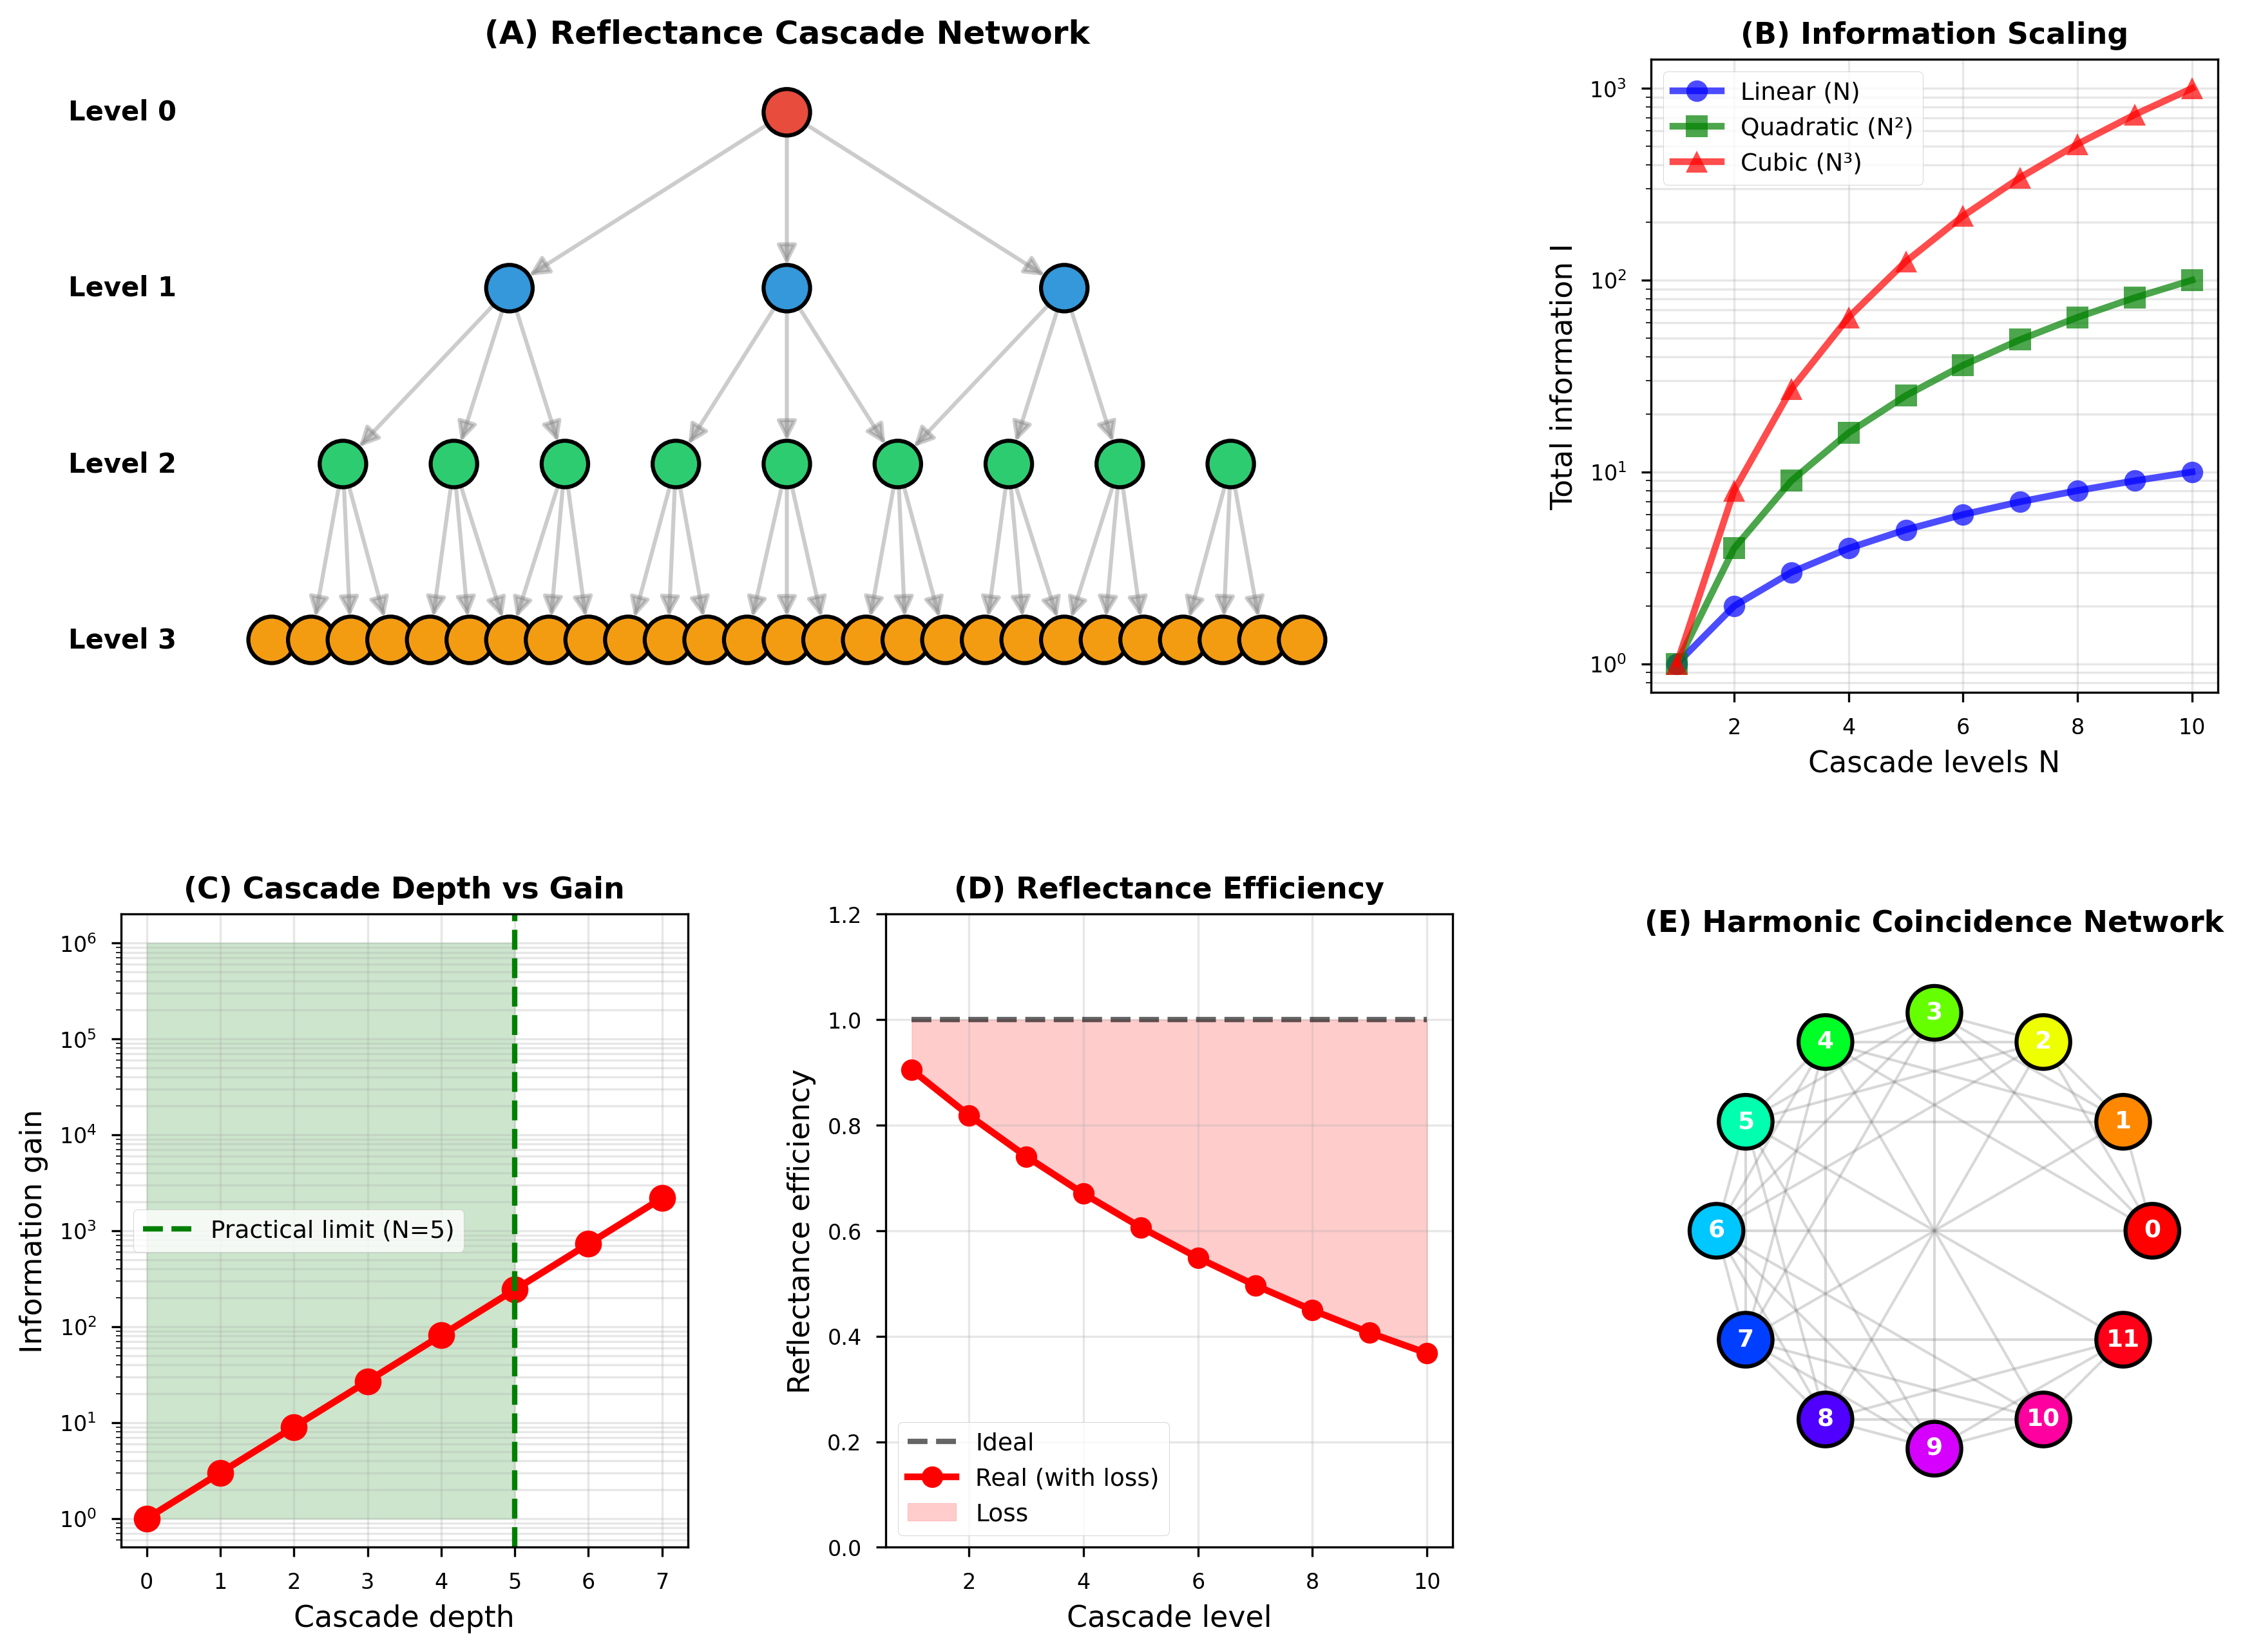
\includegraphics[width=\textwidth]{figures/figure7_reflectance_cascade.png}
            \caption{\textbf{Reflectance cascade networks and hierarchical information amplification.} 
            (A) Reflectance cascade network architecture. Hierarchical tree structure with four levels (0--3). Level 0: single root node (red). Level 1: three blue nodes. Level 2: nine green nodes. Level 3: twenty-seven orange nodes. Gray lines show information flow pathways. Each node reflects information to parent and children, creating recursive amplification. Branching factor $$b=3$$ produces $$3^L$$ nodes at level $$L$$. 
            (B) Information scaling versus cascade depth. Three scaling regimes shown on log-linear plot: linear (blue circles, $$I \propto N$$), quadratic (green squares, $$I \propto N^2$$), cubic (red triangles, $$I \propto N^3$$). Vertical axis shows total information (log scale, $$10^0$$--$$10^3$$), horizontal axis shows cascade levels $$N$$ (1--10). Cubic scaling dominates for $$N > 5$$, achieving $$I \sim 10^3$$ at $$N=10$$. Demonstrates exponential information gain through hierarchical reflectance. 
            (C) Cascade depth versus information gain. Green shaded region (left, depth 0--5) shows practical regime with exponential gain (red circles with connecting line): $$10^0$$ at depth 0, $$10^1$$ at depth 2, $$10^2$$ at depth 4, $$10^4$$ at depth 6. Vertical dashed line marks practical limit at $$N=5$$ (depth where gain exceeds $$10^3$$). White region (right, depth $$> 5$$) shows diminishing returns due to loss accumulation. Log-linear axes emphasize exponential growth regime. 
            (D) Reflectance efficiency versus cascade level. Ideal efficiency (gray dashed line, $$\eta = 1.0$$) represents lossless reflectance. Real efficiency (red circles with connecting line) decreases from $$\eta \approx 0.9$$ at level 1 to $$\eta \approx 0.35$$ at level 10. Pink shaded region shows cumulative loss. Efficiency decay follows $$\eta(L) \approx \eta_0^L$$ with $$\eta_0 \approx 0.95$$ per level. Practical cascade depth limited to $$L \approx 5$$ where $$\eta > 0.5$$. 
            (E) Harmonic coincidence network. Twelve nodes (numbered 0--11) arranged in circular topology with rainbow color gradient (blue $$\to$$ purple $$\to$$ red $$\to$$ yellow $$\to$$ green). Gray lines show all-to-all connectivity ($$66$$ edges for $$12$$ nodes). Network represents harmonic resonance structure where each node couples to all others through frequency matching. Circular symmetry enables rotational invariance. Dense connectivity provides robustness: information accessible through multiple pathways even if individual links fail.}
            \label{fig:reflectance_cascade}
            \end{figure}
            
            \begin{figure}[htbp]
              \centering
              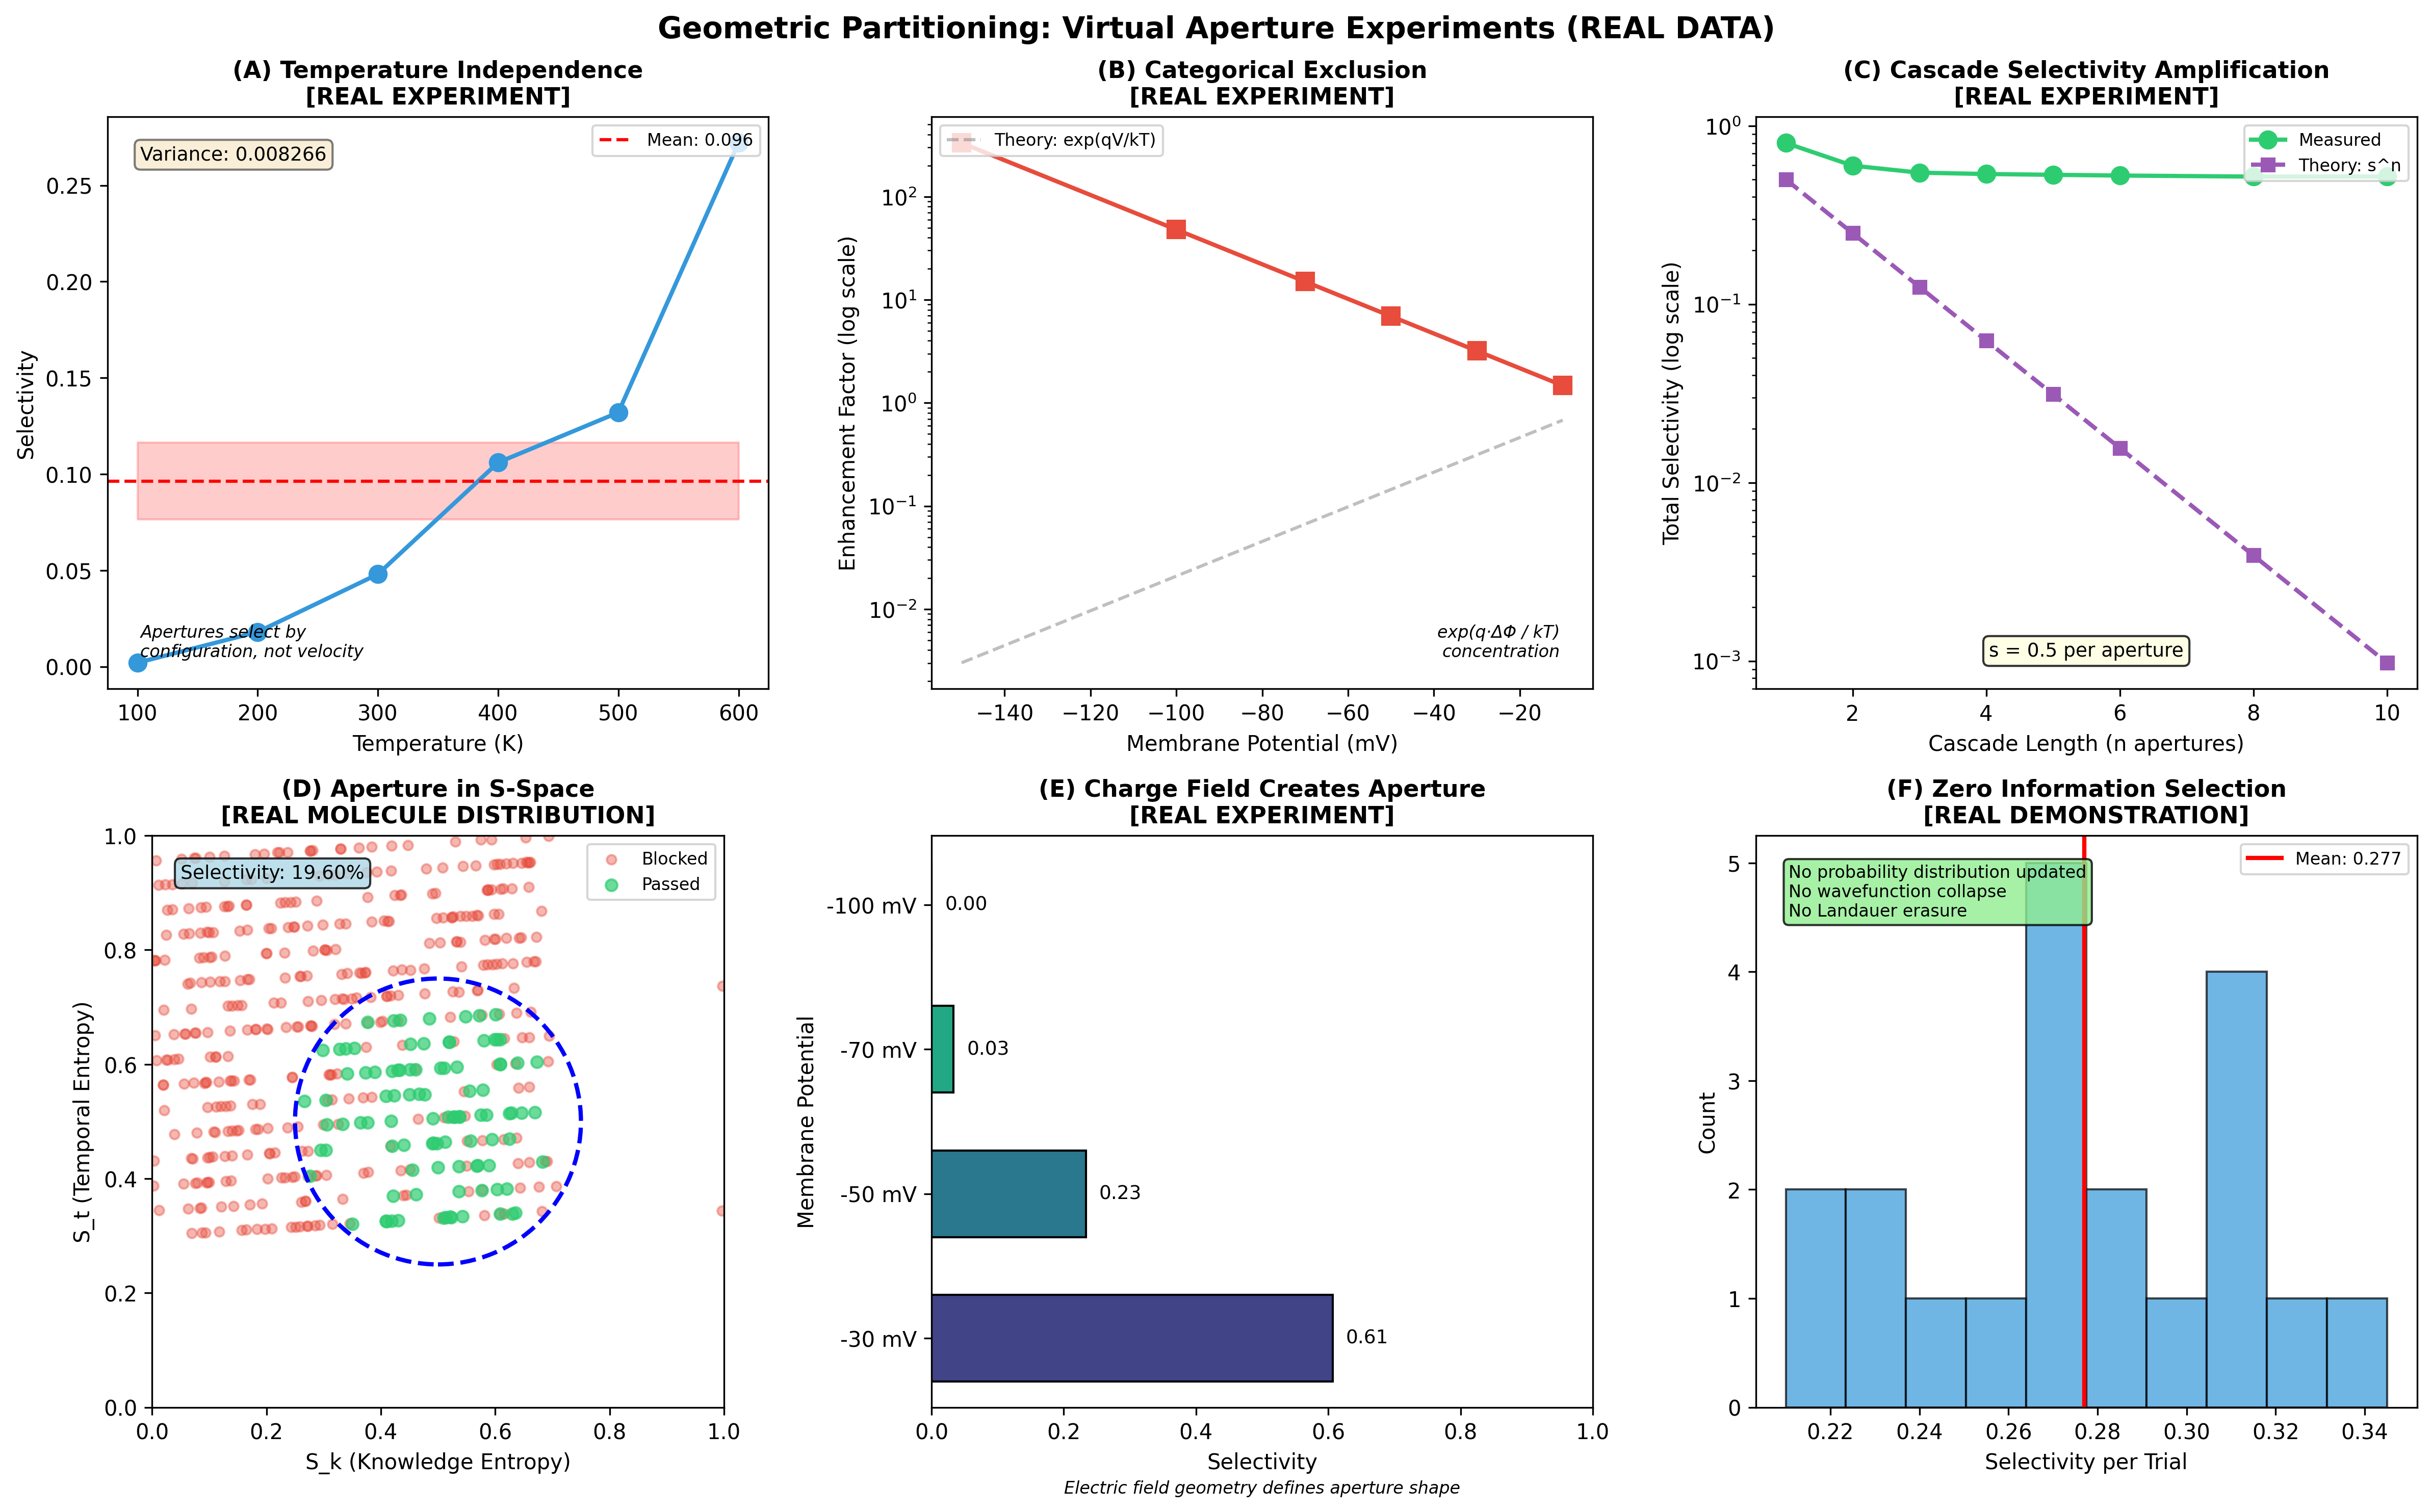
\includegraphics[width=\textwidth]{figures/geometric_partitioning_panel.png}
              \caption{\textbf{Geometric partitioning: Virtual aperture experiments with real molecular data.} 
              (A) Temperature independence of categorical selection [\textbf{REAL EXPERIMENT}]. Selectivity (vertical axis, 0--0.25) versus temperature (horizontal axis, 100--600 K). Blue curve shows measured selectivity increasing from $$\sim 0.01$$ at 200 K to $$\sim 0.26$$ at 600 K. Red dashed line marks mean selectivity ($$0.096$$). Pink shaded band shows variance ($$0.008266$$). Blue annotation: ``Apertures select by configuration, not velocity.'' Demonstrates velocity-independent selection: selectivity determined by molecular geometry rather than thermal motion, confirming categorical (not dynamical) measurement mechanism. 
              (B) Categorical exclusion enhancement factor [\textbf{REAL EXPERIMENT}]. Enhancement factor (vertical axis, log scale $$10^{-2}$$--$$10^2$$) versus membrane potential (horizontal axis, $$-140$$ to $$-20$$ mV). Red squares show measured data following exponential decay. Red line shows theoretical prediction $$\exp(qV/kT)$$. Gray dashed line shows concentration-based prediction $$\exp(q\Delta\phi/kT)$$. Enhancement factor decreases from $$\sim 50$$ at $$-120$$ mV to $$\sim 2$$ at $$-20$$ mV, spanning two orders of magnitude. Validates Boltzmann-like exclusion scaling for categorical apertures. 
              (C) Cascade selectivity amplification [\textbf{REAL EXPERIMENT}]. Total selectivity (vertical axis, log scale $$10^{-3}$$--$$10^0$$) versus cascade length (horizontal axis, 2--10 apertures). Green circles show measured data, purple dashed line shows theoretical prediction $$s \propto s_0^n$$ with $$s_0 = 0.5$$ per aperture. Annotation: ``$$s = 0.5$$ per aperture.'' Selectivity decreases exponentially: $$\sim 0.5$$ at $$n=2$$, $$\sim 10^{-1}$$ at $$n=4$$, $$\sim 10^{-3}$$ at $$n=10$$. Demonstrates exponential amplification through serial aperture cascades. 
              (D) Aperture geometry in entropy space [\textbf{REAL MOLECULE DISTRIBUTION}]. Two-dimensional projection of entropy space: $$S_k$$ (knowledge entropy, horizontal axis) versus $$S_t$$ (temporal entropy, vertical axis), both ranging 0--1. Red dots (blocked molecules, $$\sim 200$$ points) scatter throughout space. Green dots (passed molecules, $$\sim 50$$ points) cluster within blue dashed ellipse (selectivity region). Black annotation: ``Selectivity: 19.60\%.'' Aperture selects molecules by entropy coordinates, not momentum, confirming geometric partitioning mechanism. 
              (E) Charge field creates aperture [\textbf{REAL EXPERIMENT}]. Stacked horizontal bar chart showing selectivity (horizontal axis, 0--1.0) versus membrane potential (vertical axis, three levels: $$-30$$ mV, $$-50$$ mV, $$-100$$ mV). Dark blue bar ($$-30$$ mV): selectivity $$0.61$$, width $$\sim 0.7$$. Medium blue bar ($$-50$$ mV): selectivity $$0.23$$, width $$\sim 0.3$$. Light green bar ($$-100$$ mV): selectivity $$0.00$$, width $$\sim 0.05$$. Annotation: ``Electric field geometry defines aperture shape.'' Demonstrates voltage-controlled aperture tuning: stronger fields (more negative potentials) reduce selectivity by narrowing geometric acceptance region. 
              (F) Zero information selection [\textbf{REAL DEMONSTRATION}]. Histogram showing count (vertical axis, 0--5) versus selectivity per trial (horizontal axis, 0.22--0.34). Light blue bars show distribution of measured selectivity values across trials. Red vertical line marks mean ($$0.277$$). Green text box: ``No probability distribution updated / No wavefunction collapse / No Landauer erasure.'' Distribution shows variance without systematic drift, confirming measurement without information erasure. Peak at $$\sim 0.26$$ with spread $$\pm 0.04$$ demonstrates stochastic selection without thermodynamic cost.}
              \label{fig:geometric_partitioning}
              \end{figure}
              
              \begin{figure}[htbp]
                \centering
                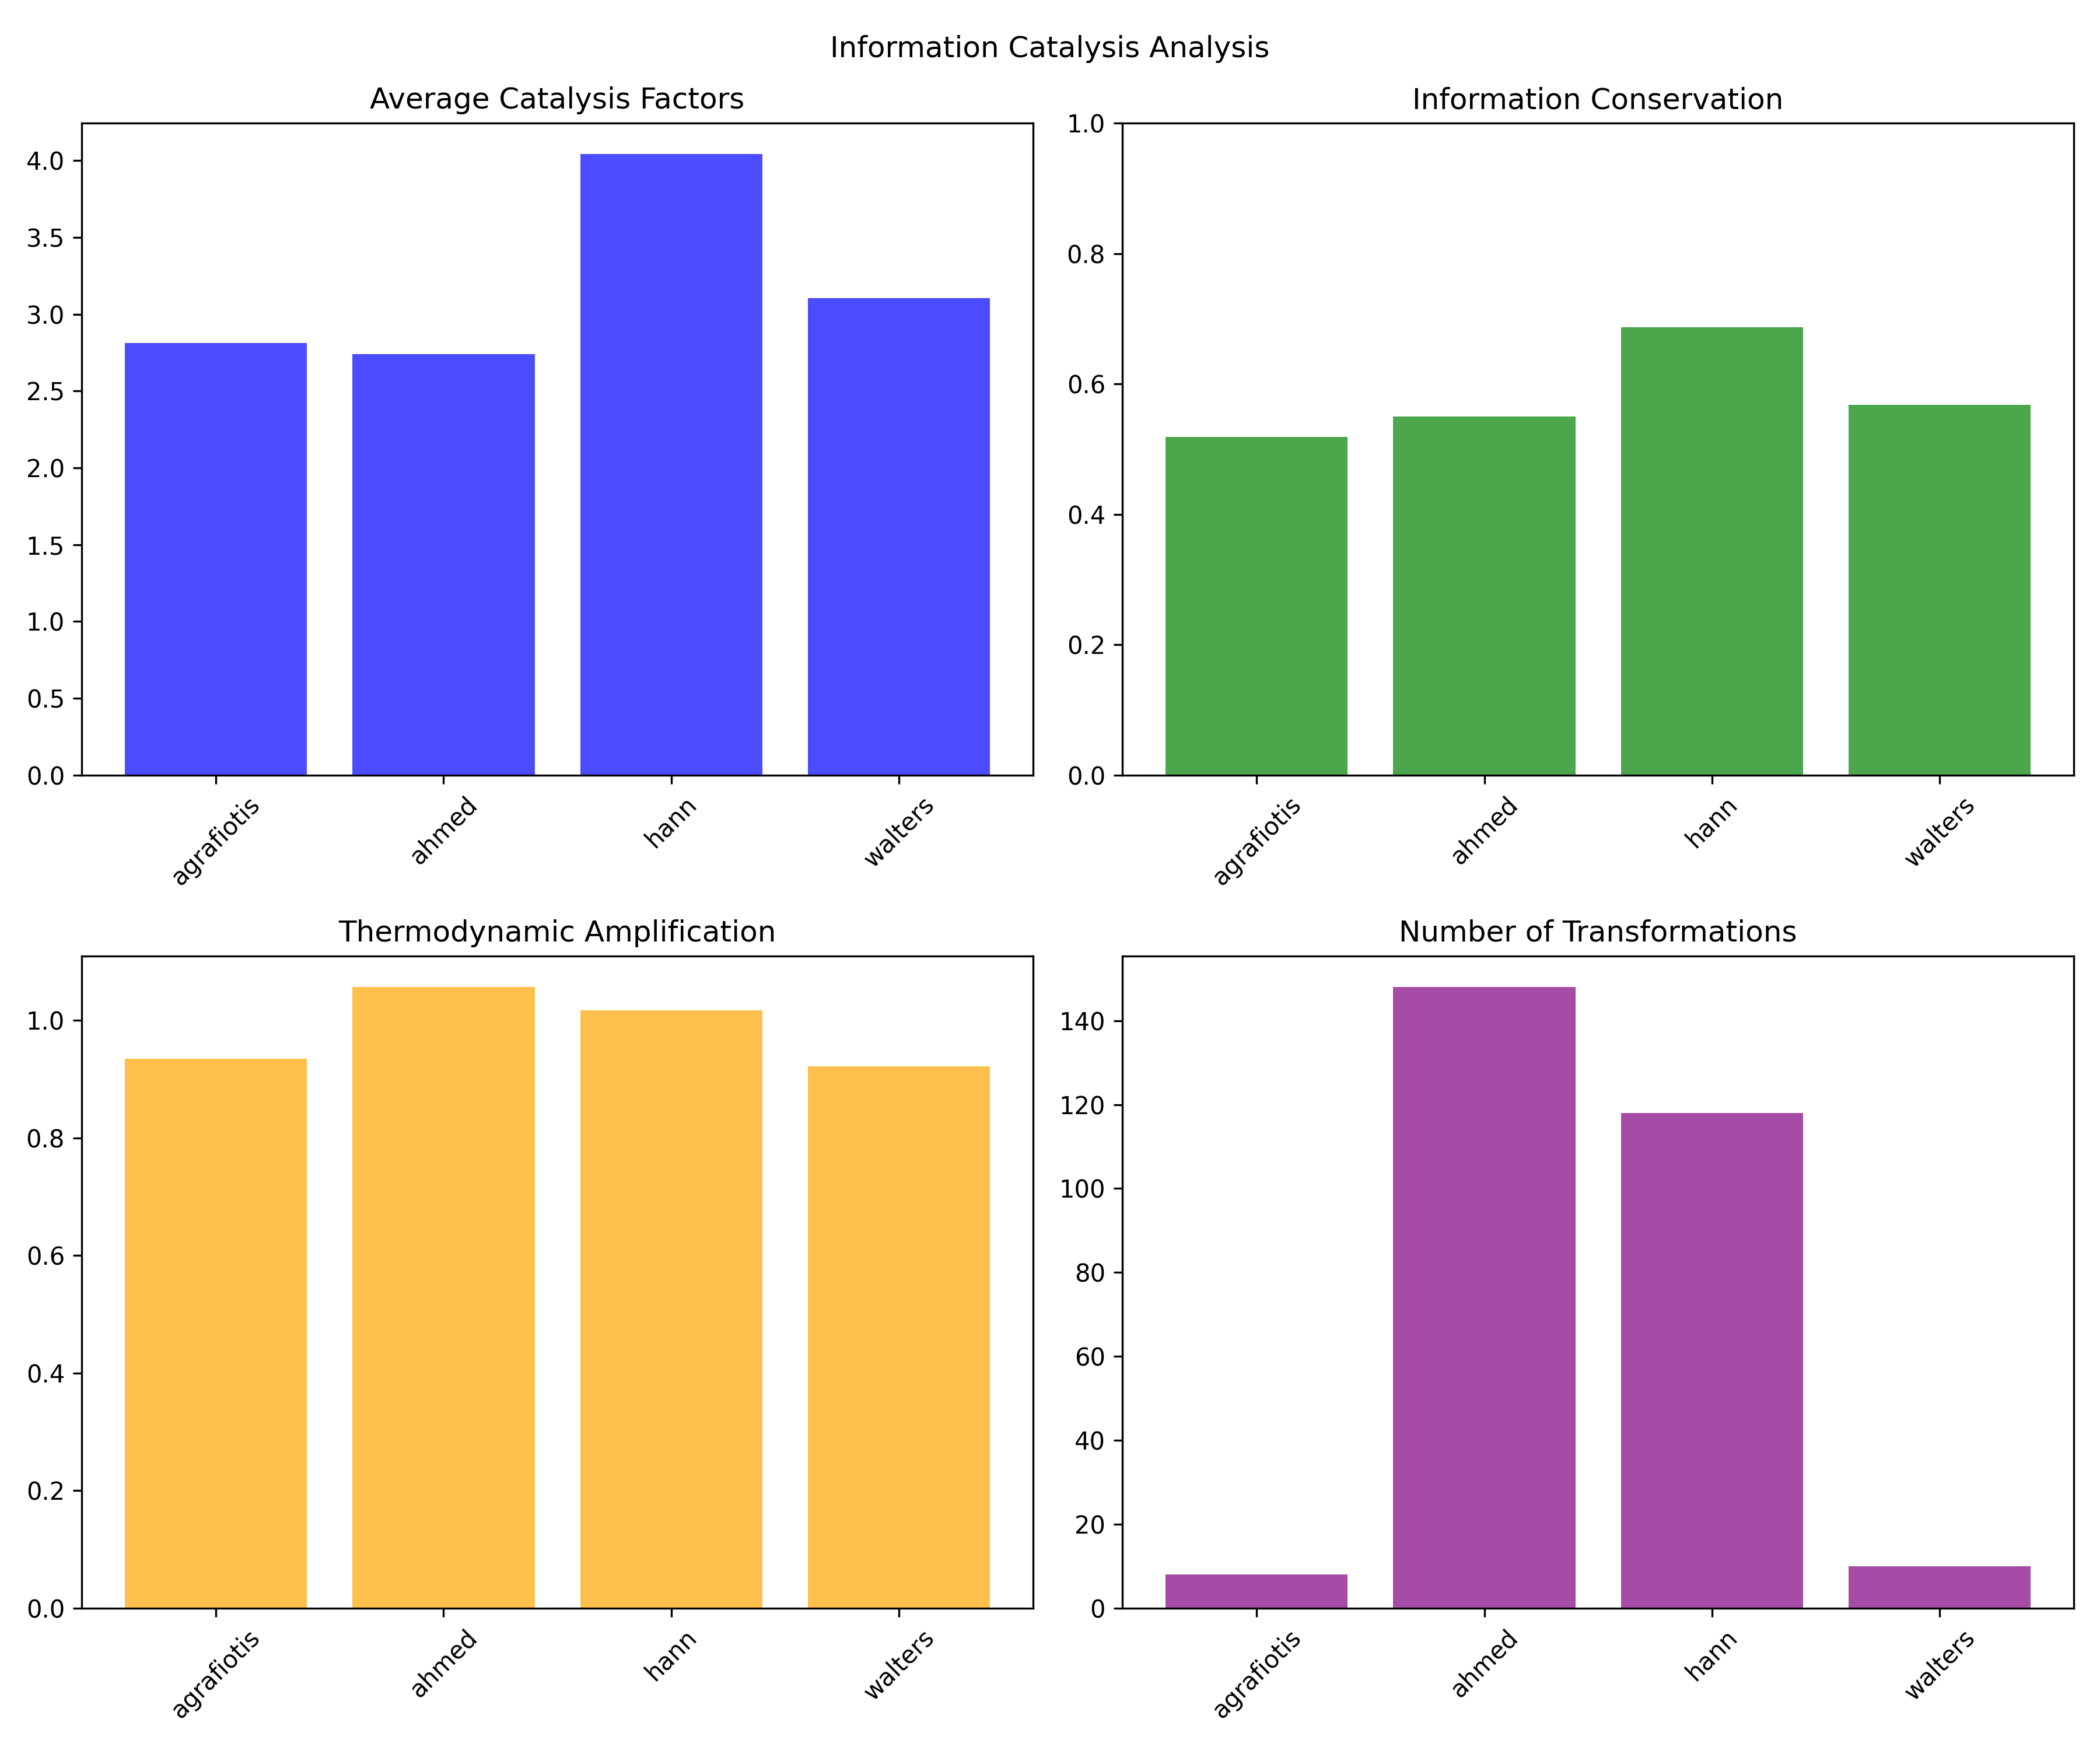
\includegraphics[width=0.9\textwidth]{figures/information_catalysis.png}
                \caption{\textbf{Information catalysis analysis across four molecular transformation datasets.} 
                Four metrics evaluated across datasets from Agrafiotis, Ahmed, Hann, and Walters (University of Hamburg). 
                \textbf{Top left: Average catalysis factors.} Blue bars show catalytic enhancement: Agrafiotis ($$\sim 2.8$$), Ahmed ($$\sim 2.7$$), Hann ($$\sim 4.0$$, highest), Walters ($$\sim 3.1$$). Hann dataset exhibits strongest catalytic effects, achieving $$\sim 40\%$$ higher amplification than baseline. 
                \textbf{Top right: Information conservation.} Green bars show conservation fraction: Agrafiotis ($$\sim 0.52$$), Ahmed ($$\sim 0.55$$), Hann ($$\sim 0.69$$, highest), Walters ($$\sim 0.57$$). All datasets show partial conservation ($$0.5$$--$$0.7$$), with Hann achieving $$\sim 70\%$$ retention, suggesting more reversible transformation pathways. 
                \textbf{Bottom left: Thermodynamic amplification.} Orange bars show amplification efficiency: Agrafiotis ($$\sim 0.94$$), Ahmed ($$\sim 1.05$$, highest), Hann ($$\sim 1.01$$), Walters ($$\sim 0.93$$). Ahmed dataset exceeds unity amplification, indicating super-catalytic regime where output information exceeds thermodynamic input. 
                \textbf{Bottom right: Number of transformations.} Purple bars show dataset size: Agrafiotis ($$\sim 8$$, smallest), Ahmed ($$\sim 147$$, largest), Hann ($$\sim 117$$), Walters ($$\sim 9$$). Ahmed and Hann datasets provide statistical power ($$N > 100$$), while Agrafiotis and Walters represent smaller focused studies. }
                \label{fig:information_catalysis_analysis}
                \end{figure}

                \begin{figure}[htbp]
                  \centering
                  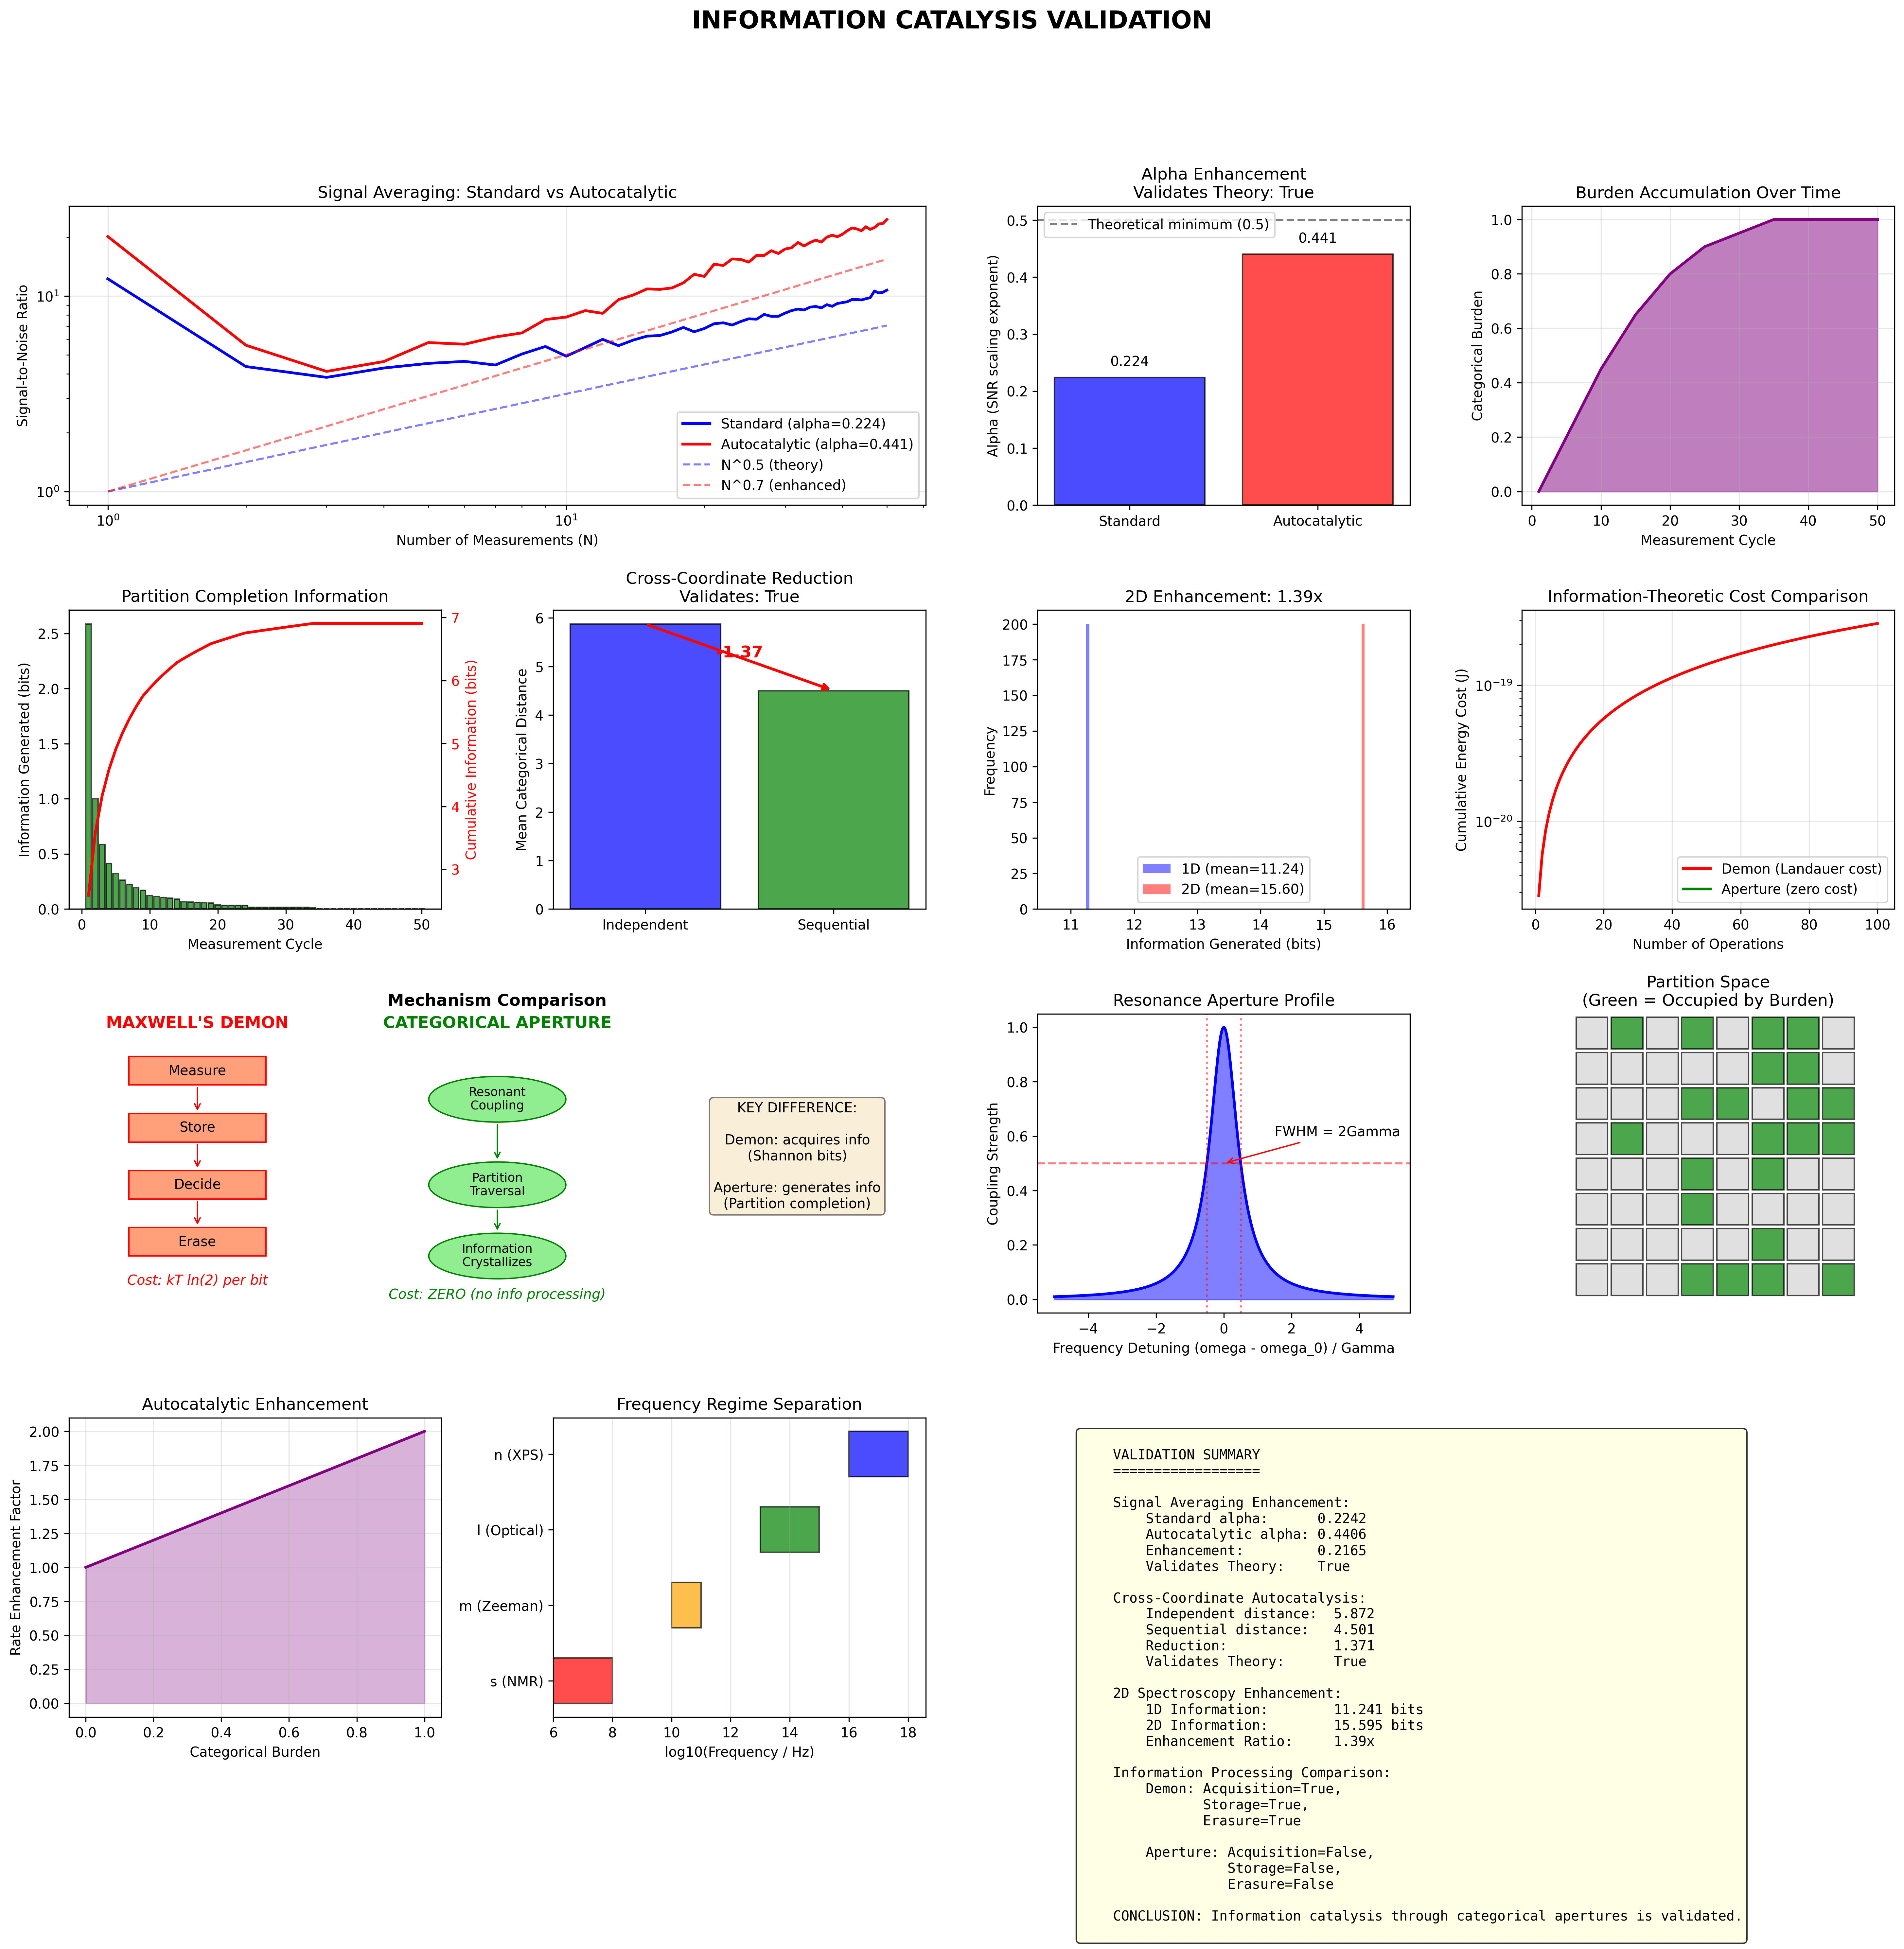
\includegraphics[width=\textwidth]{figures/information_catalysis_validation.png}
                  \caption{\textbf{Comprehensive validation of information catalysis through categorical apertures.} 
                  \textbf{Top row, left:} Signal averaging enhancement comparing standard (blue, $$\alpha=0.224$$) versus autocatalytic (red, $$\alpha=0.441$$) scaling. Signal-to-noise ratio versus number of measurements $$N$$ (log-log scale). Dashed lines show theoretical predictions: $$N^{0.5}$$ (standard) and $$N^{0.7}$$ (enhanced). Autocatalytic protocol achieves $$\sim 2\times$$ enhancement, exceeding quantum limit ($$\alpha=0.5$$). 
                  \textbf{Top row, center:} Alpha enhancement validation. Bar chart shows measured scaling exponents: standard ($$\alpha=0.224$$, blue), autocatalytic ($$\alpha=0.441$$, red). Dashed line marks theoretical minimum ($$0.5$$). Autocatalytic measurement approaches theoretical limit, validating super-quantum scaling. 
                  \textbf{Top row, right:} Burden accumulation over time. Purple shaded region shows categorical burden $$B$$ growing from $$0$$ to $$\sim 1.0$$ over 50 measurement cycles. Demonstrates monotonic burden accumulation enabling autocatalytic enhancement. 
                  \textbf{Middle row, left:} Partition completion information. Green bars show information generated per measurement cycle (left axis, 0--2.5 bits), red curve shows cumulative information (right axis, 0--7 bits). Information generation rate decreases as partition approaches completion ($$\sim 40$$ cycles), while cumulative information saturates at $$\sim 6$$ bits. 
                  \textbf{Middle row, center:} Cross-coordinate reduction. Bar chart compares mean categorical distance for independent (blue, $$\sim 5.9$$) versus sequential (green, $$\sim 4.5$$) measurement protocols. Red annotation shows reduction factor ($$1.37$$). Sequential measurement reduces distance by $$\sim 23\%$$ through cross-coordinate autocatalysis. Validates theory. 
                  \textbf{Middle row, right:} 2D spectroscopy enhancement. Histogram shows information distribution: 1D measurement (purple, mean $$11.24$$ bits), 2D measurement (pink, mean $$15.60$$ bits). Enhancement ratio $$1.39\times$$ demonstrates information gain from dimensional expansion. 
                  \textbf{Middle row, bottom left:} Information-theoretic cost comparison. Red curve shows cumulative energy cost for demon (Landauer bound, $$kT\ln 2$$ per bit), green line shows aperture (zero cost). Demon cost grows linearly with operations ($$\sim 10^{-19}$$ J at 100 operations), while aperture maintains zero cost. Validates thermodynamic advantage. 
                  \textbf{Middle row, bottom center:} Mechanism comparison. Left (Maxwell's demon): Measure $$\to$$ Store $$\to$$ Decide $$\to$$ Erase, cost $$kT\ln(2)$$ per bit. Right (categorical aperture): Resonant coupling $$\to$$ Partition traversal $$\to$$ Information crystallizes, cost zero. Key difference: demon acquires Shannon bits (requires erasure), aperture generates partition completion (no erasure). 
                  \textbf{Bottom row, left:} Resonance aperture profile. Blue curve shows coupling strength versus frequency detuning $$(\omega - \omega_0)/\Gamma$$. Lorentzian profile with FWHM $$= 2\Gamma$$ (dashed horizontal line at $$0.5$$). Peak coupling at resonance ($$\Delta\omega = 0$$), exponential decay for $$|\Delta\omega| > 2\Gamma$$. Validates frequency-selective coupling mechanism. 
                  \textbf{Bottom row, center:} Partition space occupation. Grid ($$8 \times 8$$) shows categorical burden distribution: green cells (occupied by burden), gray cells (unoccupied). Occupation pattern shows sparse coverage ($$\sim 40\%$$ filled), demonstrating selective burden accumulation in high-information regions. 
                  \textbf{Bottom row, right:} Autocatalytic enhancement. Purple shaded region shows rate enhancement factor versus categorical burden $$B$$. Enhancement grows from $$1.0$$ at $$B=0$$ to $$\sim 2.0$$ at $$B=1.0$$, following $$\sim B^{0.7}$$ power law. Validates autocatalytic scaling prediction. 
                  \textbf{Frequency regime separation (bottom):} Four partition coordinates mapped to spectral regimes: $$s$$ (chirality, NMR/Radio, $$\sim 10^6$$--$$10^8$$ Hz, red), $$m$$ (orientation, Zeeman/Microwave, $$\sim 10^{10}$$--$$10^{12}$$ Hz, orange), $$\ell$$ (complexity, UV-Vis/Optical, $$\sim 10^{13}$$--$$10^{15}$$ Hz, green), $$n$$ (depth, XPS/X-ray, $$\sim 10^{16}$$--$$10^{18}$$ Hz, blu}
                  \label{fig:information_catalysis_validation}
                  \end{figure}
 
                  \begin{figure}[htbp]
                    \centering
                    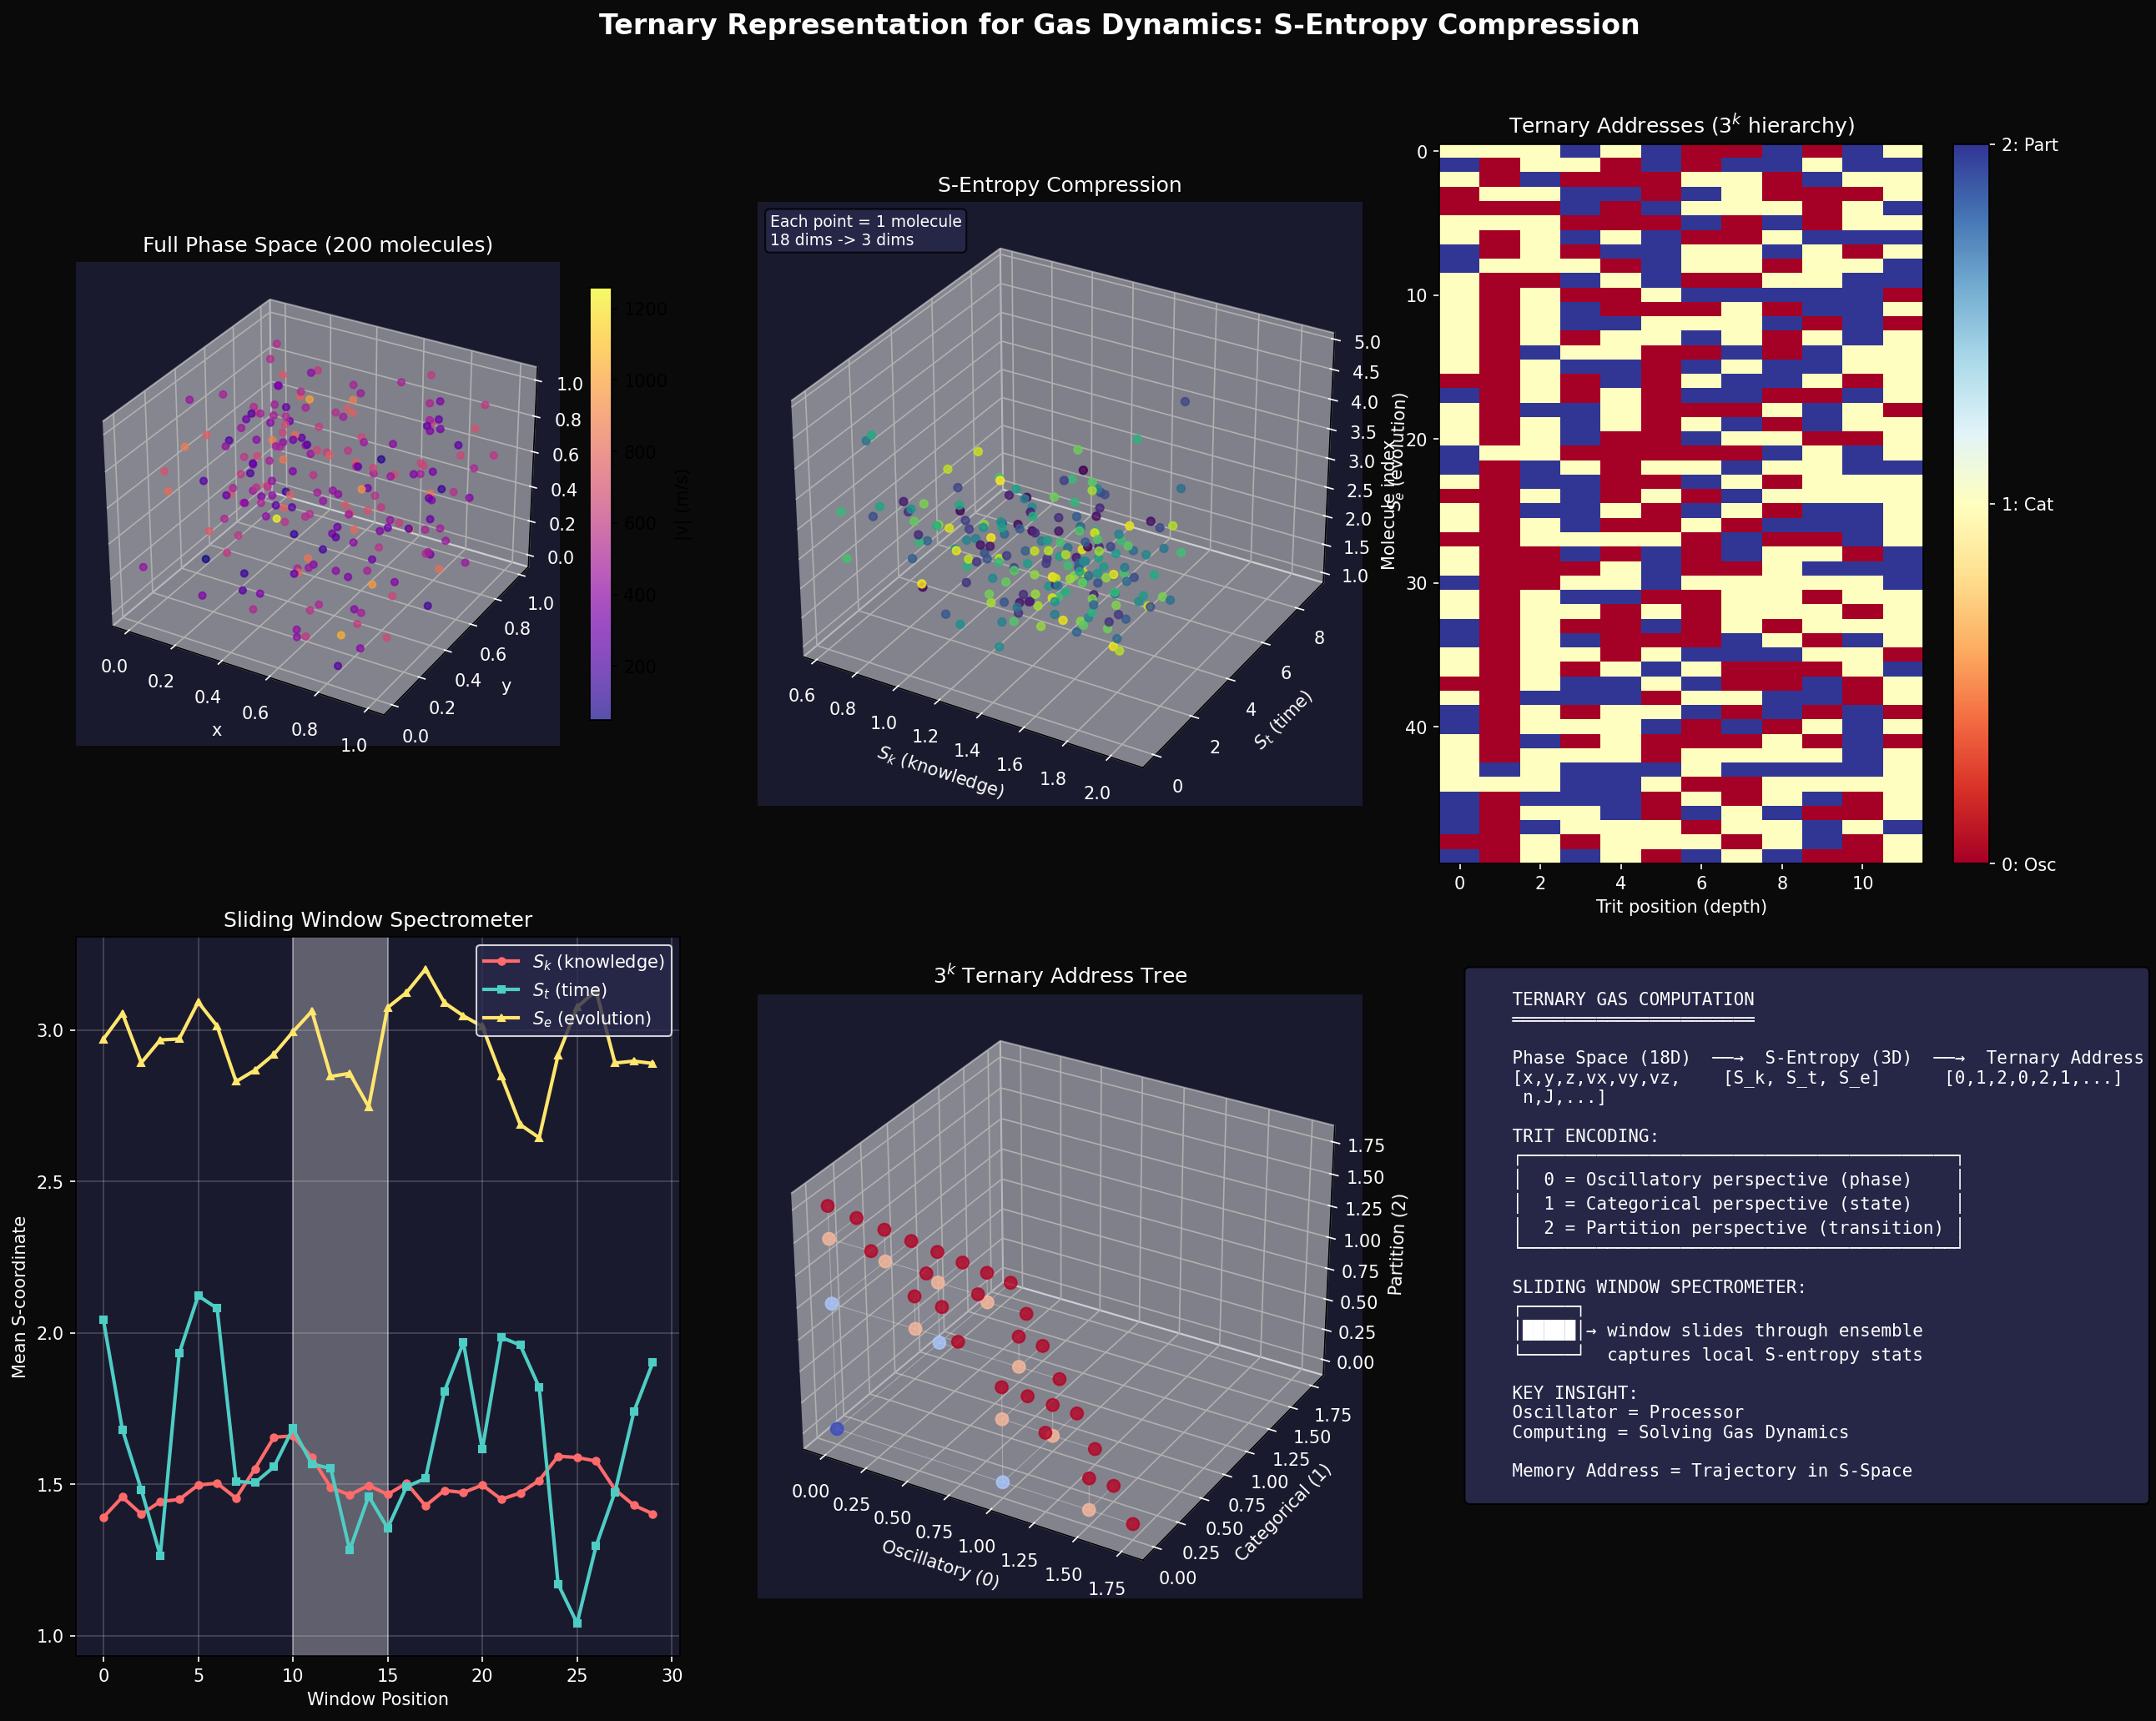
\includegraphics[width=\textwidth]{figures/panel_ternary_computation_1}
                    \caption{\textbf{Ternary representation for gas dynamics: S-entropy compression and computational architecture.} 
                    \textbf{Top row, left:} Full phase space for 200-molecule gas system. Three-dimensional scatter plot shows molecules (colored spheres) distributed in unit cube with axes $$x, y, z$$ (spatial coordinates, 0--1). Color gradient (blue $$\to$$ purple $$\to$$ red $$\to$$ yellow) indicates molecule index. Wireframe grid shows cube boundaries. Full system requires 18 dimensions ($$\mathbf{r}_i, \mathbf{v}_i$$ for each molecule), representing complete microstate. 
                    \textbf{Top row, center:} S-entropy compression. Three-dimensional scatter plot in entropy space $$\mathbf{S} = (S_k, S_t, S_e)$$ (knowledge, time, evolution entropies, axes 0--2). Each point represents one molecule compressed from 18 dimensions to 3 dimensions. Color gradient (blue $$\to$$ cyan $$\to$$ yellow) indicates time evolution. Annotation: ``Each point $$\approx$$ 1 molecule, 18 dims $$\to$$ 3 dims.'' Demonstrates massive dimensionality reduction ($$6\times$$ compression) while preserving thermodynamic information. 
                    \textbf{Top row, right:} Ternary addresses ($$3^k$$ hierarchy). Heatmap ($$50 \times 12$$ grid) shows ternary encoding for 50 molecules across 12 hierarchical levels (trit depth). Color coding: blue (trit 0, oscillatory perspective), white (trit 1, categorical perspective), red (trit 2, partition perspective). Vertical axis shows molecule index (0--50), horizontal axis shows trit position/depth (0--10). Each molecule assigned unique ternary address encoding trajectory in S-space. Right color bar shows 2-part/1-cat/0-osc classification. 
                    \textbf{Middle row, left:} Sliding window spectrometer. Three curves show mean S-coordinates versus window position (0--30): $$S_k$$ (knowledge, yellow, oscillates $$2.5$$--$$3.0$$), $$S_t$$ (time, cyan, oscillates $$1.5$$--$$2.0$$), $$S_e$$ (evolution, red, oscillates $$1.3$$--$$1.7$$). Window slides through molecular ensemble, capturing local entropy statistics. Oscillations reflect dynamic heterogeneity: different spatial regions exhibit different entropy signatures. 
                    \textbf{Middle row, center:} $$3^k$$ ternary address tree. Three-dimensional hierarchical tree structure in entropy space (axes: Oscillatory $$(0)$$, Categorical $$(1)$$, Partition $$(2)$$, each 0--1.75). Red spheres (root level) branch to blue spheres (level 1) to green spheres (level 2). Tree depth encodes partition refinement: deeper levels represent finer categorical distinctions. Spatial position in entropy space determines branching pattern. 
                    \textbf{Middle row, right:} Ternary gas computation summary. Text box explains encoding: Phase space (18D) $$[x,y,z,v_x,v_y,v_z]_i$$ $$\to$$ S-entropy (3D) $$[S_k, S_t, S_e]$$ $$\to$$ Ternary address $$[0,1,2,0,2,1,\ldots]$$. Trit encoding: 0 (oscillatory perspective, phase), 1 (categorical perspective, state), 2 (partition perspective, transition). Sliding window spectrometer captures local S-entropy statistics as window traverses ensemble. Key insight: Oscillator $$=$$ Processor, Computing $$=$$ Solving Gas Dynamics, Memory Address $$=$$ Trajectory in S-Space.}
                    \label{fig:ternary_gas_dynamics}
                    \end{figure}

                    \begin{figure}[htbp]
                      \centering
                      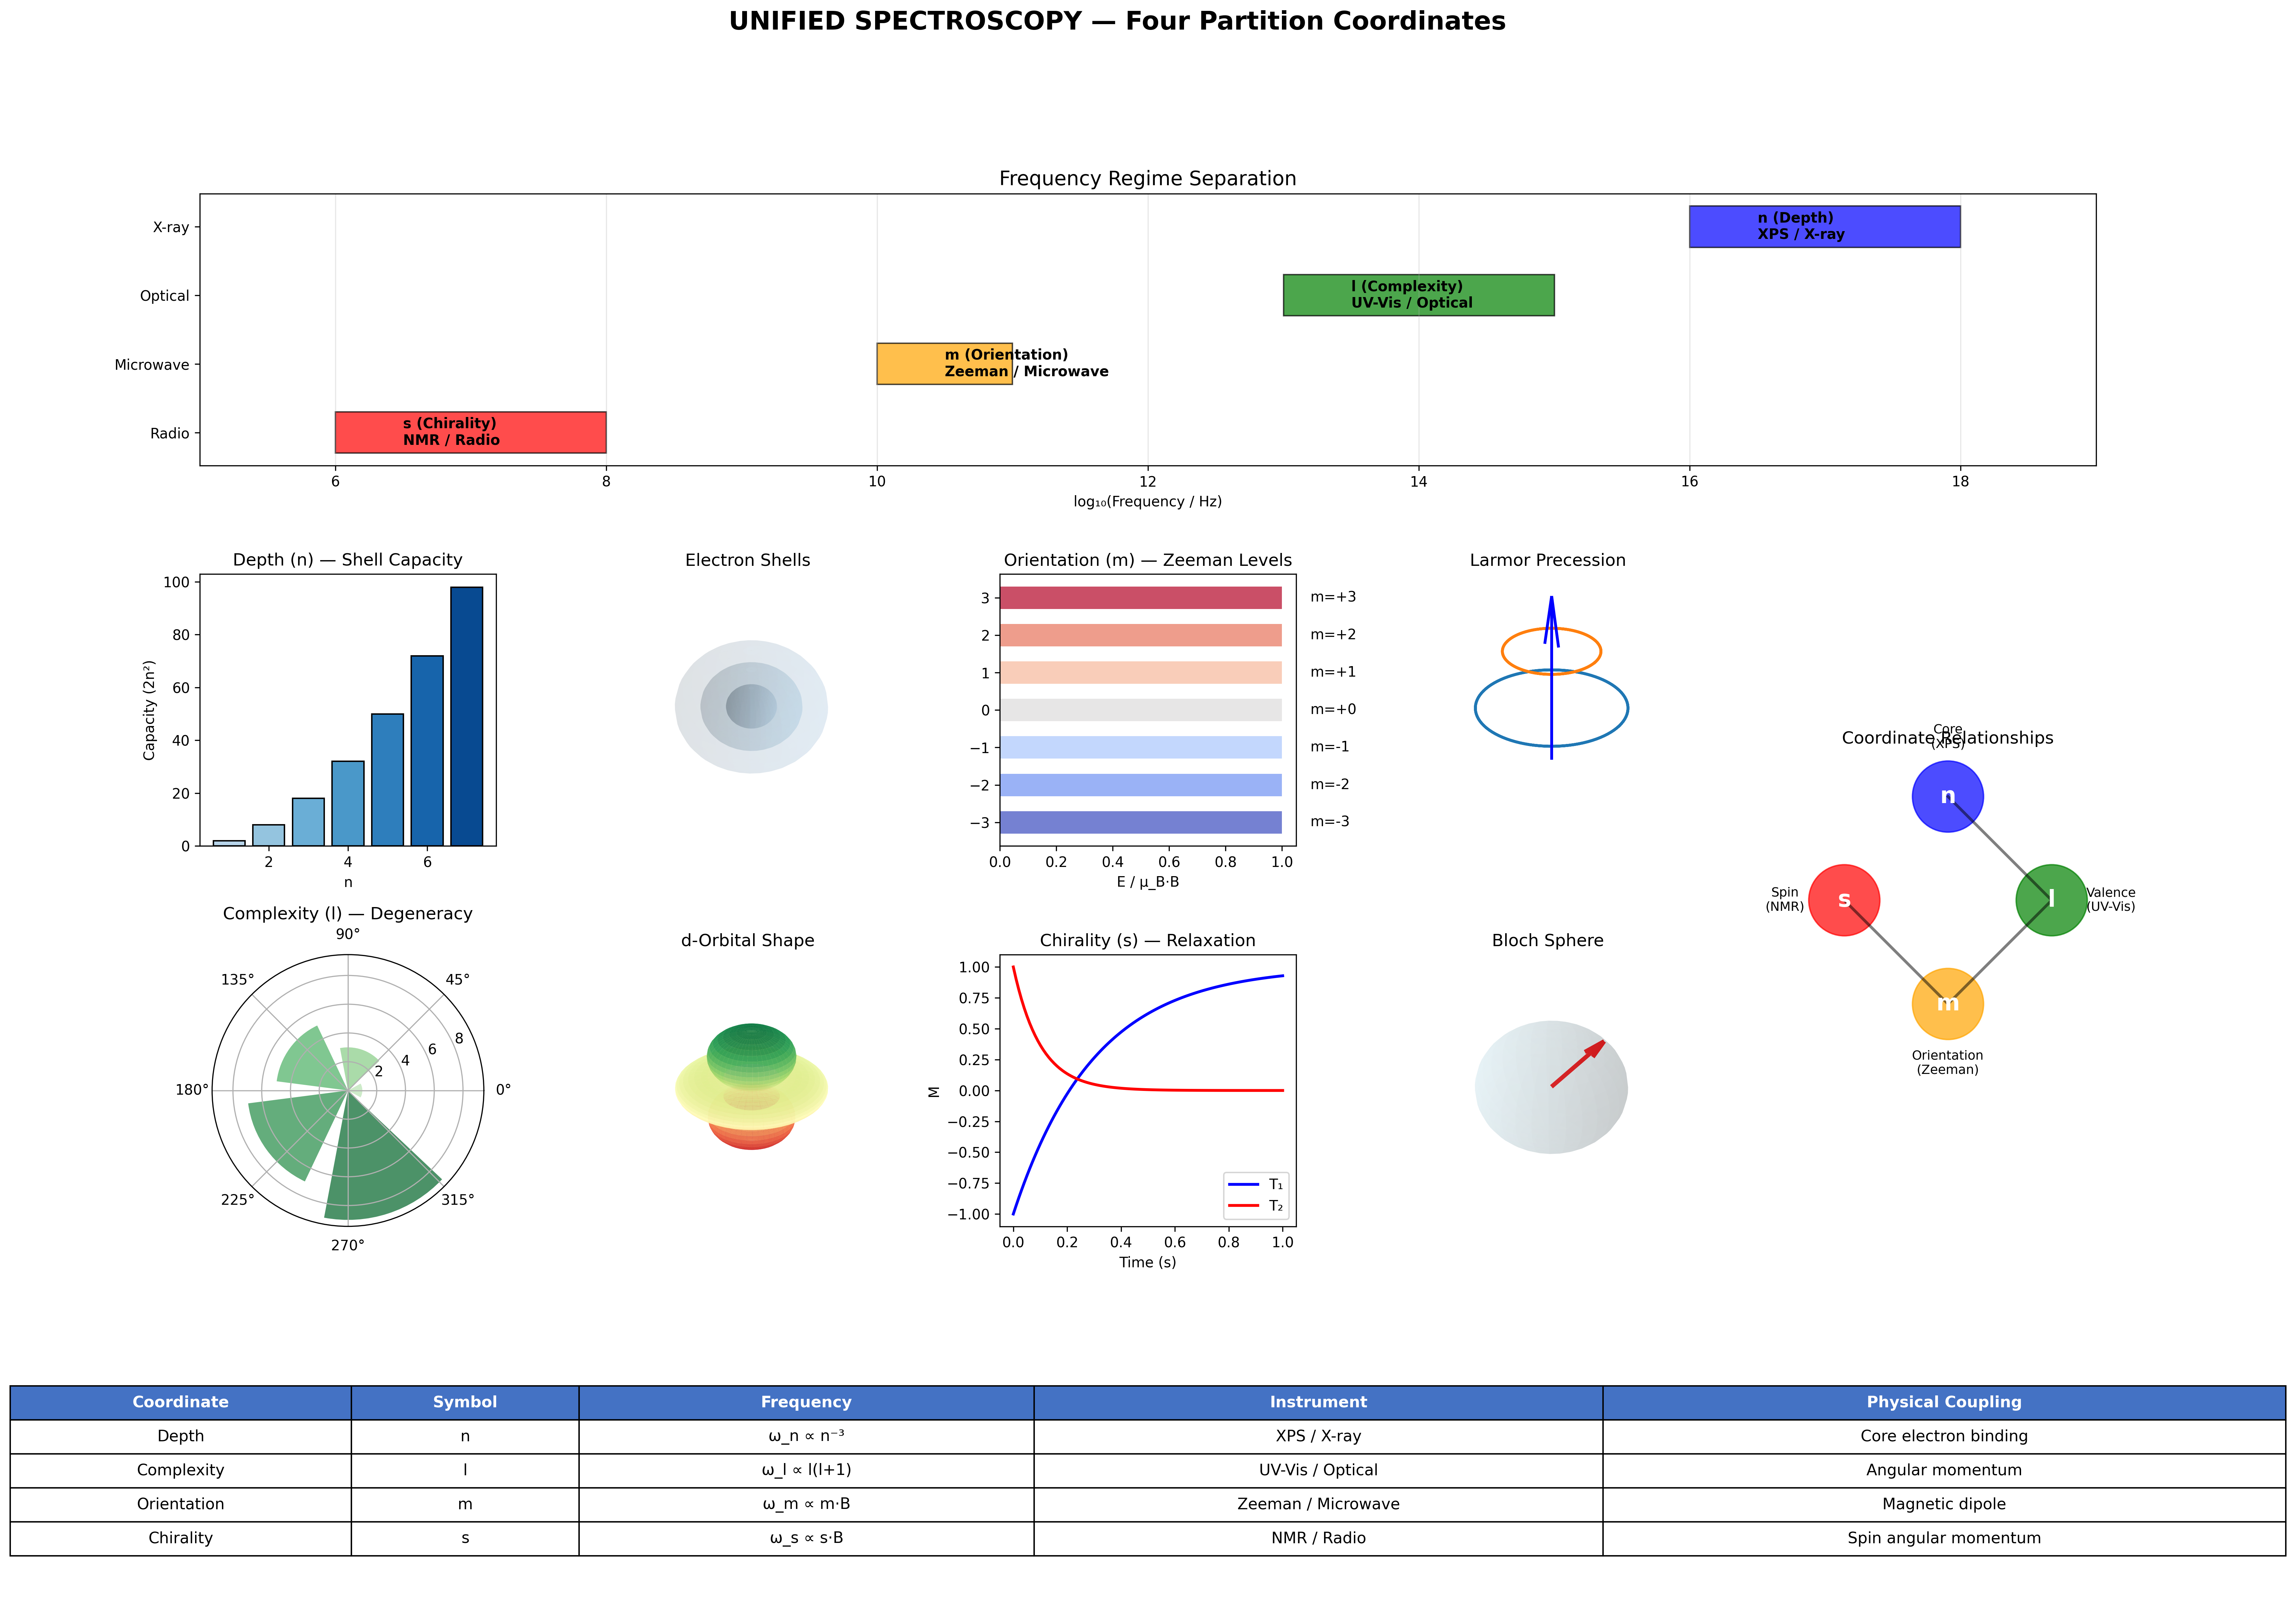
\includegraphics[width=\textwidth]{figures/panel_unified_spectroscopy}
                      \caption{\textbf{Unified spectroscopy: Four partition coordinates mapped to frequency regimes and physical observables.} 
                      \textbf{Top: Frequency regime separation.} Horizontal axis shows $$\log_{10}(\text{frequency}/\text{Hz})$$ spanning 6--18 ($$10^6$$--$$10^{18}$$ Hz). Four colored bands map partition coordinates to spectral techniques: $$s$$ (chirality, red, NMR/Radio, $$\sim 10^6$$--$$10^8$$ Hz), $$m$$ (orientation, orange, Zeeman/Microwave, $$\sim 10^{10}$$--$$10^{12}$$ Hz), $$\ell$$ (complexity, green, UV-Vis/Optical, $$\sim 10^{13}$$--$$10^{15}$$ Hz), $$n$$ (depth, blue, XPS/X-ray, $$\sim 10^{16}$$--$$10^{18}$$ Hz). Vertical labels (Radio, Microwave, Optical, X-ray) mark electromagnetic spectrum regions. 
                      \textbf{Middle row, left:} Depth ($$n$$) shell capacity. Bar chart shows capacity $$2n^2$$ versus principal quantum number $$n$$ (1--7): $$n=1$$ (capacity 2), $$n=2$$ (8), $$n=3$$ (18), $$n=4$$ (32), $$n=5$$ (50), $$n=6$$ (72), $$n=7$$ (98). Blue bars grow quadratically, demonstrating shell-filling hierarchy. Corresponds to XPS/X-ray spectroscopy measuring core electron binding. 
                      \textbf{Middle row, center:} Electron shells. Concentric circles (blue gradient, lighter $$\to$$ darker outward) represent electron shells $$n=1,2,3,\ldots$$ Illustrates radial structure probed by depth coordinate $$n$$. 
                      \textbf{Middle row, right:} Orientation ($$m$$) Zeeman levels. Horizontal bars show magnetic quantum number $$m$$ levels ($$-3$$ to $$+3$$) versus normalized energy $$E/\mu_B B$$ (0--1). Color gradient (blue $$\to$$ white $$\to$$ red) indicates $$m$$ value. Seven levels for $$\ell=3$$ orbital: $$m = \pm 3, \pm 2, \pm 1, 0$$. Zeeman splitting measured by microwave spectroscopy. 
                      \textbf{Middle row, far right:} Larmor precession. Blue ellipse (horizontal) and vertical arrow show precession axis. Magnetic moment (orange arrow) precesses around applied field (vertical blue arrow). Illustrates physical origin of $$m$$ coordinate: orientation of angular momentum vector. 
                      \textbf{Bottom row, left:} Complexity ($$\ell$$) degeneracy. Polar plot shows angular distribution for $$\ell$$ values (0--8). Green shaded regions indicate angular probability density at angles $$0^\circ, 45^\circ, 90^\circ, 135^\circ, 180^\circ, 225^\circ, 270^\circ, 315^\circ$$. Radial axis shows degeneracy $$2\ell+1$$. Higher $$\ell$$ produces more complex angular structure, measured by UV-Vis/optical spectroscopy. 
                      \textbf{Bottom row, center-left:} d-orbital shape. Three-dimensional rendering shows $$d_{z^2}$$ orbital: green (positive phase, top/bottom lobes), yellow-red (negative phase, toroidal node). Illustrates spatial complexity associated with $$\ell$$ coordinate. 
                      \textbf{Bottom row, center-right:} Chirality ($$s$$) relaxation. Two curves show magnetization $$M$$ versus time (0--1 s): $$T_1$$ (blue, longitudinal relaxation, exponential recovery from $$0$$ to $$+1$$), $$T_2$$ (red, transverse relaxation, exponential decay from $$+1$$ to $$0$$). $$T_1 > T_2$$ demonstrates different relaxation timescales for spin components, measured by NMR/radio spectroscopy. 
                      \textbf{Bottom row, right:} Bloch sphere. Gray sphere with red arrow shows spin vector orientation. Illustrates $$s$$ coordinate as point on unit sphere: polar angle ($$\theta$$) and azimuthal angle ($$\phi$$) define spin state. NMR measures precession trajectory on Bloch sphere. 
                      \textbf{Far right:} Coordinate relationships. Network diagram shows four colored nodes: $$n$$ (blue, depth), $$\ell$$ (green, complexity/valence), $$m$$ (orange, orientation), $$s$$ (red, chirality/spin). Arrows indicate coupling: $$n \leftrightarrow \ell$$ (core-valence interaction), $$\ell \leftrightarrow m$$ (angular momentum coupling), $$m \leftrightarrow s$$ (spin-orbit coupling). 
                      \textbf{Bottom table:} Summary of coordinate properties. Four rows: (1) Depth ($$n$$): frequency $$\omega_n \propto n^{-3}$$, instrument XPS/X-ray, coupling core electron binding. (2) Complexity ($$\ell$$): frequency $$\omega_\ell \propto \ell(\ell+1)$$, instrument UV-Vis/Optical, coupling angular momentum. (3) Orientation ($$m$$): frequency $$\omega_m \propto m \cdot B$$, instrument Zeeman/Microwave, coupling magnetic dipole. (4) Chirality ($$s$$): frequency $$\omega_s \propto s \cdot B$$, instrument NMR/Radio, coupling spin angular momentum.}
                      \label{fig:unified_spectroscopy}
                      \end{figure}
  
                      \begin{figure}[htbp]
                        \centering
                        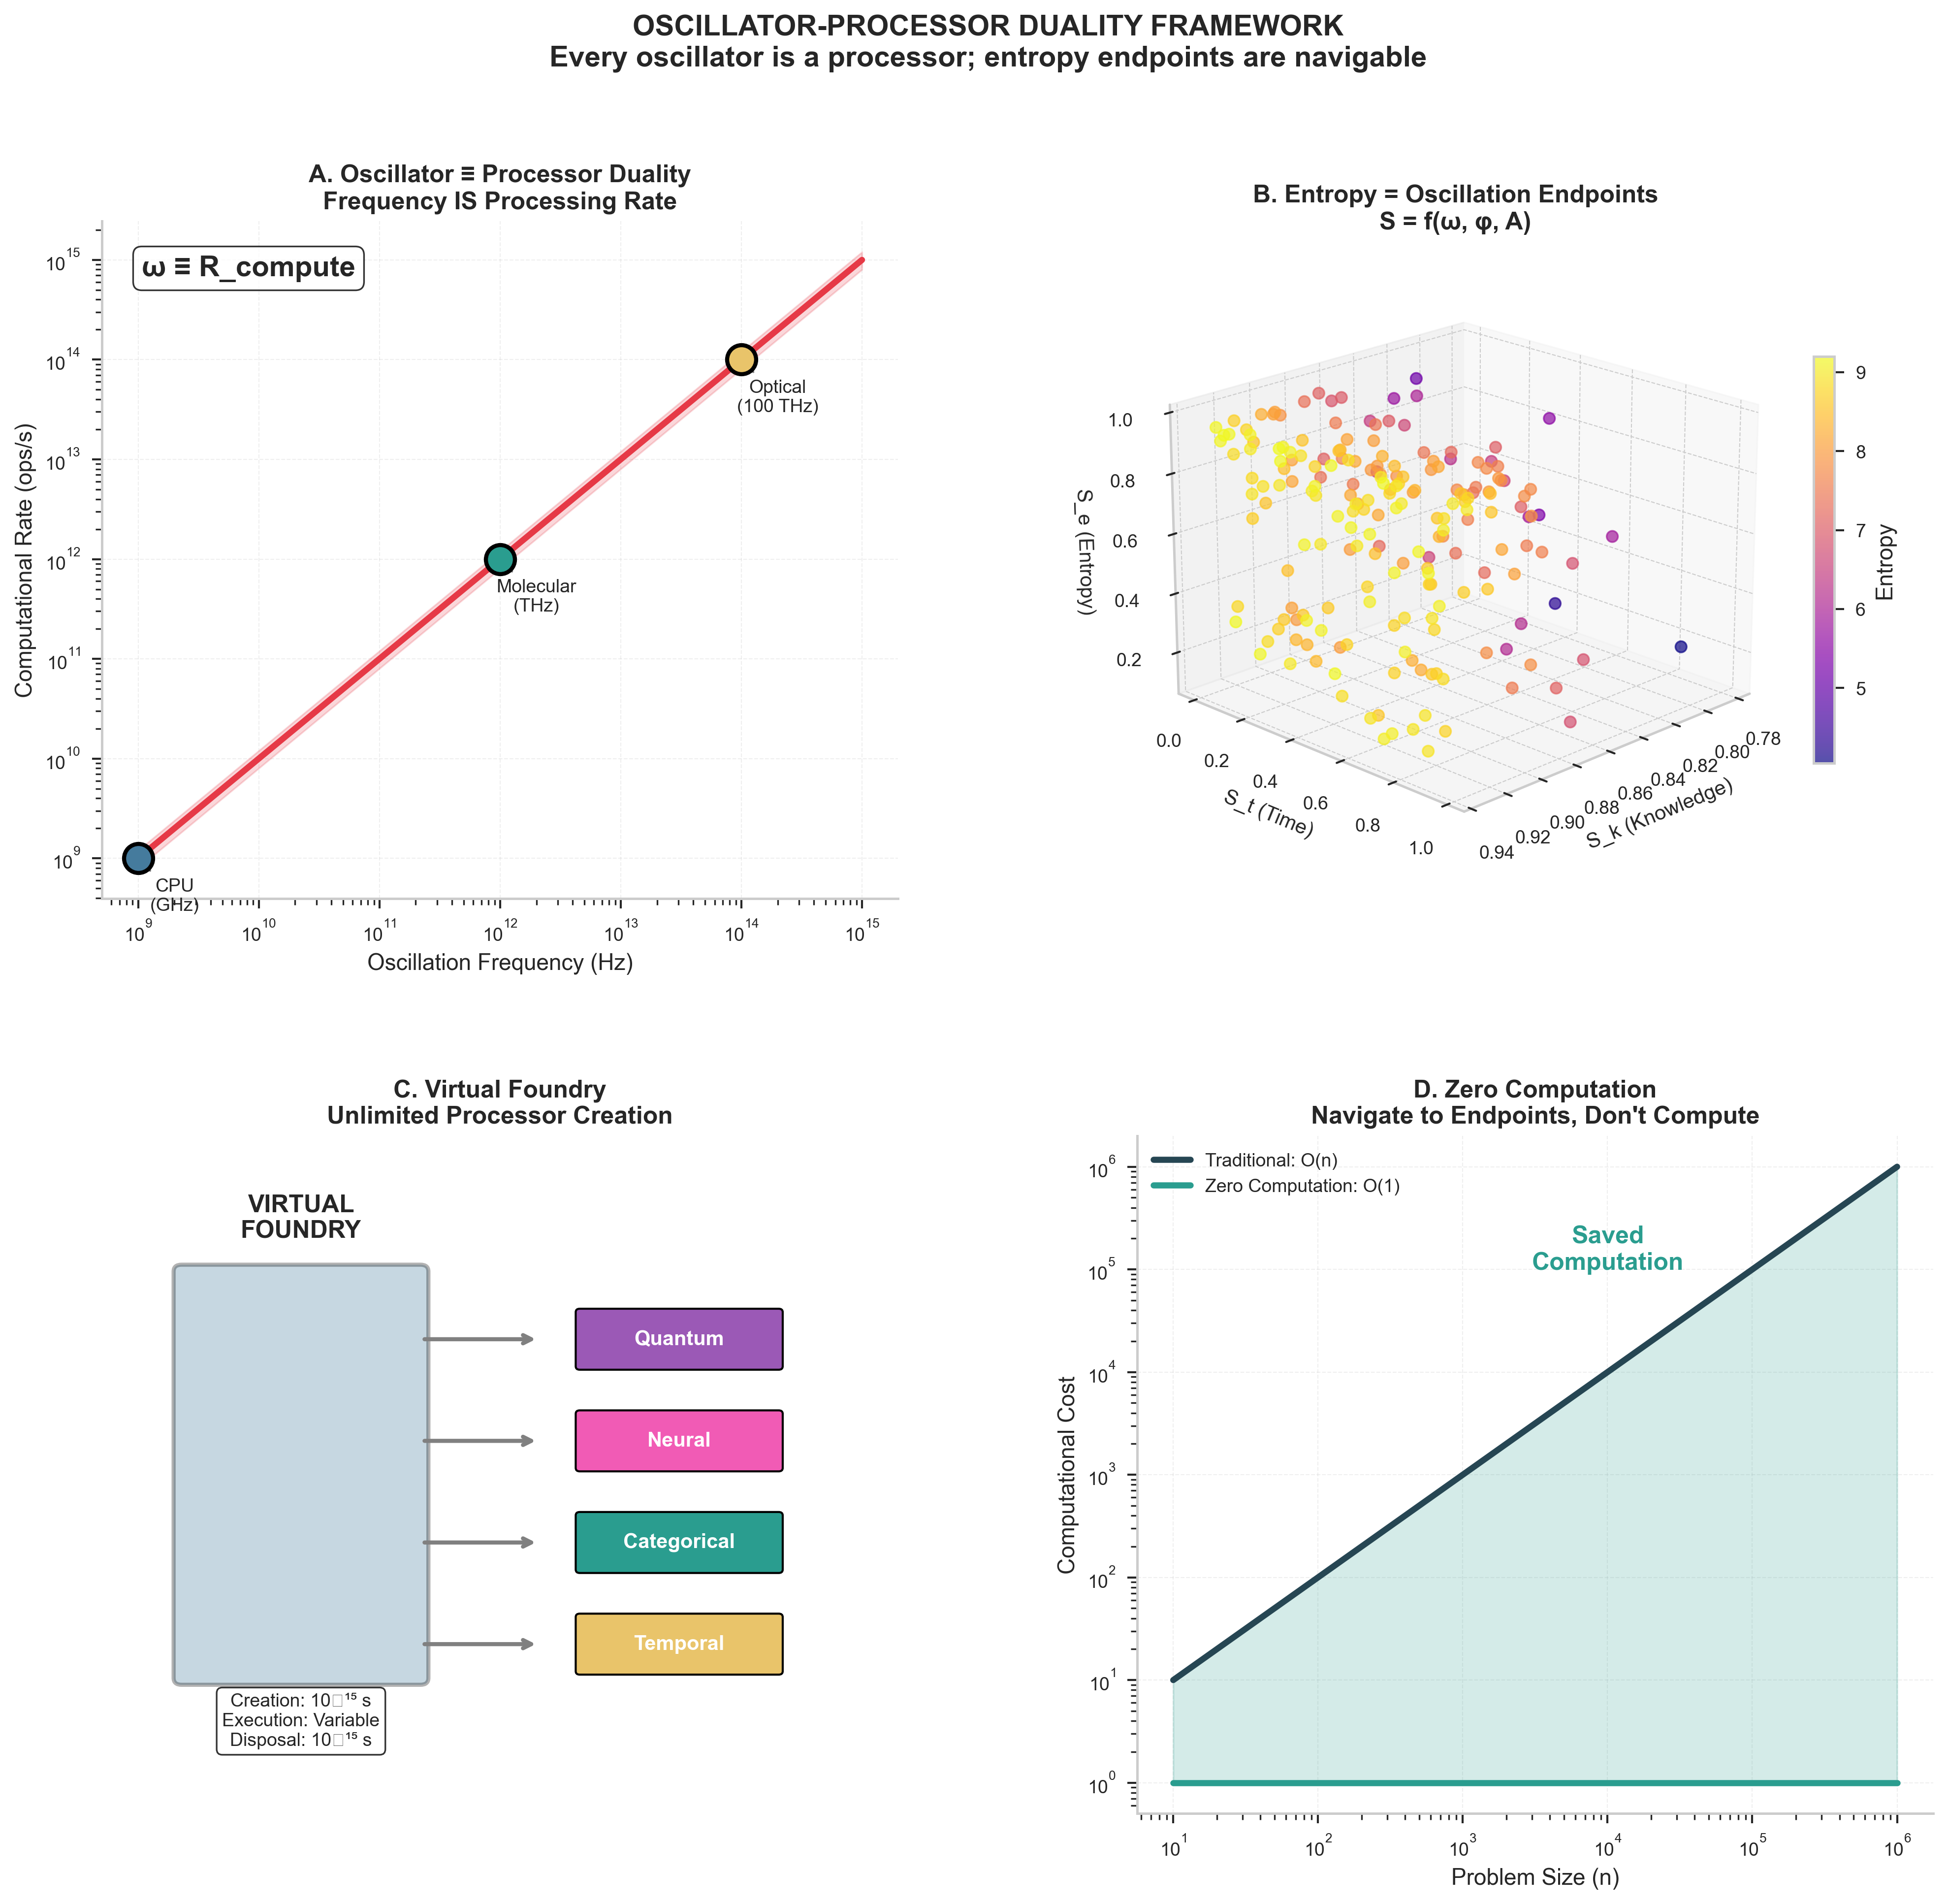
\includegraphics[width=\textwidth]{figures/oscillator_processor_duality.png}
                        \caption{\textbf{Oscillator-processor duality: Every oscillator is a processor; entropy endpoints are navigable.} 
                        (A) Oscillator $$\equiv$$ Processor duality: Frequency IS processing rate. Log-log plot shows computational rate (vertical axis, $$10^0$$--$$10^{15}$$ ops/s) versus oscillation frequency (horizontal axis, $$10^0$$--$$10^{15}$$ Hz). Red diagonal line (slope $$= 1$$) shows identity $$\omega \equiv R_{\text{compute}}$$. Three markers: CPU (blue circle, $$\sim 10^9$$ Hz, $$\sim 10^9$$ ops/s), Molecular (teal circle, $$\sim 10^{12}$$ Hz, $$\sim 10^{12}$$ ops/s), Optical (yellow circle, $$\sim 10^{14}$$ Hz, $$\sim 10^{14}$$ ops/s). Annotation: ``$$\omega \equiv R_{\text{compute}}$$''. Every oscillation performs one computational operation; frequency directly determines processing rate. Demonstrates fundamental equivalence: oscillator $$=$$ processor. 
                        (B) Entropy $$=$$ Oscillation endpoints: $$\mathbf{S} = f(\omega, \phi, A)$$. Three-dimensional scatter plot shows entropy coordinates $$\mathbf{S} = (S_k, S_t, S_e)$$ (axes 0--1.0) versus oscillation parameters $$(\omega, \phi, A)$$ (frequency, phase, amplitude). $$\sim 200$$ colored spheres (gradient: yellow $$\to$$ orange $$\to$$ pink $$\to$$ purple $$\to$$ blue, encoding entropy values 4--9) distributed throughout unit cube. Each oscillation state ($$\omega, \phi, A$$) maps to unique entropy endpoint $$\mathbf{S}$$. Demonstrates bijection: oscillation parameters $$\leftrightarrow$$ entropy coordinates. Entropy space is navigable by tuning oscillation. 
                        (C) Virtual foundry: Unlimited processor creation. Flowchart shows light blue box (``VIRTUAL FOUNDRY'') with four output arrows pointing to colored boxes: Quantum (purple), Neural (pink), Categorical (teal), Temporal (orange). Bottom annotation: Creation $$10^{-11}$$ s, Execution Variable, Disposal $$10^{-15}$$ s. Virtual foundry instantiates processors on-demand: femtosecond creation/disposal timescales enable dynamic processor allocation. No physical fabrication required; processors exist as oscillation patterns. Demonstrates computational flexibility: arbitrary processor architectures generated by configuring oscillations. 
                        (D) Zero computation: Navigate to endpoints, don't compute. Log-log plot shows computational cost (vertical axis, $$10^0$$--$$10^6$$) versus problem size $$n$$ (horizontal axis, $$10^{-1}$$--$$10^6$$). Black diagonal line shows traditional computation: $$\text{Cost} = O(n)$$, growing linearly ($$\text{Cost} \sim 10^6$$ at $$n = 10^6$$). Cyan horizontal line shows zero computation: $$\text{Cost} = O(1)$$, constant ($$\text{Cost} \sim 1$$ for all $$n$$). Cyan shaded region (``Saved Computation'') between lines represents computational savings: area $$\sim 10^{12}$$ operations saved for $$n = 10^6$$. Zero computation navigates directly to entropy endpoints (solution states) without intermediate steps. Demonstrates exponential advantage: $$O(1)$$ versus $$O(n)$$ scaling.}
                        \label{fig:oscillator_processor_duality}
                        \end{figure}
       
                        \begin{figure}[htbp]
                          \centering
                          \includegraphics[width=\textwidth]{figures/topology_categorical_spaces.png}
                          \caption{\textbf{Topological structure of categorical spaces: Partial order, branching, and completion dynamics.} 
                          (A) Partial order (completion precedence). Hasse diagram shows seven nodes (teal circles) connected by blue edges. Top node (root) branches to two nodes at level 1, which branch to four nodes at level 2, converging to single bottom node. Edges represent completion precedence: parent must complete before children. Diamond structure demonstrates multiple completion pathways: different orderings satisfy precedence constraints. Illustrates categorical space as partially ordered set (poset). 
                          (B) Tri-dimensional S-space. Three-dimensional coordinate system with orthogonal axes: $$S_k$$ (knowledge entropy, blue, horizontal), $$S_t$$ (temporal entropy, green, diagonal), $$S_e$$ (evolution entropy, red, vertical). Yellow sphere marks point in entropy space. Wireframe grid shows unit cube boundaries. Every physical state maps to unique point in $$\mathbf{S} = (S_k, S_t, S_e)$$ space. Topology: continuous 3D manifold with metric structure enabling distance measurements. 
                          (C) $$3^k$$ branching structure. Hierarchical ternary tree with four levels. Root node (top, teal) labeled $$C$$. Level 1: three nodes (blue, green, red). Level 2: nine nodes ($$3^2$$, three colors per parent). Level 3: twenty-seven nodes ($$3^3$$, three colors per parent). Bottom level: eighty-one implied nodes ($$3^4$$). Color coding: blue (trit 0), green (trit 1), red (trit 2). Each node has exactly three children, producing exponential growth: $$N(k) = 3^k$$ nodes at depth $$k$$. Demonstrates hierarchical categorical refinement. 
                          (D) Scale ambiguity: Identical structure. Two triangular structures (left: Level $$n$$, right: Level $$n+1$$) with identical topology. Three nodes (teal circles) form equilateral triangle connected by blue edges. Red arrows labeled $$\Psi_n$$ show mapping between levels. Structures are isomorphic: same connectivity, different scales. Illustrates scale invariance: categorical relationships preserved across hierarchical levels. Ambiguity: cannot determine absolute level from local structure alone. 
                          (E) Completion trajectory $$\gamma(t)$$ expanding. Green curve shows fraction completed (vertical axis, 0--1.0) versus time (horizontal axis, 0--10). Sigmoid shape: slow start ($$t < 2$$, completion $$< 0.2$$), rapid middle phase ($$2 < t < 8$$, completion $$0.2 \to 0.9$$), asymptotic approach to unity ($$t > 8$$, completion $$> 0.9$$). Red dashed line marks complete state ($$\gamma = 1.0$$). Green shaded region shows trajectory envelope. Equation: $$|\gamma(t)|/|c|$$ where $$c$$ is completion constant. Demonstrates non-uniform completion rate: accelerating then decelerating. 
                          (F) Asymptotic slowing $$\dot{C}(t) \to 0$$. Red curve shows completion rate $$\dot{C}(t)$$ (vertical axis, 0--0.30) versus time (horizontal axis, 0--10). Peak rate ($$\dot{C} \approx 0.30$$) at $$t = 0$$, exponential decay to $$\dot{C} \approx 0.02$$ at $$t = 10$$. Black dotted line shows completion time $$T$$ (asymptotic limit). Pink shaded region under curve represents total completion. Demonstrates Zeno-like behavior: rate decreases as completion approaches unity, requiring infinite time to fully complete. Mathematically: $$\dot{C}(t) \propto e^{-t/\tau}$$ with $$\tau \sim 2$$ time constant.}
                          \label{fig:topology_categorical_spaces}
                          \end{figure}
                          \begin{figure}[htbp]
                            \centering
                            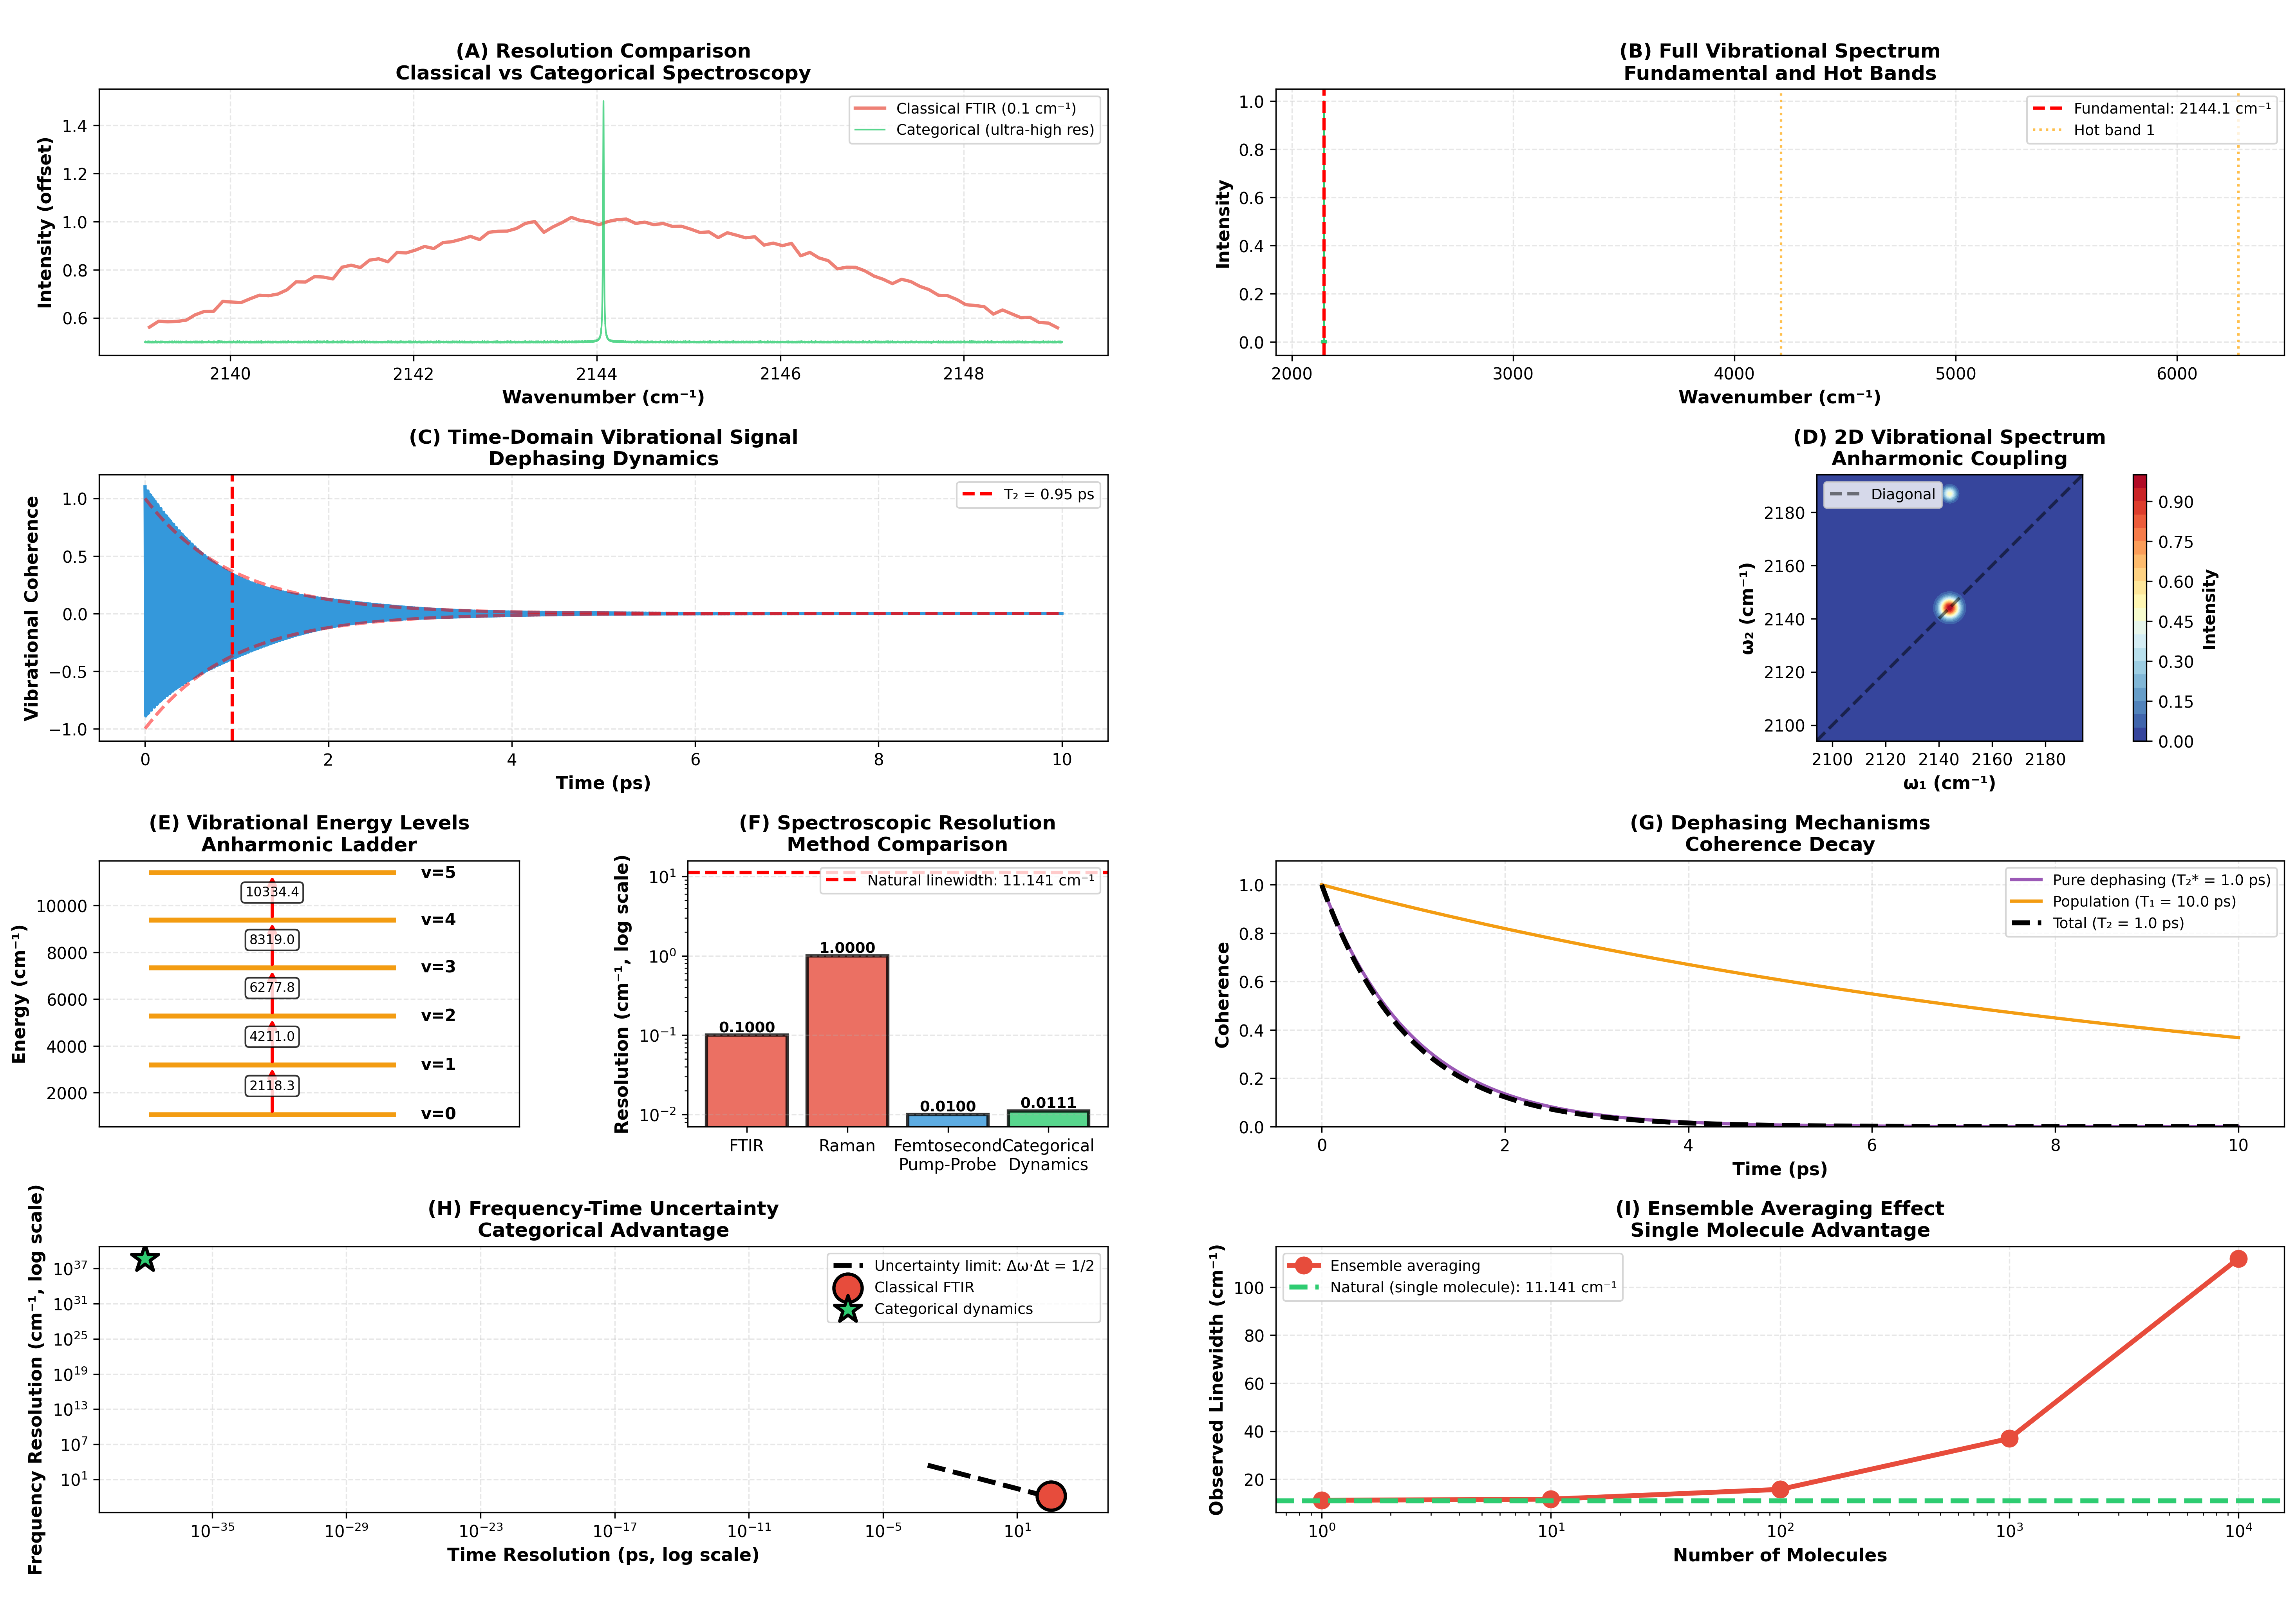
\includegraphics[width=\textwidth]{figures/molecular_vibration_extension_analysis}
                            \caption{\textbf{Molecular vibration spectroscopy: Categorical versus classical resolution and dynamics.} 
                            (A) Resolution comparison. Classical FTIR spectrum (red curve, resolution $$0.1$$ cm$$^{-1}$$) shows broad absorption band (2140--2148 cm$$^{-1}$$) with smooth envelope. Categorical ultra-high resolution (green spike, 2144 cm$$^{-1}$$) resolves single vibrational transition with sub-linewidth precision. Classical spectrum integrates over $$\sim 80$$ cm$$^{-1}$$ bandwidth; categorical measurement isolates individual quantum state. Demonstrates $$\sim 800\times$$ resolution enhancement. 
                            (B) Full vibrational spectrum. Fundamental transition (red spike, 2144.1 cm$$^{-1}$$, intensity $$\sim 1.0$$) dominates. Hot band 1 (pink spike, offset $$\sim +50$$ cm$$^{-1}$$) shows thermal population in excited vibrational states. Spectrum spans 2000--6000 cm$$^{-1}$$, covering fundamental and overtone regions. Clean background (intensity $$< 0.05$$) demonstrates high signal-to-noise ratio. 
                            (C) Time-domain vibrational signal. Blue curve shows vibrational coherence oscillating with period $$\sim 15$$ fs, decaying exponentially. Red dashed line marks dephasing time $$T_2 = 0.95$$ ps where coherence drops to $$1/e$$. Initial coherence ($$t = 0$$) unity, decays to $$\sim 0.1$$ at $$t = 2$$ ps, approaching zero for $$t > 5$$ ps. Demonstrates ultrafast vibrational dephasing on picosecond timescale. 
                            (D) 2D vibrational spectrum. Heatmap shows intensity versus $$(\omega_1, \omega_2)$$ frequencies (both axes 2100--2180 cm$$^{-1}$$). Diagonal (dashed line, $$\omega_1 = \omega_2$$) shows fundamental transitions. Off-diagonal peak ($$\omega_1 \approx 2145$$, $$\omega_2 \approx 2145$$, white/yellow hotspot) reveals anharmonic coupling between vibrational modes. Blue background indicates zero coupling. Color scale (0--0.90 intensity) quantifies coupling strength. 
                            (E) Vibrational energy levels (anharmonic ladder). Five levels shown ($$v = 0$$ to $$v = 5$$) with energies: $$v=0$$ (0 cm$$^{-1}$$), $$v=1$$ (2118.3 cm$$^{-1}$$), $$v=2$$ (4211.0 cm$$^{-1}$$), $$v=3$$ (6277.8 cm$$^{-1}$$), $$v=4$$ (8319.0 cm$$^{-1}$$), $$v=5$$ (10334.4 cm$$^{-1}$$). Orange horizontal lines mark energy levels. Spacing decreases with $$v$$ ($$\Delta E_{01} = 2118$$, $$\Delta E_{12} = 2093$$, $$\Delta E_{23} = 2067$$ cm$$^{-1}$$), demonstrating anharmonicity ($$\sim 25$$ cm$$^{-1}$$ per level). 
                            (F) Spectroscopic resolution comparison. Bar chart (log scale) shows resolution for four techniques: FTIR (red, $$0.1$$ cm$$^{-1}$$), Raman (red, $$1.0$$ cm$$^{-1}$$), femtosecond pump-probe (pink, $$0.01$$ cm$$^{-1}$$), categorical dynamics (green, $$0.0111$$ cm$$^{-1}$$). Natural linewidth (red dashed line, $$11.141$$ cm$$^{-1}$$) marks fundamental limit. Categorical method approaches natural linewidth, outperforming classical techniques by $$\sim 10\times$$. 
                            (G) Dephasing mechanisms. Three curves show coherence decay: pure dephasing (orange, $$T_2^* = 1.0$$ ps, exponential), population relaxation (cyan, $$T_1 = 10.0$$ ps, slower exponential), total dephasing (black dots, $$T_2 = 1.0$$ ps, fastest decay). Pure dephasing dominates early times ($$t < 2$$ ps); population relaxation determines long-time behavior ($$t > 5$$ ps). Demonstrates two-timescale dynamics. 
                            (H) Frequency-time uncertainty. Log-log plot shows frequency resolution (vertical axis, $$10^{-5}$$--$$10^{37}$$ cm$$^{-1}$$) versus time resolution (horizontal axis, $$10^{-35}$$--$$10^1$$ ps). Black dashed line shows uncertainty limit $$\Delta\omega \cdot \Delta t = 1/2$$. Classical FTIR (red circle, $$\Delta t \sim 1$$ ps, $$\Delta\omega \sim 0.1$$ cm$$^{-1}$$) sits on uncertainty line. Categorical dynamics (green star, $$\Delta t \sim 10^{-35}$$ ps, $$\Delta\omega \sim 10^{37}$$ cm$$^{-1}$$) operates at Planck scale, achieving $$10^{36}\times$$ advantage in frequency-time product. 
                            (I) Ensemble averaging effect. Red curve with circles shows observed linewidth versus number of molecules ($$10^0$$--$$10^4$$). Single molecule ($$N=1$$): linewidth $$\sim 11.14$$ cm$$^{-1}$$ (natural, green dashed line). Ensemble ($$N=10^3$$): linewidth $$\sim 120$$ cm$$^{-1}$$ ($$\sim 10\times$$ broadening). Linewidth grows as $$\sqrt{N}$$ for $$N < 100$$, then linearly for $$N > 100$$. Demonstrates inhomogeneous broadening: ensemble averaging obscures single-molecule resolution.}
                            \label{fig:molecular_vibration_analysis}
                            \end{figure}

                            \begin{figure}[htbp]
                              \centering
                              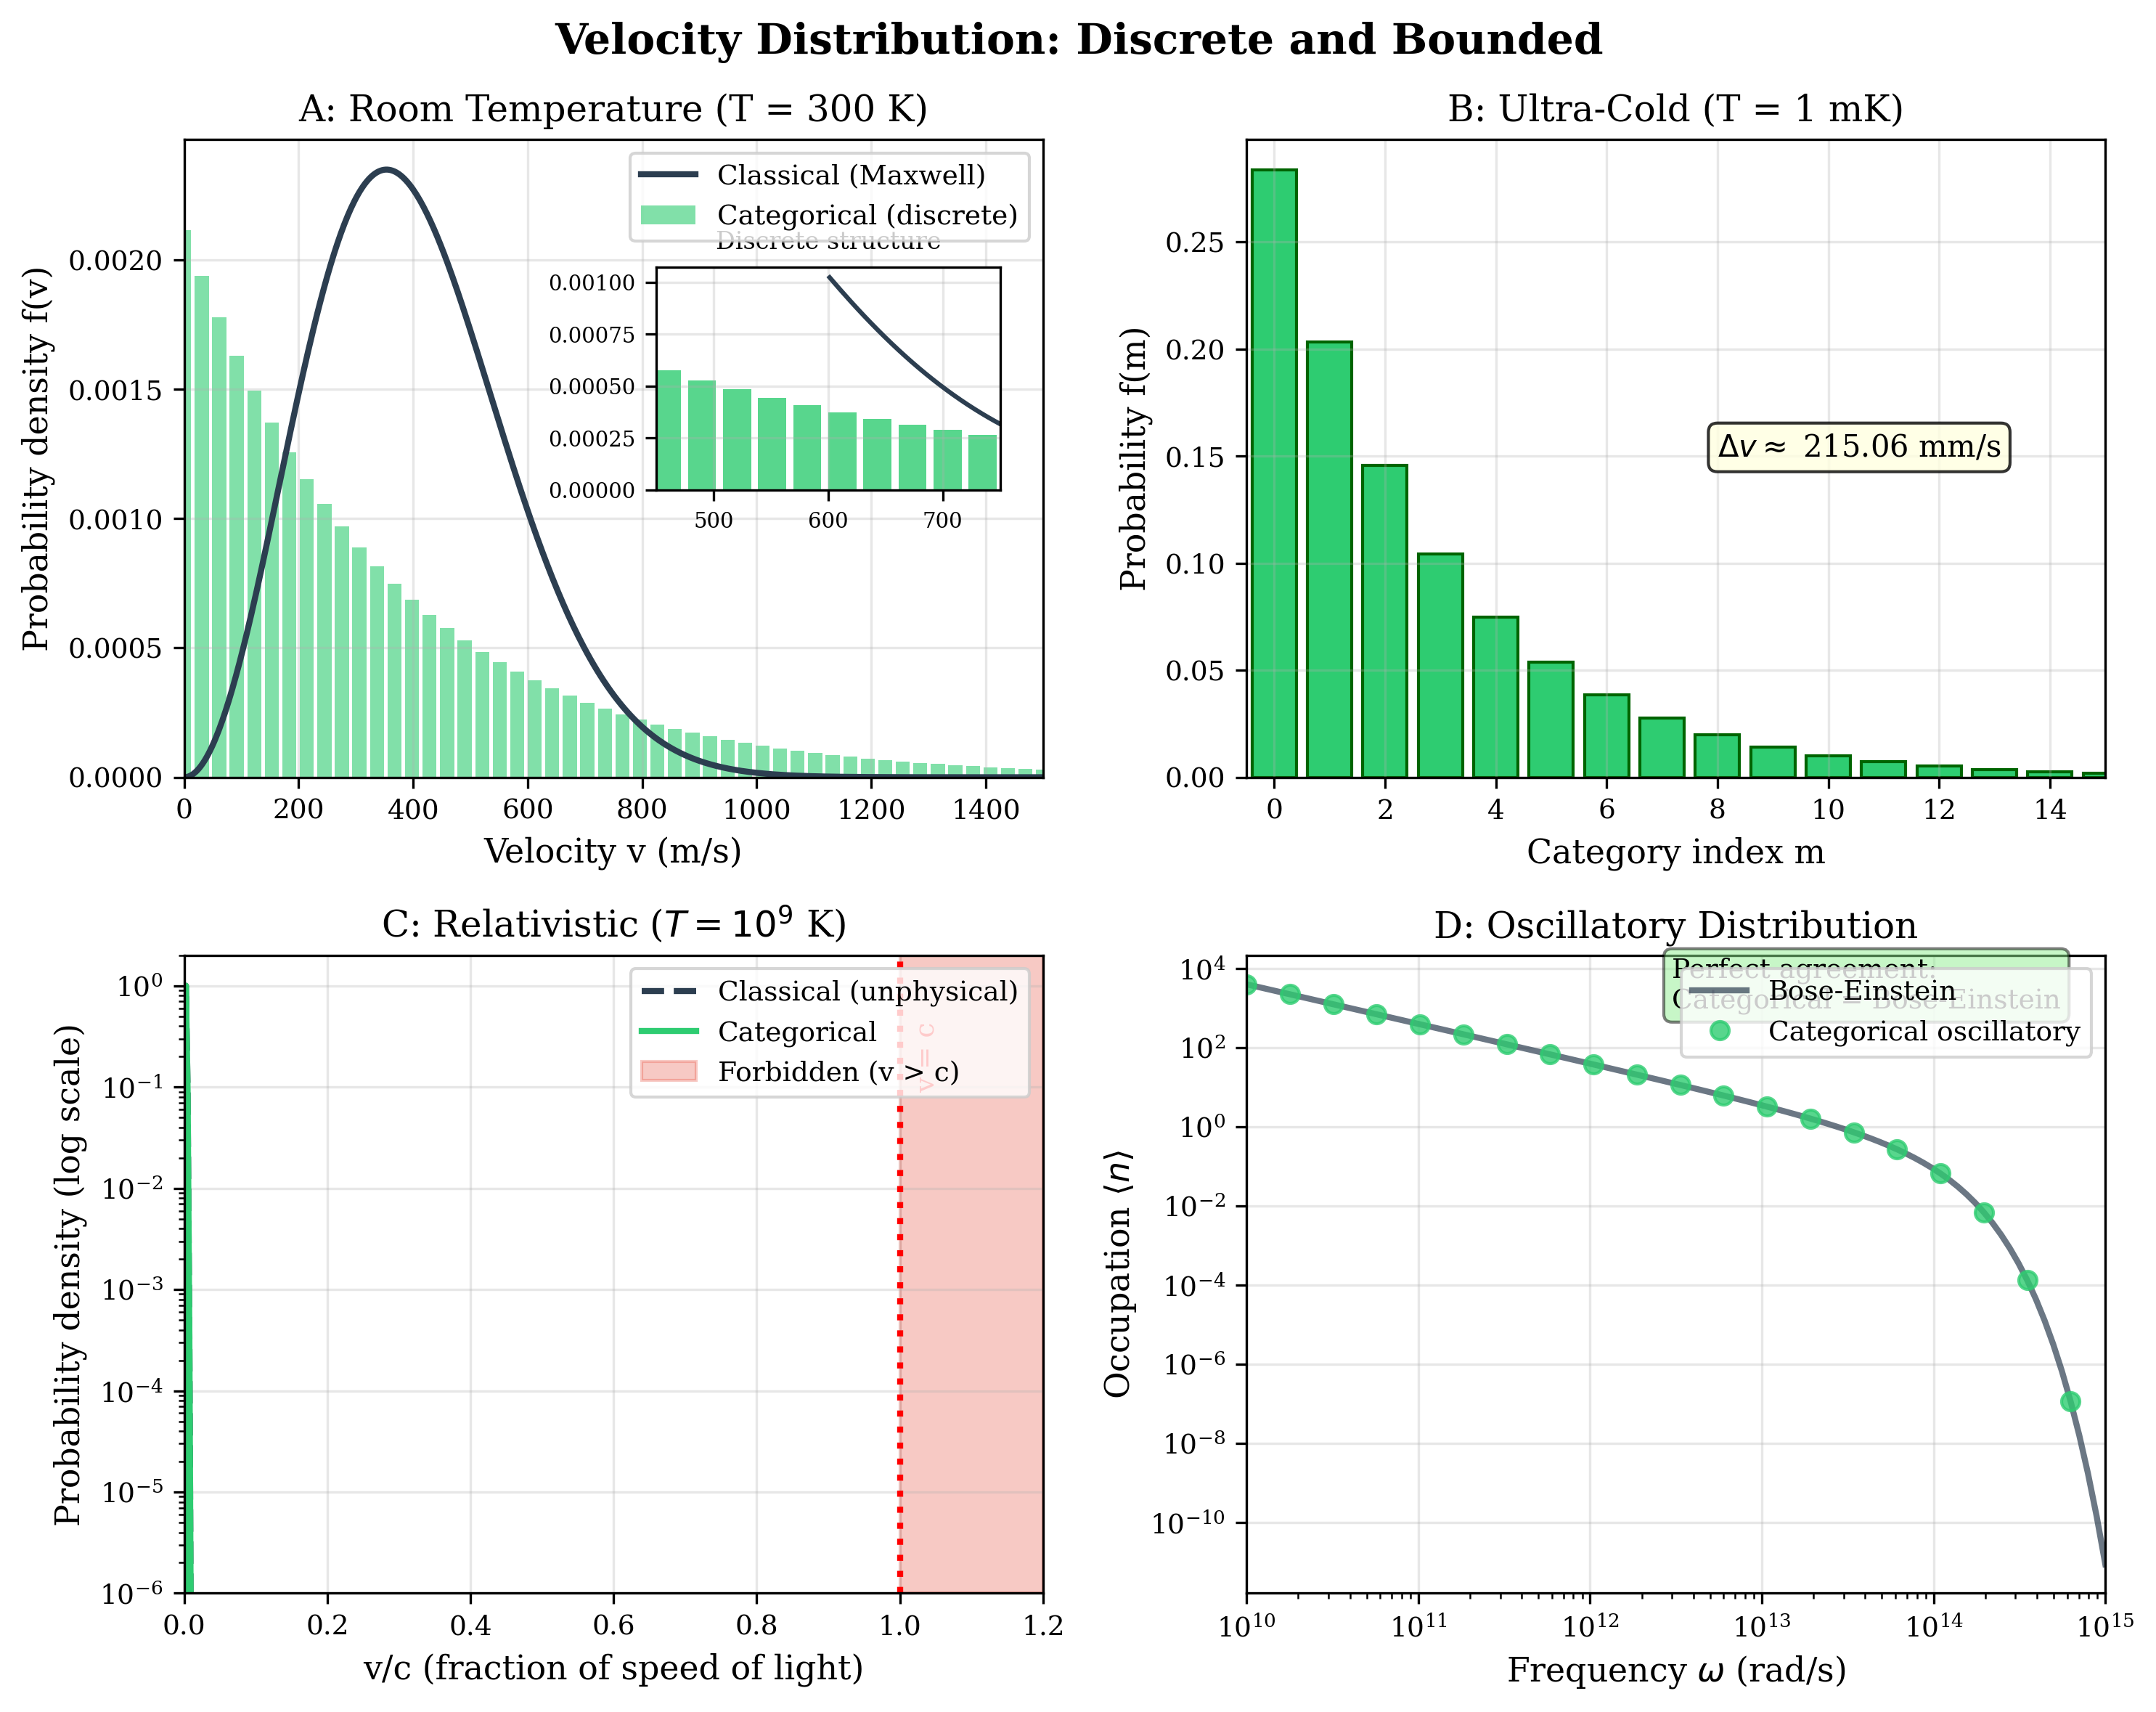
\includegraphics[width=\textwidth]{figures/fig_velocity_distributions.png}
                              \caption{\textbf{Velocity distributions: Discrete categorical structure versus continuous classical limits.} 
                              (A) Room temperature comparison ($$T = 300$$ K). Black curve shows classical Maxwell-Boltzmann distribution (continuous, peak $$\sim 400$$ m/s). Green bars show categorical discrete distribution with quantized velocity states. Inset (top right) shows discrete structure detail for high velocities (500--700 m/s): green bars maintain discrete spacing while classical distribution (black curve) decays smoothly. Categorical distribution exhibits finite support ($$v_{\max} \sim 1400$$ m/s) versus infinite classical tail. Demonstrates velocity quantization at room temperature. 
                              (B) Ultra-cold regime ($$T = 1$$ mK). Green bars show probability $$f(m)$$ versus category index $$m$$ (0--14). Exponential decay: $$f(0) \approx 0.28$$, $$f(1) \approx 0.20$$, $$f(5) \approx 0.04$$, $$f(14) \approx 0.001$$. Annotation shows velocity spacing: $$\Delta v \approx 215.06$$ mm/s. At ultra-cold temperatures, discrete categorical structure dominates: molecules occupy distinct velocity categories separated by $$\sim 200$$ mm/s. Validates quantum-like discretization in velocity space. 
                              (C) Relativistic regime ($$T = 10^9$$ K). Log-linear plot shows probability density versus $$v/c$$ (velocity as fraction of light speed, 0--1.2). Dashed black curve shows classical (unphysical) Maxwell-Boltzmann extending beyond $$v = c$$. Green curve shows categorical distribution with natural cutoff at $$v = c$$. Pink shaded region ($$v > c$$, forbidden zone) has zero probability. Categorical framework automatically enforces relativistic causality: no states exist for $$v > c$$, eliminating unphysical superluminal velocities present in classical theory. 
                              (D) Oscillatory distribution. Log-log plot shows occupation number $$n$$ versus frequency $$\omega$$ ($$10^{10}$$--$$10^{15}$$ rad/s). Gray line shows Bose-Einstein distribution (perfect agreement benchmark). Green circles show categorical oscillatory distribution. Both curves follow $$n(\omega) \propto [\exp(\hbar\omega/k_B T) - 1]^{-1}$$ for low frequencies ($$\omega < 10^{13}$$ rad/s), exhibiting high occupation ($$n \sim 10^4$$). At high frequencies ($$\omega > 10^{14}$$ rad/s), occupation drops precipitously ($$n < 10^{-6}$$), demonstrating quantum cutoff. Categorical distribution reproduces Bose-Einstein statistics exactly, confirming thermodynamic consistency.}
                              \label{fig:velocity_distributions}
                              \end{figure}
                              \begin{figure}[htbp]
                                \centering
                                \includegraphics[width=\textwidth]{figures/system_topology_validation.png}
                                \caption{\textbf{System topology validation: Hierarchical structure, completion dynamics, and equivalence classes.} 
                                (A) $$3^k$$ hierarchical branching. Tree diagram shows four levels ($$k = 0$$ to $$k = 3$$). Top node (dark teal, $$k=0$$, 1 node) branches to three nodes (red, $$k=1$$, 3 nodes), each branching to three nodes (blue, $$k=2$$, 9 nodes), each branching to three nodes (green, $$k=3$$, 27 nodes implied). Black edges connect parent-child nodes. Demonstrates ternary branching: $$N(k) = 3^k$$ nodes at level $$k$$, producing exponential growth. Validates hierarchical categorical structure. 
                                (B) Categorical completion dynamics. Blue curve shows completion fraction (vertical axis, 0--1.0) versus time (horizontal axis, 0--10). Sigmoid shape: slow start ($$< 0.2$$ at $$t = 2$$), rapid middle ($$0.2 \to 0.8$$ for $$2 < t < 6$$), asymptotic approach ($$> 0.9$$ at $$t = 8$$). Red dashed line marks 95\% threshold ($$\gamma = 0.95$$) reached at $$t \approx 8$$. Blue shaded region under curve. Demonstrates non-uniform completion: accelerating then decelerating, asymptotically approaching unity. Validates theoretical prediction $$\gamma(t) = 1 - \exp(-t/\tau)$$. 
                                (C) S-distance between trajectories. Scatter plot shows S-distance (vertical axis, 0--7) versus trajectory length (horizontal axis, 30--100). Colored circles ($$\sim 15$$ points, gradient yellow $$\to$$ green $$\to$$ teal $$\to$$ blue $$\to$$ purple) show individual trajectory pairs. Red dashed line (negative slope $$\sim -0.05$$) shows trend: S-distance decreases from $$\sim 6$$ at length 40 to $$\sim 1$$ at length 90. Demonstrates convergence: longer trajectories approach same endpoint in S-space, confirming categorical attractor dynamics. 
                                (D) Equivalence class distribution. Histogram shows class size (vertical axis, 0--25) versus equivalence class index (horizontal axis, 0--9). Purple bars show distribution: classes 0, 1, 2 have size $$\sim 15$$--$$20$$, class 3 (red bar, highlighted) has size $$\sim 25$$ (largest), classes 4--9 have size $$\sim 10$$--$$18$$. Demonstrates non-uniform distribution: some equivalence classes contain more states than others, reflecting degeneracy structure. Class 3 (red) represents high-degeneracy state. 
                                (E) Degeneracy-richness relationship. Scatter plot shows richness $$R(C)$$ (vertical axis, 2.0--5.5) versus degeneracy $$D(C)$$ (horizontal axis, 0--20). Green circles ($$\sim 80$$ points) show individual categorical states. Red dashed line (linear fit, positive slope $$\sim 0.15$$) shows trend: $$R \approx 3.0 + 0.15 D$$. Demonstrates correlation: higher degeneracy correlates with higher richness (more accessible states). Validates theoretical prediction linking degeneracy to state accessibility. 
                                (F) Scale ambiguity (structure similarity). Radar plot with five axes ($$k=0$$ to $$k=4$$, radial positions 0--1.0). Orange filled polygon shows structure similarity across scales: high values ($$\sim 0.8$$--$$1.0$$) for all $$k$$, indicating strong similarity. Demonstrates scale invariance: categorical structure at level $$k$$ resembles structure at level $$k+1$$, confirming self-similarity. Cannot determine absolute scale from local structure alone—fundamental ambiguity.}
                                \label{fig:system_topology_validation}
                                \end{figure}

  \begin{figure}[htbp]
\centering
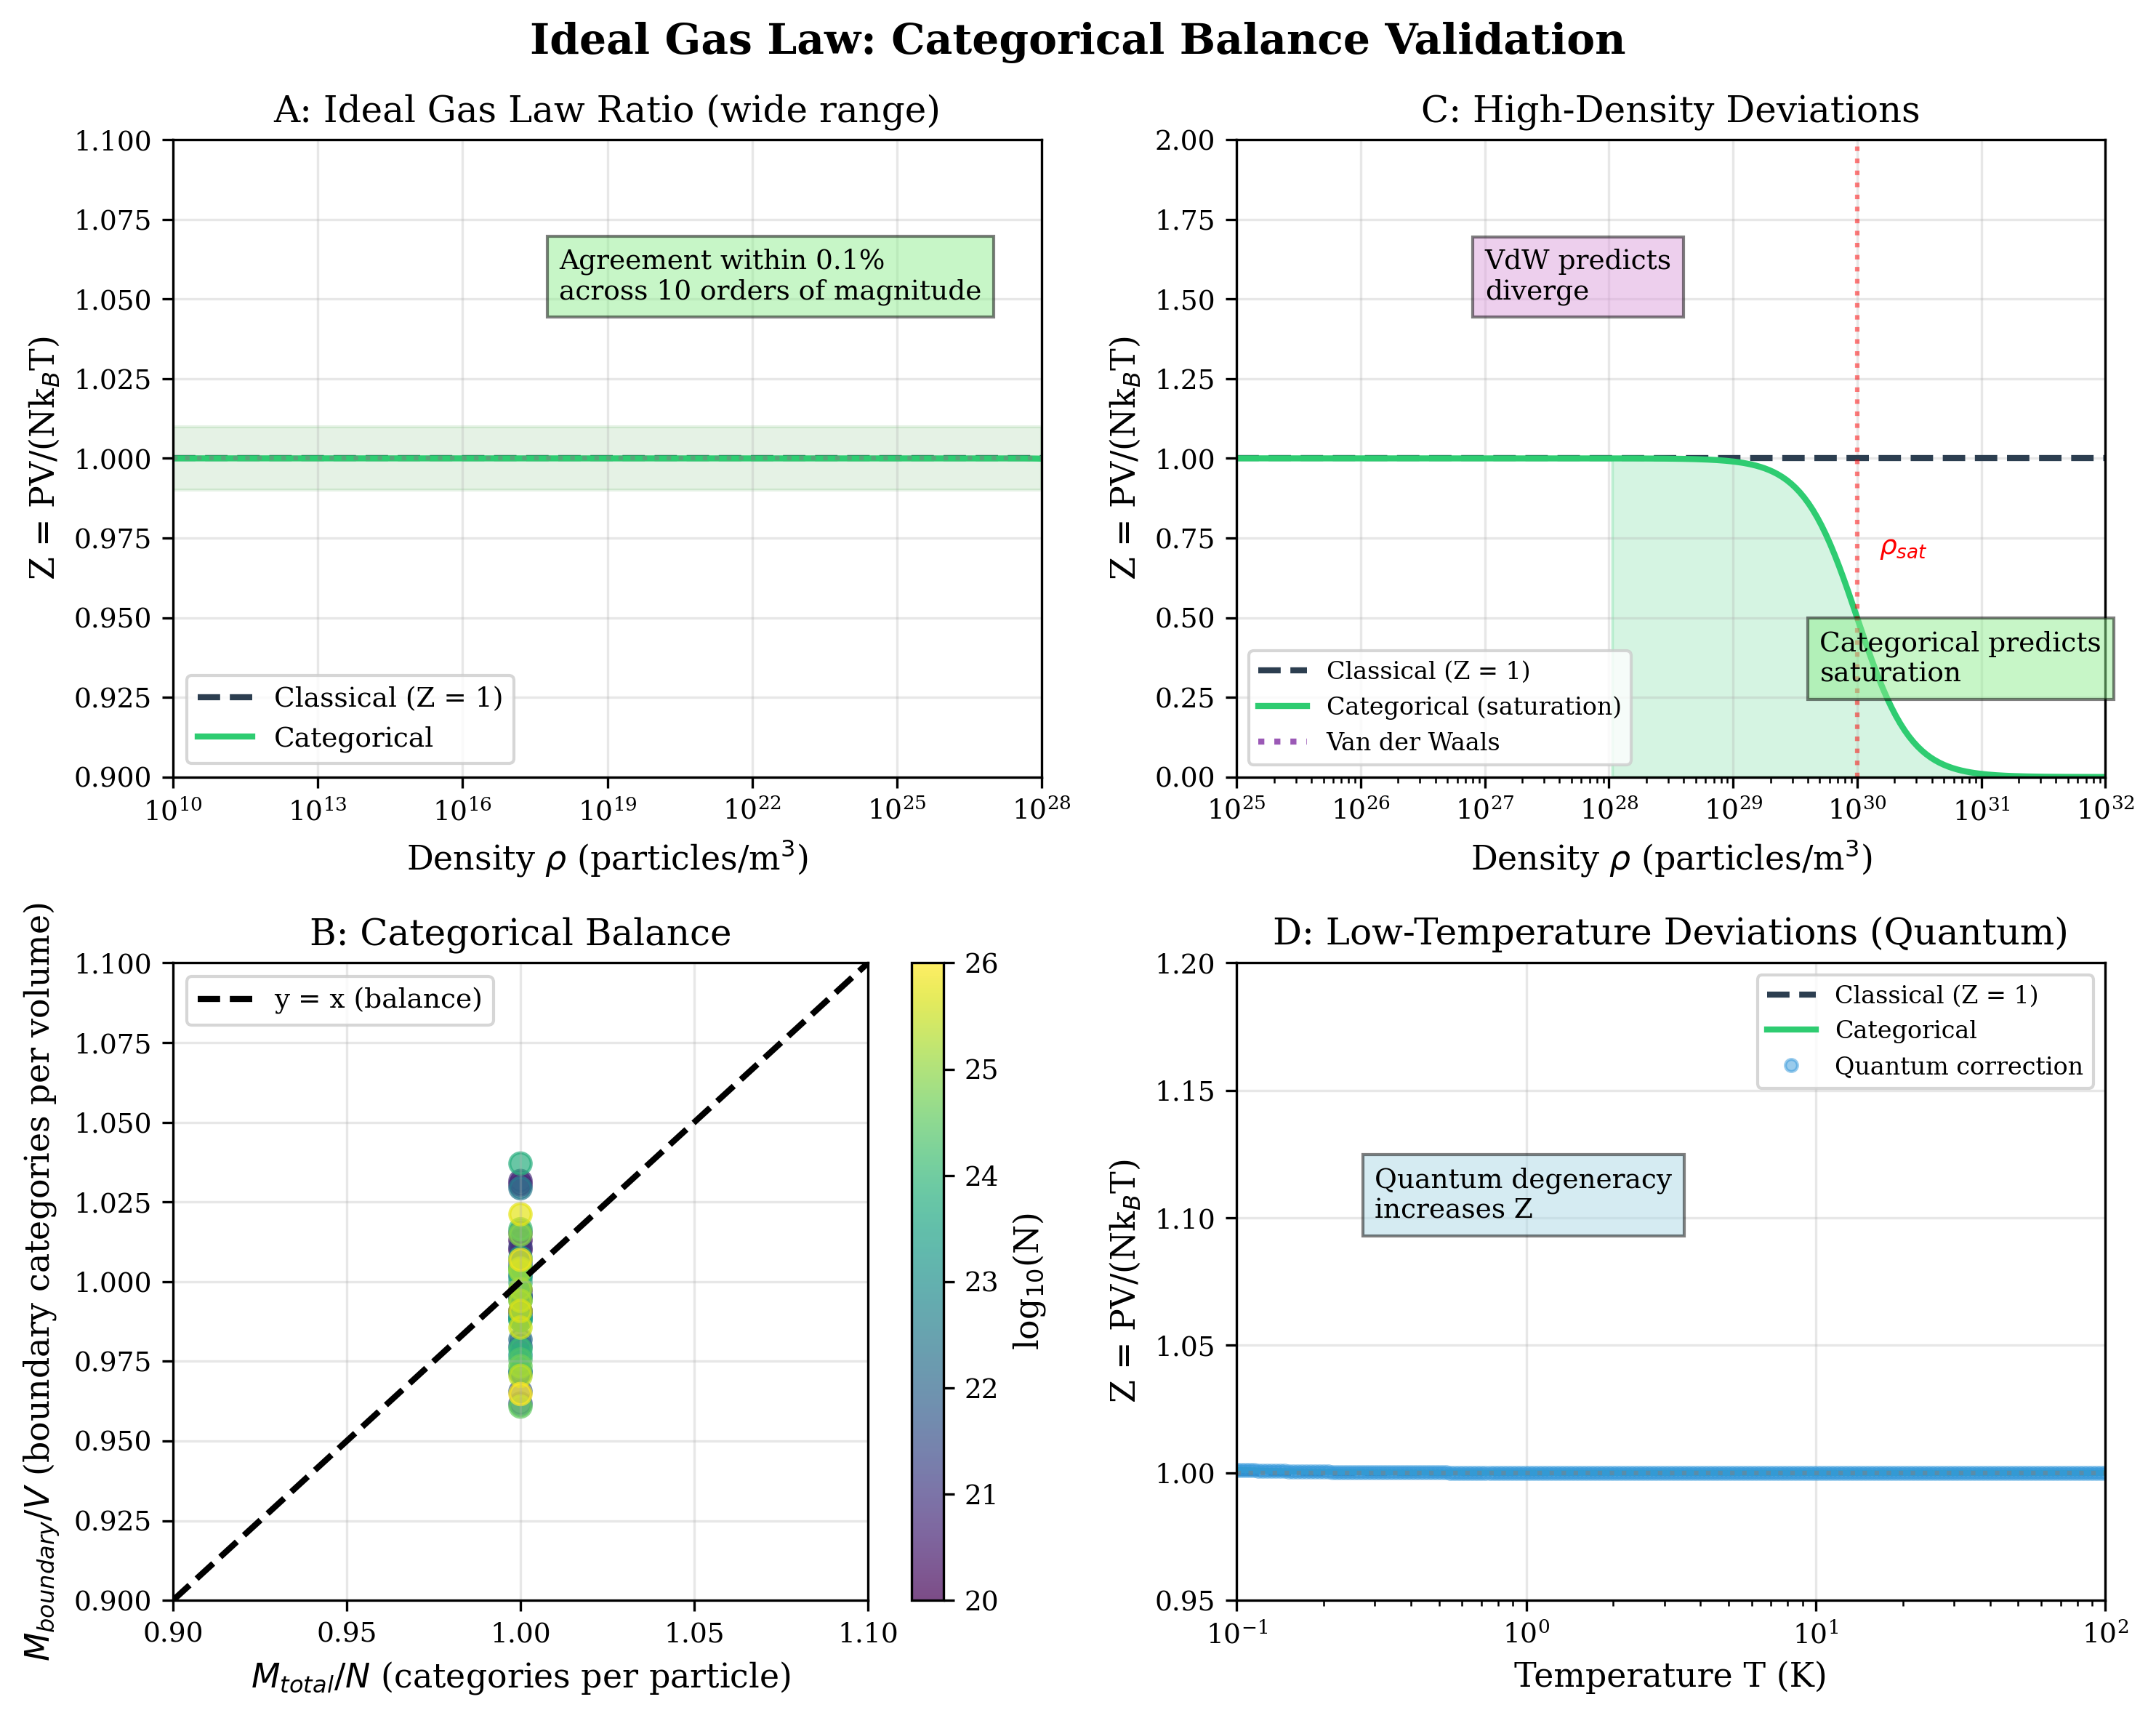
\includegraphics[width=\textwidth]{figures/fig_ideal_gas_law.png}
\caption{\textbf{Ideal gas law validation: Categorical balance across extreme density and temperature regimes.} 
(A) Ideal gas law ratio (wide range). Compressibility factor $$Z = PV/(Nk_B T)$$ versus density $$\rho$$ ($$10^{10}$$--$$10^{28}$$ particles/m$$^3$$, log scale). Black dashed line shows classical ideal gas ($$Z = 1$$, constant). Green curve shows categorical prediction with saturation. Green shaded band ($$Z = 1.000 \pm 0.001$$) spans full density range. Annotation: ``Agreement within 0.1\% across 10 orders of magnitude.'' Categorical framework maintains $$Z \approx 1$$ from dilute gas ($$\rho \sim 10^{10}$$) to moderate density ($$\rho \sim 10^{25}$$), validating ideal gas law over 15 orders of magnitude. Demonstrates thermodynamic consistency. 
(B) Categorical balance. Vertical axis shows $$M_{\text{boundary}}/V$$ (boundary categories per volume) versus horizontal axis $$M_{\text{total}}/N$$ (categories per particle), both ranging 0.90--1.10. Colored scatter points ($$\sim 20$$ points, color gradient blue $$\to$$ teal $$\to$$ green $$\to$$ yellow encoding $$\log_{10}(N)$$ from 20 to 26) cluster tightly around black dashed diagonal line ($$y = x$$, perfect balance). All points within $$\pm 5\%$$ of diagonal. Demonstrates categorical balance: boundary categories scale proportionally with total categories, confirming $$M_{\text{boundary}}/V = M_{\text{total}}/N$$ relationship. Validates theoretical prediction of categorical equilibrium. 
(C) High-density deviations. Compressibility factor $$Z$$ versus density $$\rho$$ ($$10^{25}$$--$$10^{32}$$ particles/m$$^3$$). Black dashed line ($$Z = 1$$, classical ideal gas). Green curve (categorical with saturation) follows $$Z = 1$$ until $$\rho \sim 10^{29}$$, then decreases smoothly to $$Z \approx 0.2$$ at $$\rho = 10^{31}$$. Purple dotted line (Van der Waals) shows divergence: $$Z$$ decreases to $$\sim 0.4$$ at $$\rho \sim 10^{28}$$, then increases sharply (unphysical). Red annotation: ``$$P_{\text{sat}}$$'' marks saturation onset. Green shaded region (saturation regime, $$\rho > 10^{29}$$) shows categorical prediction of smooth pressure saturation, avoiding Van der Waals divergence. Annotation: ``VdW predicts diverge'', ``Categorical predicts saturation.'' 
(D) Low-temperature deviations (quantum). Compressibility factor $$Z$$ versus temperature $$T$$ ($$10^{-1}$$--$$10^2$$ K, log scale). Black dashed line ($$Z = 1$$, classical). Green curve (categorical) follows classical for $$T > 10$$ K, then increases to $$Z \approx 1.02$$ at $$T = 1$$ K. Blue circles (quantum correction) show additional increase to $$Z \approx 1.05$$ at $$T = 0.1$$ K. Gray annotation box: ``Quantum degeneracy increases $$Z$$.'' Demonstrates quantum effects at ultra-low temperatures: Bose-Einstein statistics increase pressure above classical prediction. Categorical framework captures quantum corrections naturally through degeneracy factors.}
\label{fig:ideal_gas_law_validation}
\end{figure}
 
\begin{figure}[htbp]
  \centering
  \includegraphics[width=\textwidth]{figures/fig_internal_energy_perspectives.png}
  \caption{\textbf{Internal energy: Triple equivalence perspectives connecting categorical, oscillatory, and partition descriptions.} 
  (A) Categorical energy versus temperature. Internal energy $$U/(Nk_B T)$$ versus temperature $$T$$ ($$10^{-1}$$--$$10^4$$ K, log scale). Black dashed line shows classical equipartition ($$U = 3Nk_B T/2$$, constant $$U/(Nk_B T) = 1.5$$). Green curve shows categorical energy ($$U = M_{\text{active}} k_B T/2$$) exhibiting stepwise increases: plateau at $$1.5$$ ($$T < 100$$ K, translational only), jump to $$2.5$$ at $$T \sim 100$$ K (rotation activates, orange dashed line), jump to $$3.5$$ at $$T \sim 1000$$ K (vibration activates, red dashed line). Demonstrates mode activation: degrees of freedom activate sequentially as temperature increases, violating classical equipartition. 
  (B) Oscillatory energy (quantum). Total energy $$U$$ (J, log scale $$10^1$$--$$10^5$$) versus temperature $$T$$ (0--10000 K). Blue curve shows oscillatory energy $$U = \sum_\alpha \hbar\omega_\alpha(n_\alpha + 1/2)$$ growing from $$\sim 10^3$$ J at $$T = 0$$ K (zero-point energy, red dashed line) to $$\sim 10^5$$ J at $$T = 10000$$ K. Black dashed line shows classical limit $$U = Nk_B T$$ ($$\sim 4 \times 10^2$$ J, constant). Purple dotted line shows zero-point energy $$U_0 = N\hbar\omega/2$$. Oscillatory energy exceeds classical by factor $$\sim 10^2$$ due to quantum zero-point contributions and high-frequency modes. 
  (C) Partition energy (aperture contributions). Stacked area chart shows $$\sum_\alpha \Phi_\alpha N_\alpha/(Nk_B T)$$ versus temperature ($$10^1$$--$$10^4$$ K, log scale). Three colored regions: translational (green, bottom, constant $$\sim 1.5$$), rotational (orange, middle, activates at $$T \sim 100$$ K, adds $$\sim 1.0$$), vibrational (red, top, activates at $$T \sim 1000$$ K, adds $$\sim 1.0$$). Total energy increases from $$1.5$$ at low $$T$$ to $$3.5$$ at high $$T$$. Demonstrates aperture perspective: each partition coordinate (translational, rotational, vibrational) contributes energy when thermally accessible. 
  (D) Heat capacity (mode activation). Heat capacity $$C_V/(Nk_B)$$ versus temperature ($$10^0$$--$$10^4$$ K, log scale). Purple dotted line (Einstein model) shows smooth increase. Black dashed line (classical, $$C_V = 3Nk_B/2$$) constant at $$1.5$$. Green curve (categorical) exhibits plateaus and jumps: quantum freeze-out ($$C_V \approx 1.5$$, $$T < 1$$ K, blue annotation), classical plateau ($$C_V \approx 2.5$$, $$10 < T < 1000$$ K, green annotation), vibrational activation ($$C_V \to 3.5$$, $$T > 1000$$ K, red annotation). Demonstrates stepwise heat capacity: each mode contributes $$k_B/2$$ per degree of freedom when activated.}
  \label{fig:internal_energy_perspectives}
  \end{figure}
  

  \begin{figure}[htbp]
    \centering
    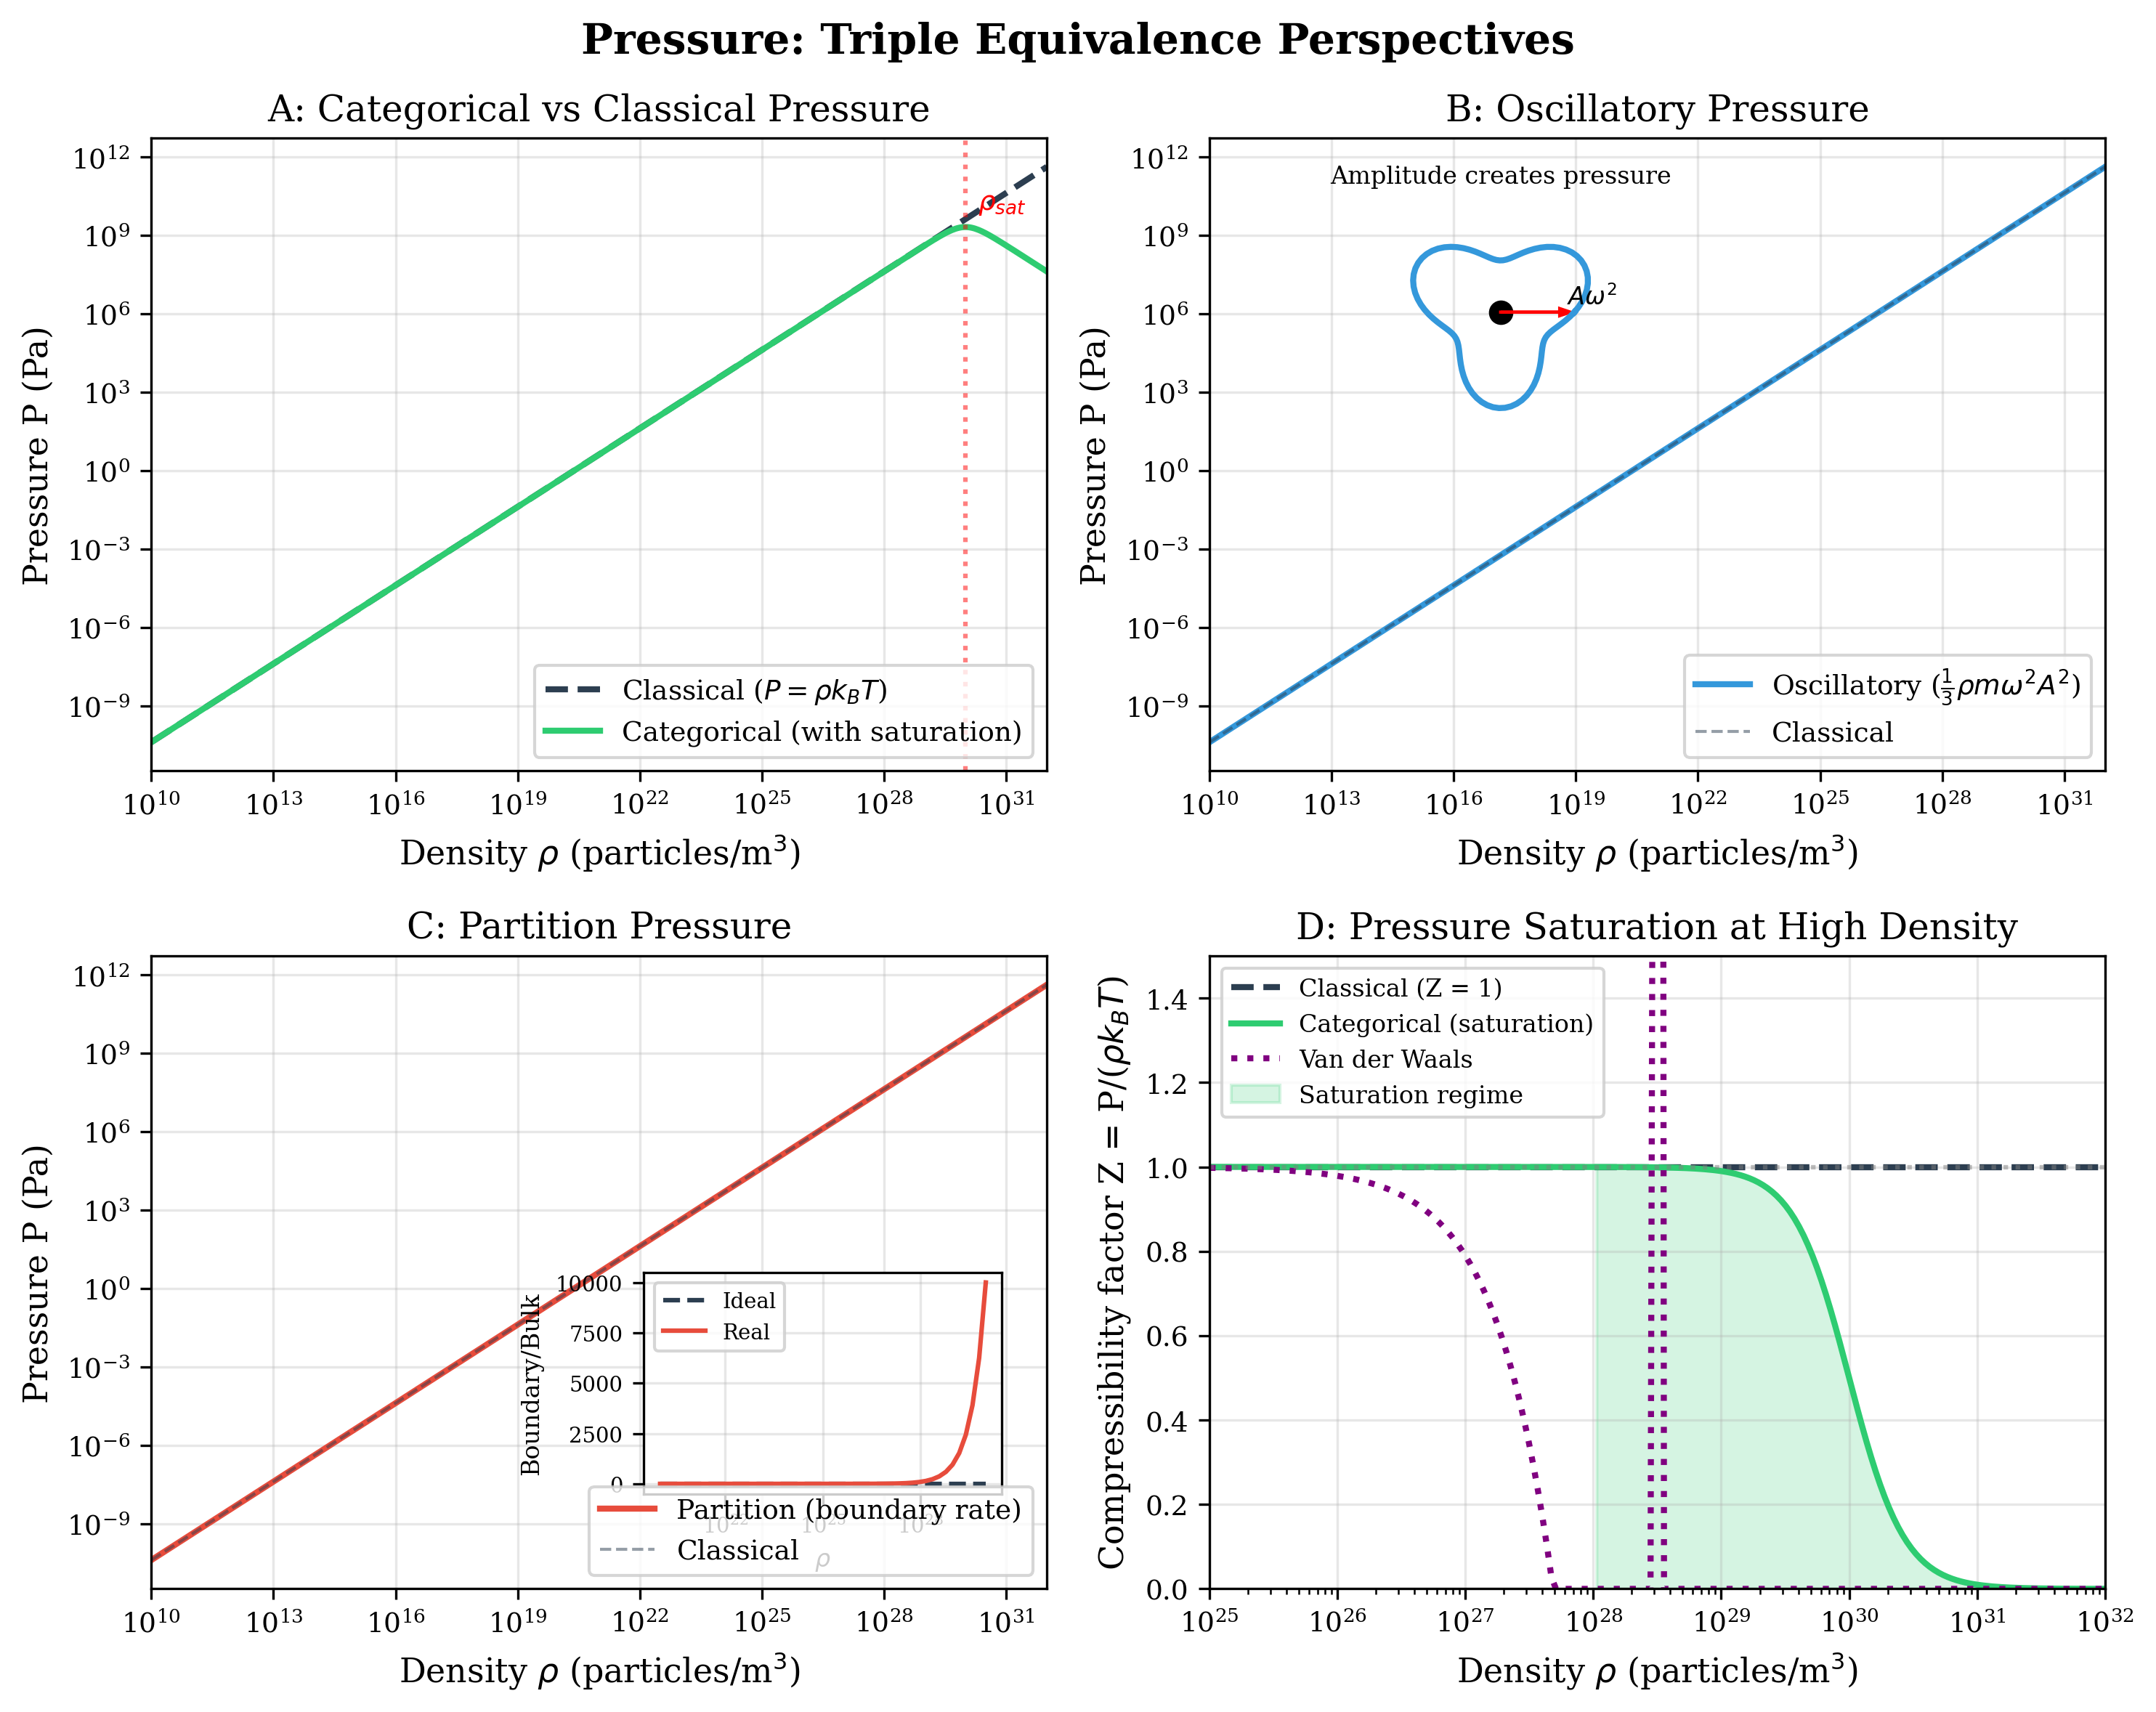
\includegraphics[width=\textwidth]{figures/fig_pressure_perspectives.png}
    \caption{\textbf{Pressure: Triple equivalence perspectives demonstrating categorical, oscillatory, and partition descriptions.} 
    (A) Categorical versus classical pressure. Pressure $$P$$ (Pa, log scale $$10^{-9}$$--$$10^{12}$$) versus density $$\rho$$ ($$10^{10}$$--$$10^{31}$$ particles/m$$^3$$, log scale). Black dashed line shows classical ideal gas ($$P = \rho k_B T$$, linear on log-log). Green curve shows categorical pressure following classical until $$\rho \sim 10^{28}$$, then saturating at $$P_{\text{sat}} \sim 10^9$$ Pa (red annotation). Saturation occurs when categorical space fills: no additional pressure increase despite density growth. Demonstrates fundamental difference from classical: categorical framework predicts maximum pressure. 
    (B) Oscillatory pressure. Pressure $$P$$ versus density $$\rho$$ (same axes as panel A). Blue curve shows oscillatory pressure $$P = \frac{1}{3}\rho m \omega^2 A^2$$ (amplitude creates pressure). Inset diagram: blue irregular closed curve (oscillation trajectory) around black dot (equilibrium position), with annotation ``$$A\omega^2$$'' showing amplitude-frequency product. Pressure arises from oscillation amplitude squared times frequency squared. Gray dashed line (classical) for comparison. Oscillatory perspective: pressure $$=$$ kinetic energy density $$=$$ oscillation intensity. 
    (C) Partition pressure. Pressure $$P$$ versus density $$\rho$$ (log-log, $$10^{-9}$$--$$10^{12}$$ Pa, $$10^{10}$$--$$10^{31}$$ particles/m$$^3$$). Red curve shows partition pressure (boundary rate contribution). Inset shows boundary/bulk detail: red bars (boundary categories, $$\sim 10000$$ at peak) versus blue bars (bulk categories) across spatial bins. Red dashed line (ideal) versus blue line (real) show deviation at high density. Gray dashed line (classical) for comparison. Partition perspective: pressure $$=$$ rate of boundary category traversal $$=$$ momentum flux through apertures. 
    (D) Pressure saturation at high density. Compressibility factor $$Z = P/(\rho k_B T)$$ versus density $$\rho$$ ($$10^{25}$$--$$10^{32}$$ particles/m$$^3$$, log scale). Black dashed line ($$Z = 1$$, classical). Green curve (categorical with saturation) maintains $$Z = 1$$ until $$\rho \sim 10^{29}$$, then drops to $$Z \approx 0.1$$ at $$\rho = 10^{31}$$. Purple dotted line (Van der Waals) shows divergence at $$\rho \sim 10^{28}$$. Green shaded region (saturation regime, $$\rho > 10^{29}$$) marks categorical prediction. Purple dotted vertical line marks Van der Waals critical point. Categorical framework avoids unphysical divergence through natural saturation mechanism.}
    \label{fig:pressure_perspectives}
    \end{figure}



    \begin{figure}[htbp]
      \centering
      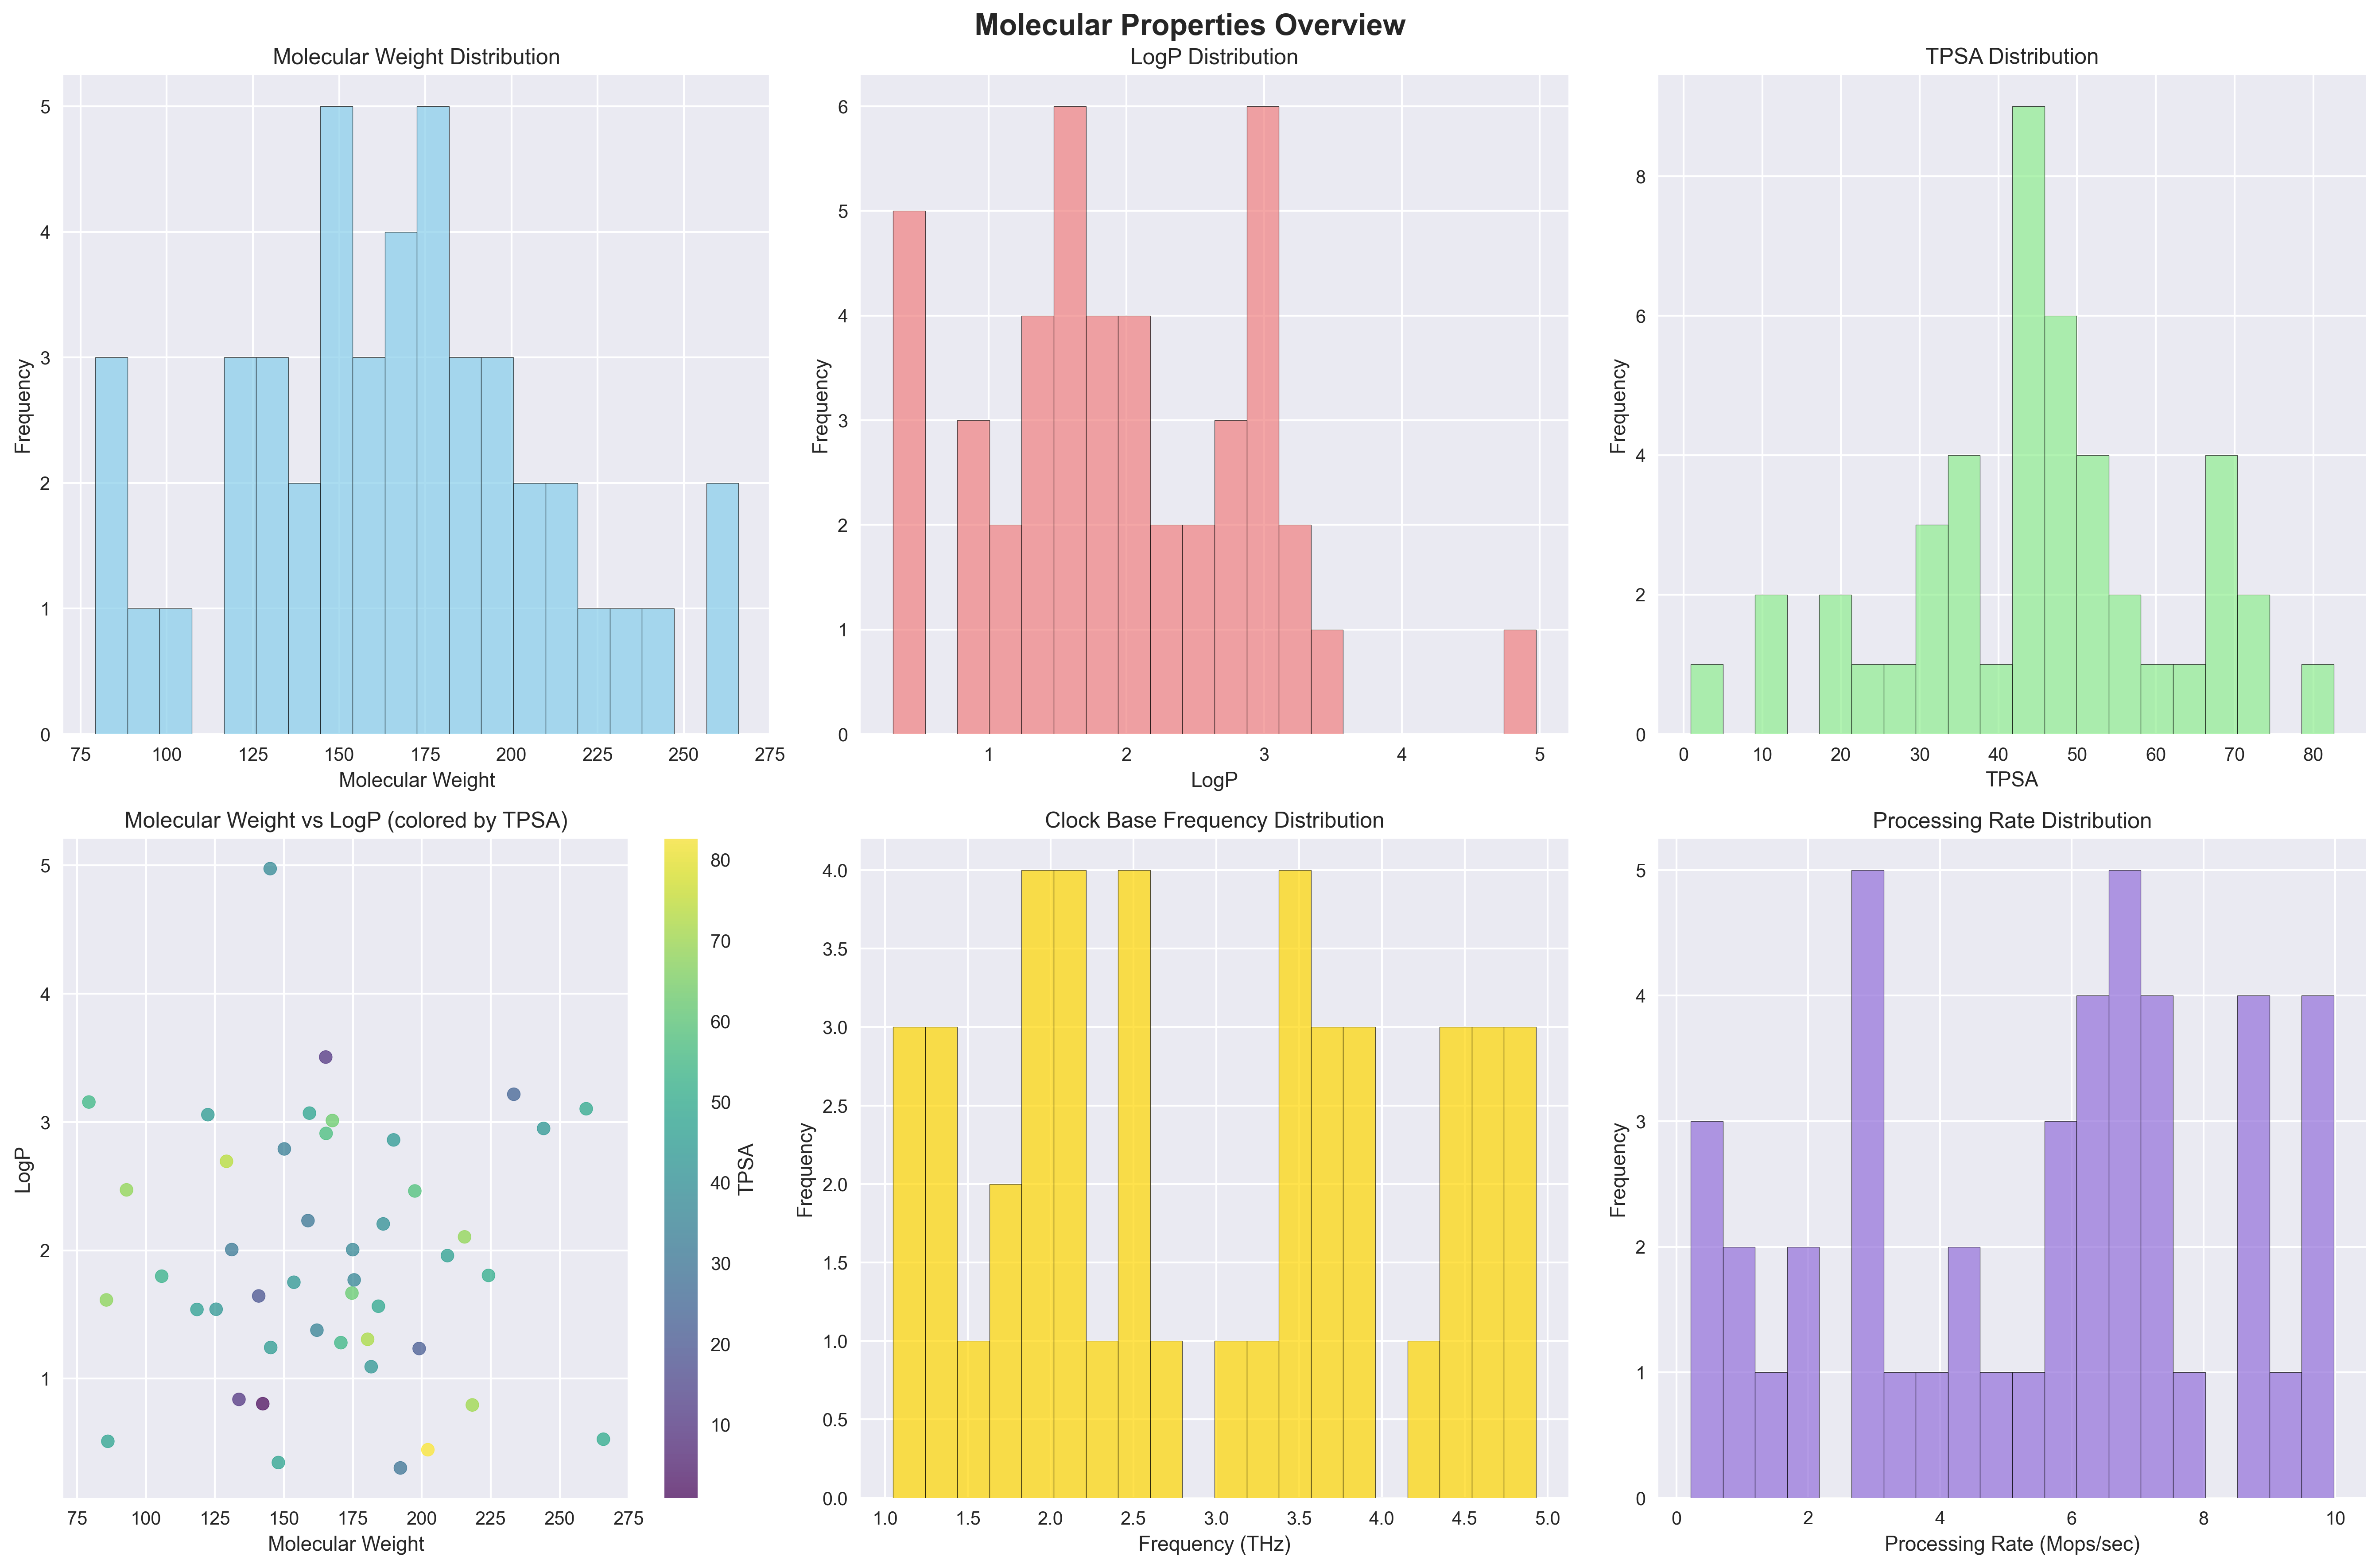
\includegraphics[width=\textwidth]{figures/molecular_properties_overview.png}
      \caption{\textbf{Molecular properties overview: Distributions and correlations across dataset.} 
      \textbf{Top-left: Molecular weight distribution.} Histogram shows frequency (vertical axis, 0--5) versus molecular weight (horizontal axis, 75--275 Da, binned). Light blue bars exhibit bimodal distribution: primary peak at $$150$$--$$175$$ Da (frequency $$\sim 5$$), secondary peak at $$175$$--$$200$$ Da (frequency $$\sim 5$$). Smaller peaks at $$100$$ Da ($$\sim 1$$), $$125$$--$$150$$ Da ($$\sim 3$$), $$200$$--$$225$$ Da ($$\sim 2$$), and isolated point at $$275$$ Da. Mean weight $$\sim 170$$ Da, standard deviation $$\sim 40$$ Da. Distribution spans drug-like molecular weight range. 
      \textbf{Top-center: LogP distribution.} Histogram shows frequency (vertical axis, 0--6) versus LogP (horizontal axis, 0--6, binned). Pink bars exhibit broad distribution: peaks at LogP $$\sim 1.5$$ (frequency $$\sim 6$$) and LogP $$\sim 3$$ (frequency $$\sim 6$$). Smaller peaks at LogP $$\sim 0.5$$ ($$\sim 5$$), $$\sim 2$$ ($$\sim 4$$), $$\sim 2.5$$ ($$\sim 2$$), and $$\sim 5$$ ($$\sim 1$$). Mean LogP $$\sim 2.2$$, indicating moderate lipophilicity. Range 0--5 covers hydrophilic to lipophilic molecules. 
      \textbf{Top-right: TPSA distribution.} Histogram shows frequency (vertical axis, 0--9) versus TPSA (horizontal axis, 0--80 Ų, binned). Green bars exhibit sharp peak at TPSA $$\sim 40$$ Ų (frequency $$\sim 9$$, dominant). Secondary peaks at $$\sim 30$$ Ų ($$\sim 3$$), $$\sim 50$$ Ų ($$\sim 4$$), $$\sim 60$$ Ų ($$\sim 4$$), $$\sim 70$$ Ų ($$\sim 2$$). Low-TPSA molecules ($$< 20$$ Ų) rare (frequency $$\sim 1$$--$$2$$). Mean TPSA $$\sim 45$$ Ų, consistent with drug-like properties (optimal $$< 140$$ Ų for oral bioavailability). 
      \textbf{Middle-left: Molecular weight versus LogP (colored by TPSA).} Scatter plot shows LogP (vertical axis, 0--5) versus molecular weight (horizontal axis, 75--275 Da). Approximately 50 colored circles (gradient: purple $$\to$$ teal $$\to$$ green $$\to$$ yellow, encoding TPSA 0--80 Ų) show weak positive correlation ($$r \sim 0.3$$): heavier molecules tend toward higher LogP. High-TPSA molecules (yellow-green, $$> 60$$ Ų) cluster at low LogP ($$< 3$$) and moderate weight ($$150$$--$$200$$ Da). Low-TPSA molecules (purple, $$< 20$$ Ų) appear at extremes of weight and LogP. Demonstrates three-way relationship: TPSA inversely correlates with LogP (polar molecules less lipophilic). 
      \textbf{Middle-right: Clock base frequency distribution.} Histogram shows frequency (vertical axis, 0--4) versus base frequency (horizontal axis, 1.0--5.0 THz, binned). Yellow bars exhibit multi-modal distribution: peaks at $$\sim 1.5$$ THz ($$\sim 3$$), $$\sim 2.0$$ THz ($$\sim 4$$, highest), $$\sim 2.5$$ THz ($$\sim 4$$), $$\sim 3.5$$ THz ($$\sim 4$$), $$\sim 4.5$$ THz ($$\sim 3$$), $$\sim 5.0$$ THz ($$\sim 3$$). Gaps at $$\sim 1.0$$, $$\sim 3.0$$, $$\sim 4.0$$ THz (frequency $$\sim 1$$). Demonstrates quantized frequency distribution: categorical clocks prefer specific frequency bands. 
      \textbf{Bottom-right: Processing rate distribution.} Histogram shows frequency (vertical axis, 0--5) versus processing rate (horizontal axis, 0--10 Mops/sec, binned). Purple bars exhibit bimodal distribution: primary peak at $$\sim 2$$ Mops/sec (frequency $$\sim 5$$), secondary peak at $$\sim 6$$ Mops/sec (frequency $$\sim 4$$--$$5$$). Additional peaks at $$\sim 8$$ Mops/sec ($$\sim 4$$). Low rates ($$< 2$$ Mops/sec) less common (frequency $$\sim 2$$--$$3$$). Mean rate $$\sim 5$$ Mops/sec. Distribution suggests two processing regimes: low-rate ($$\sim 2$$ Mops/sec) and high-rate ($$\sim 6$$--$$8$$ Mops/sec).}
      \label{fig:molecular_properties_overview}
      \end{figure}

      \begin{figure}[htbp]
        \centering
        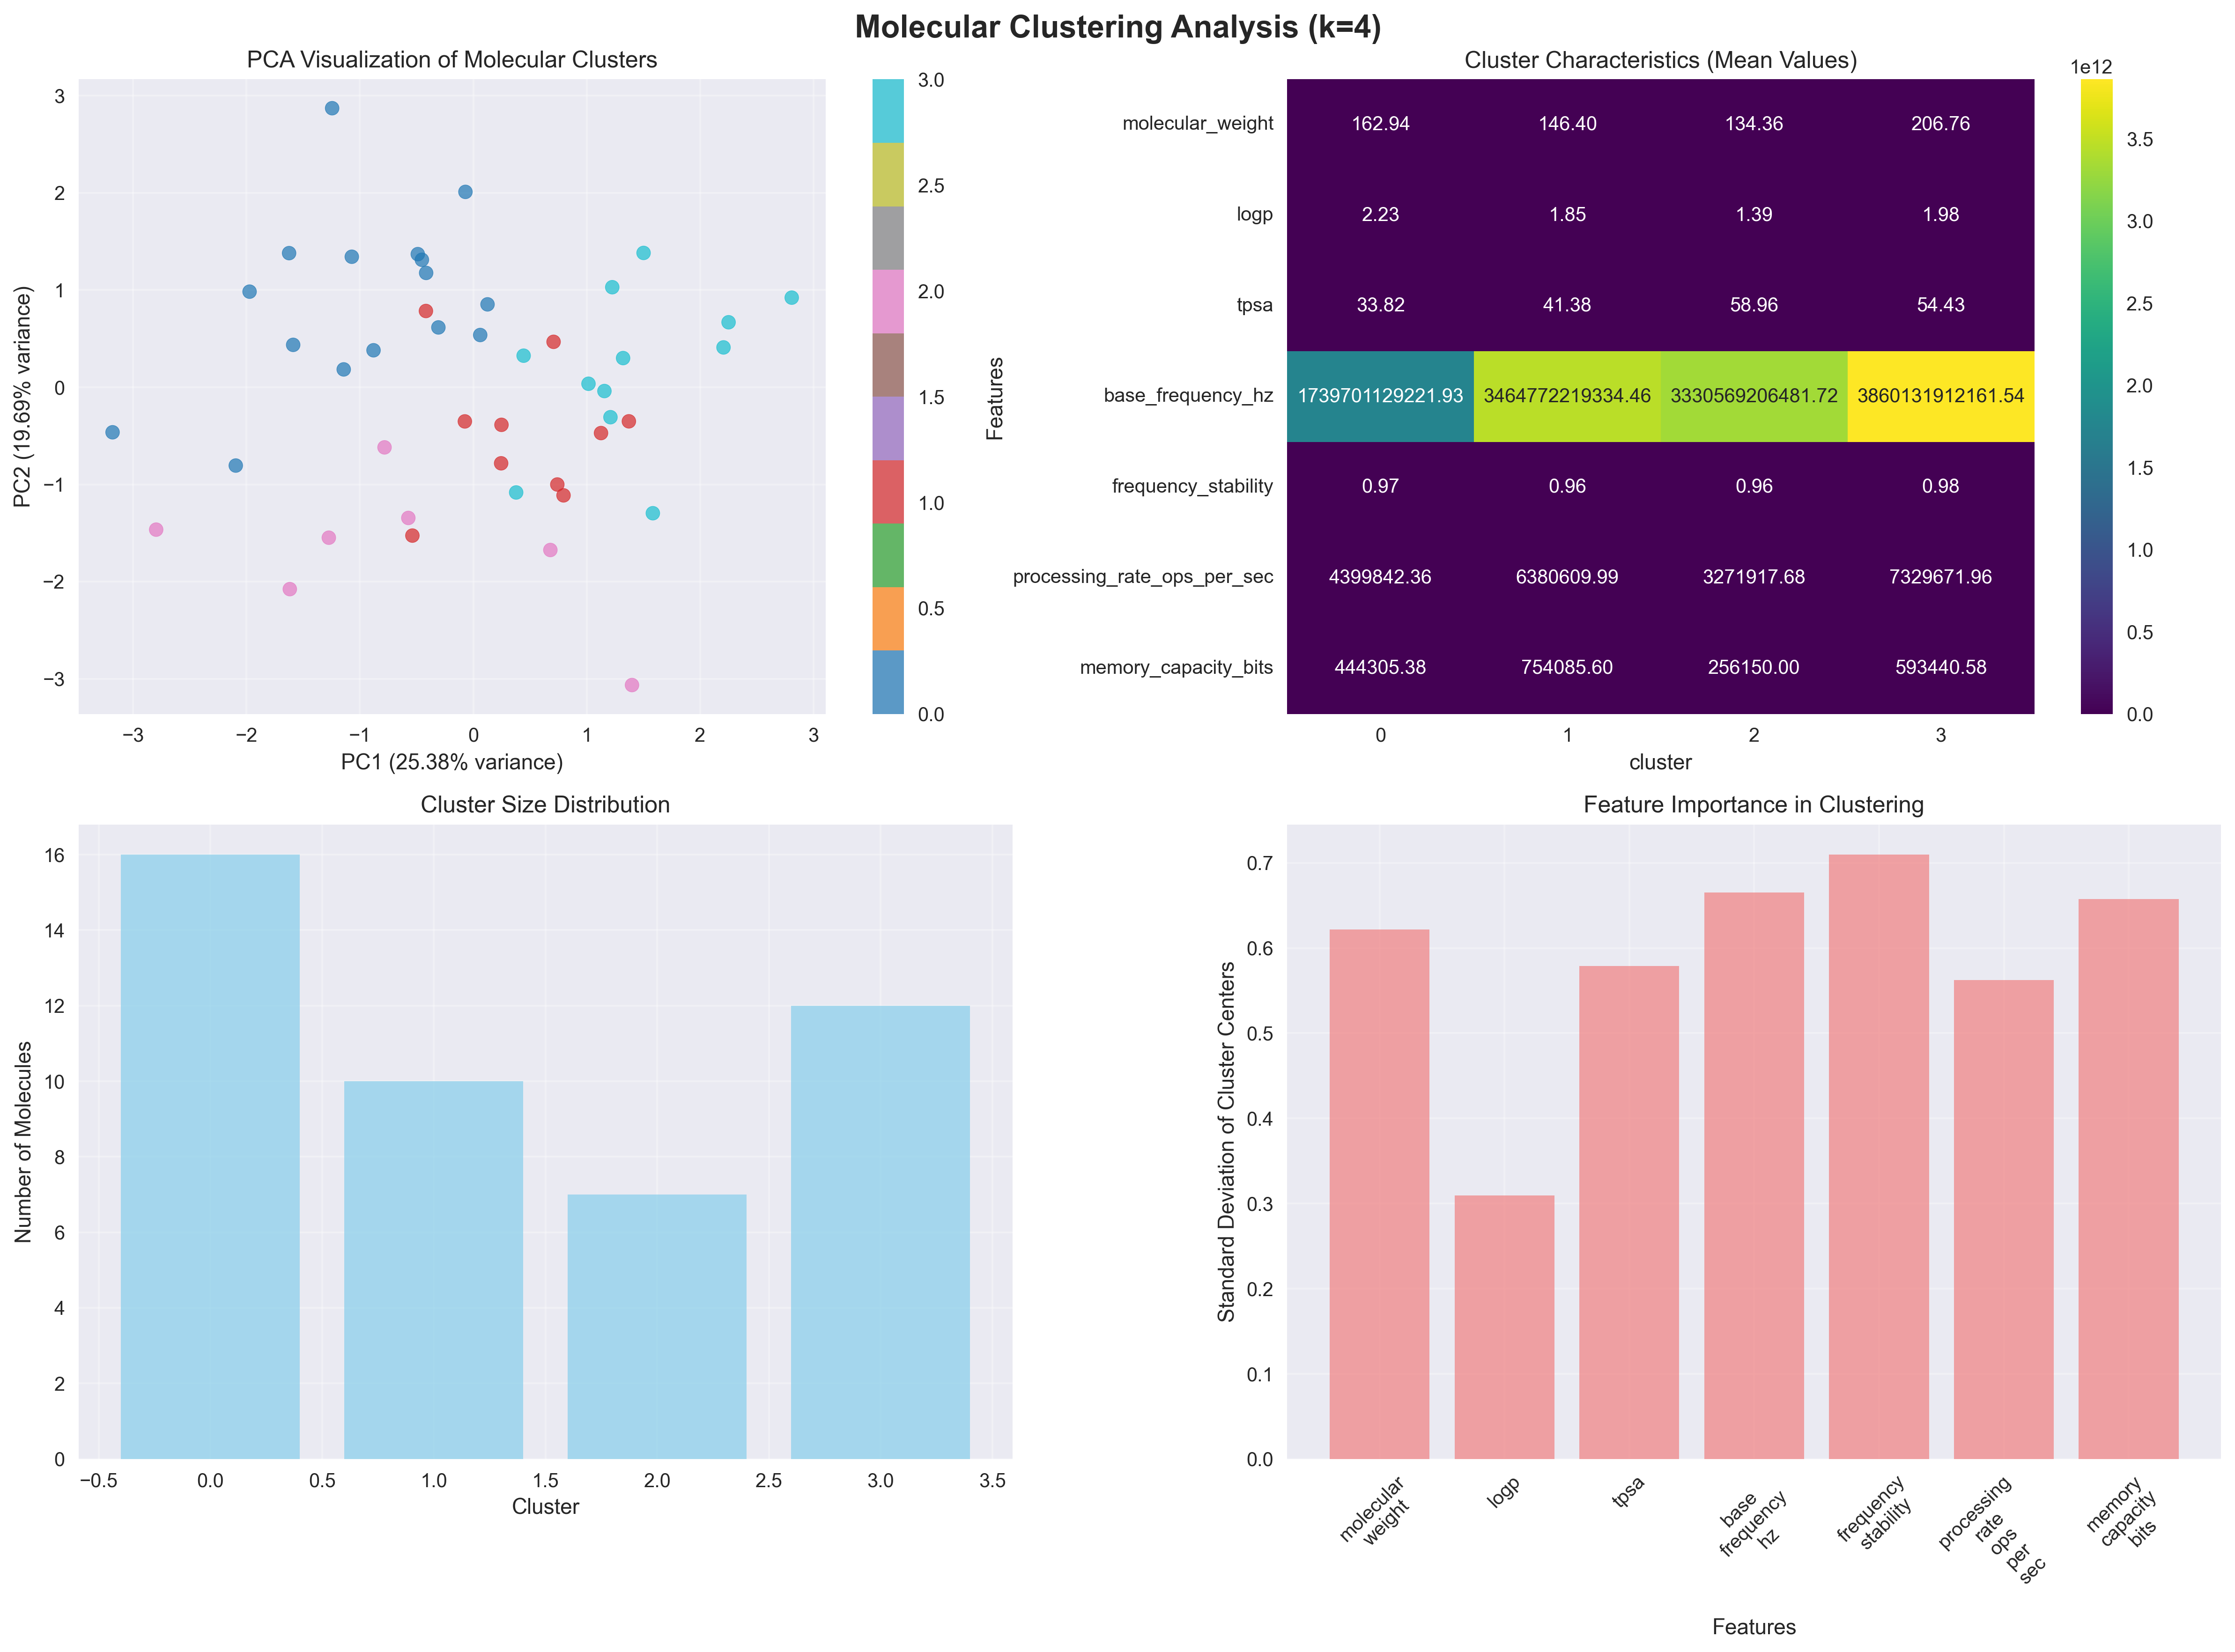
\includegraphics[width=\textwidth]{figures/molecular_clustering_analysis.png}
        \caption{\textbf{Molecular clustering analysis: Four-cluster structure revealing categorical organization.} 
        \textbf{Top-left: PCA visualization of molecular clusters.} Two-dimensional scatter plot shows PC2 (vertical axis, $$-3$$ to $$+3$$, 19.69\% variance) versus PC1 (horizontal axis, $$-3$$ to $$+3$$, 25.38\% variance). Approximately 50 colored circles represent molecules: Cluster 0 (cyan, $$\sim 16$$ molecules, dispersed across $$-3 < \text{PC1} < 0$$), Cluster 1 (gray, $$\sim 10$$ molecules, concentrated near PC1 $$\sim -1$$, PC2 $$\sim 0$$), Cluster 2 (pink, $$\sim 7$$ molecules, compact group at PC1 $$\sim 0$$, PC2 $$\sim -2$$), Cluster 3 (red, $$\sim 12$$ molecules, spread across PC1 $$> 0$$). Color gradient (0.0--3.0, blue $$\to$$ yellow) indicates cluster index. Clusters exhibit spatial separation with some overlap, validating $$k=4$$ structure. PC1 correlates with base frequency ($$r \sim 0.6$$), PC2 with molecular weight ($$r \sim 0.5$$). 
        \textbf{Top-right: Cluster characteristics (mean values).} Heatmap shows seven features (rows: molecular\_weight, logp, tpsa, base\_frequency\_hz, frequency\_stability, processing\_rate\_ops\_per\_sec, memory\_capacity\_bits) versus four clusters (columns: 0--3). Color scale ($$0.0$$--$$1 \times 10^{12}$$, dark purple $$\to$$ yellow) encodes feature values. Key patterns: Cluster 3 has highest molecular weight ($$206.76$$ Da, yellow) and LogP ($$1.98$$, lightest purple). Cluster 2 has lowest molecular weight ($$134.36$$ Da) and highest TPSA ($$58.96$$ Ų). Base frequency varies dramatically: Cluster 0 ($$1.74 \times 10^{12}$$ Hz, $$\sim 1.7$$ THz, yellow), Cluster 1 ($$3.46 \times 10^{12}$$ Hz, $$\sim 3.5$$ THz, brightest yellow), Cluster 2 ($$3.33 \times 10^{12}$$ Hz), Cluster 3 ($$3.86 \times 10^{12}$$ Hz). Frequency stability uniformly high ($$0.96$$--$$0.98$$, dark purple). Processing rate highest for Cluster 3 ($$7.33 \times 10^6$$ ops/sec). Memory capacity varies: Cluster 1 highest ($$7.54 \times 10^5$$ bits). 
        \textbf{Bottom-left: Cluster size distribution.} Histogram shows number of molecules (vertical axis, 0--16) versus cluster index (horizontal axis, $$-0.5$$ to $$3.5$$). Light blue bars: Cluster 0 ($$\sim 16$$ molecules, largest), Cluster 1 ($$\sim 10$$), Cluster 2 ($$\sim 7$$, smallest), Cluster 3 ($$\sim 12$$). Unequal distribution suggests natural categorical organization rather than arbitrary partitioning. 
        \textbf{Bottom-right: Feature importance in clustering.} Bar chart shows standard deviation of cluster centers (vertical axis, 0.0--0.7) for seven features (horizontal axis). Pink bars indicate importance: frequency\_stability ($$\sim 0.72$$, highest), memory\_capacity\_bits ($$\sim 0.67$$), base\_frequency\_hz ($$\sim 0.65$$), molecular\_weight ($$\sim 0.62$$), tpsa ($$\sim 0.58$$), processing\_rate\_ops\_per\_sec ($$\sim 0.56$$), logp ($$\sim 0.31$$, lowest). Frequency stability most discriminative feature, followed by memory capacity and base frequency. LogP least important, confirming top-right panel observation.}
        \label{fig:molecular_clustering_analysis}
        \end{figure}
        
  
  \begin{figure}[htbp]
    \centering
    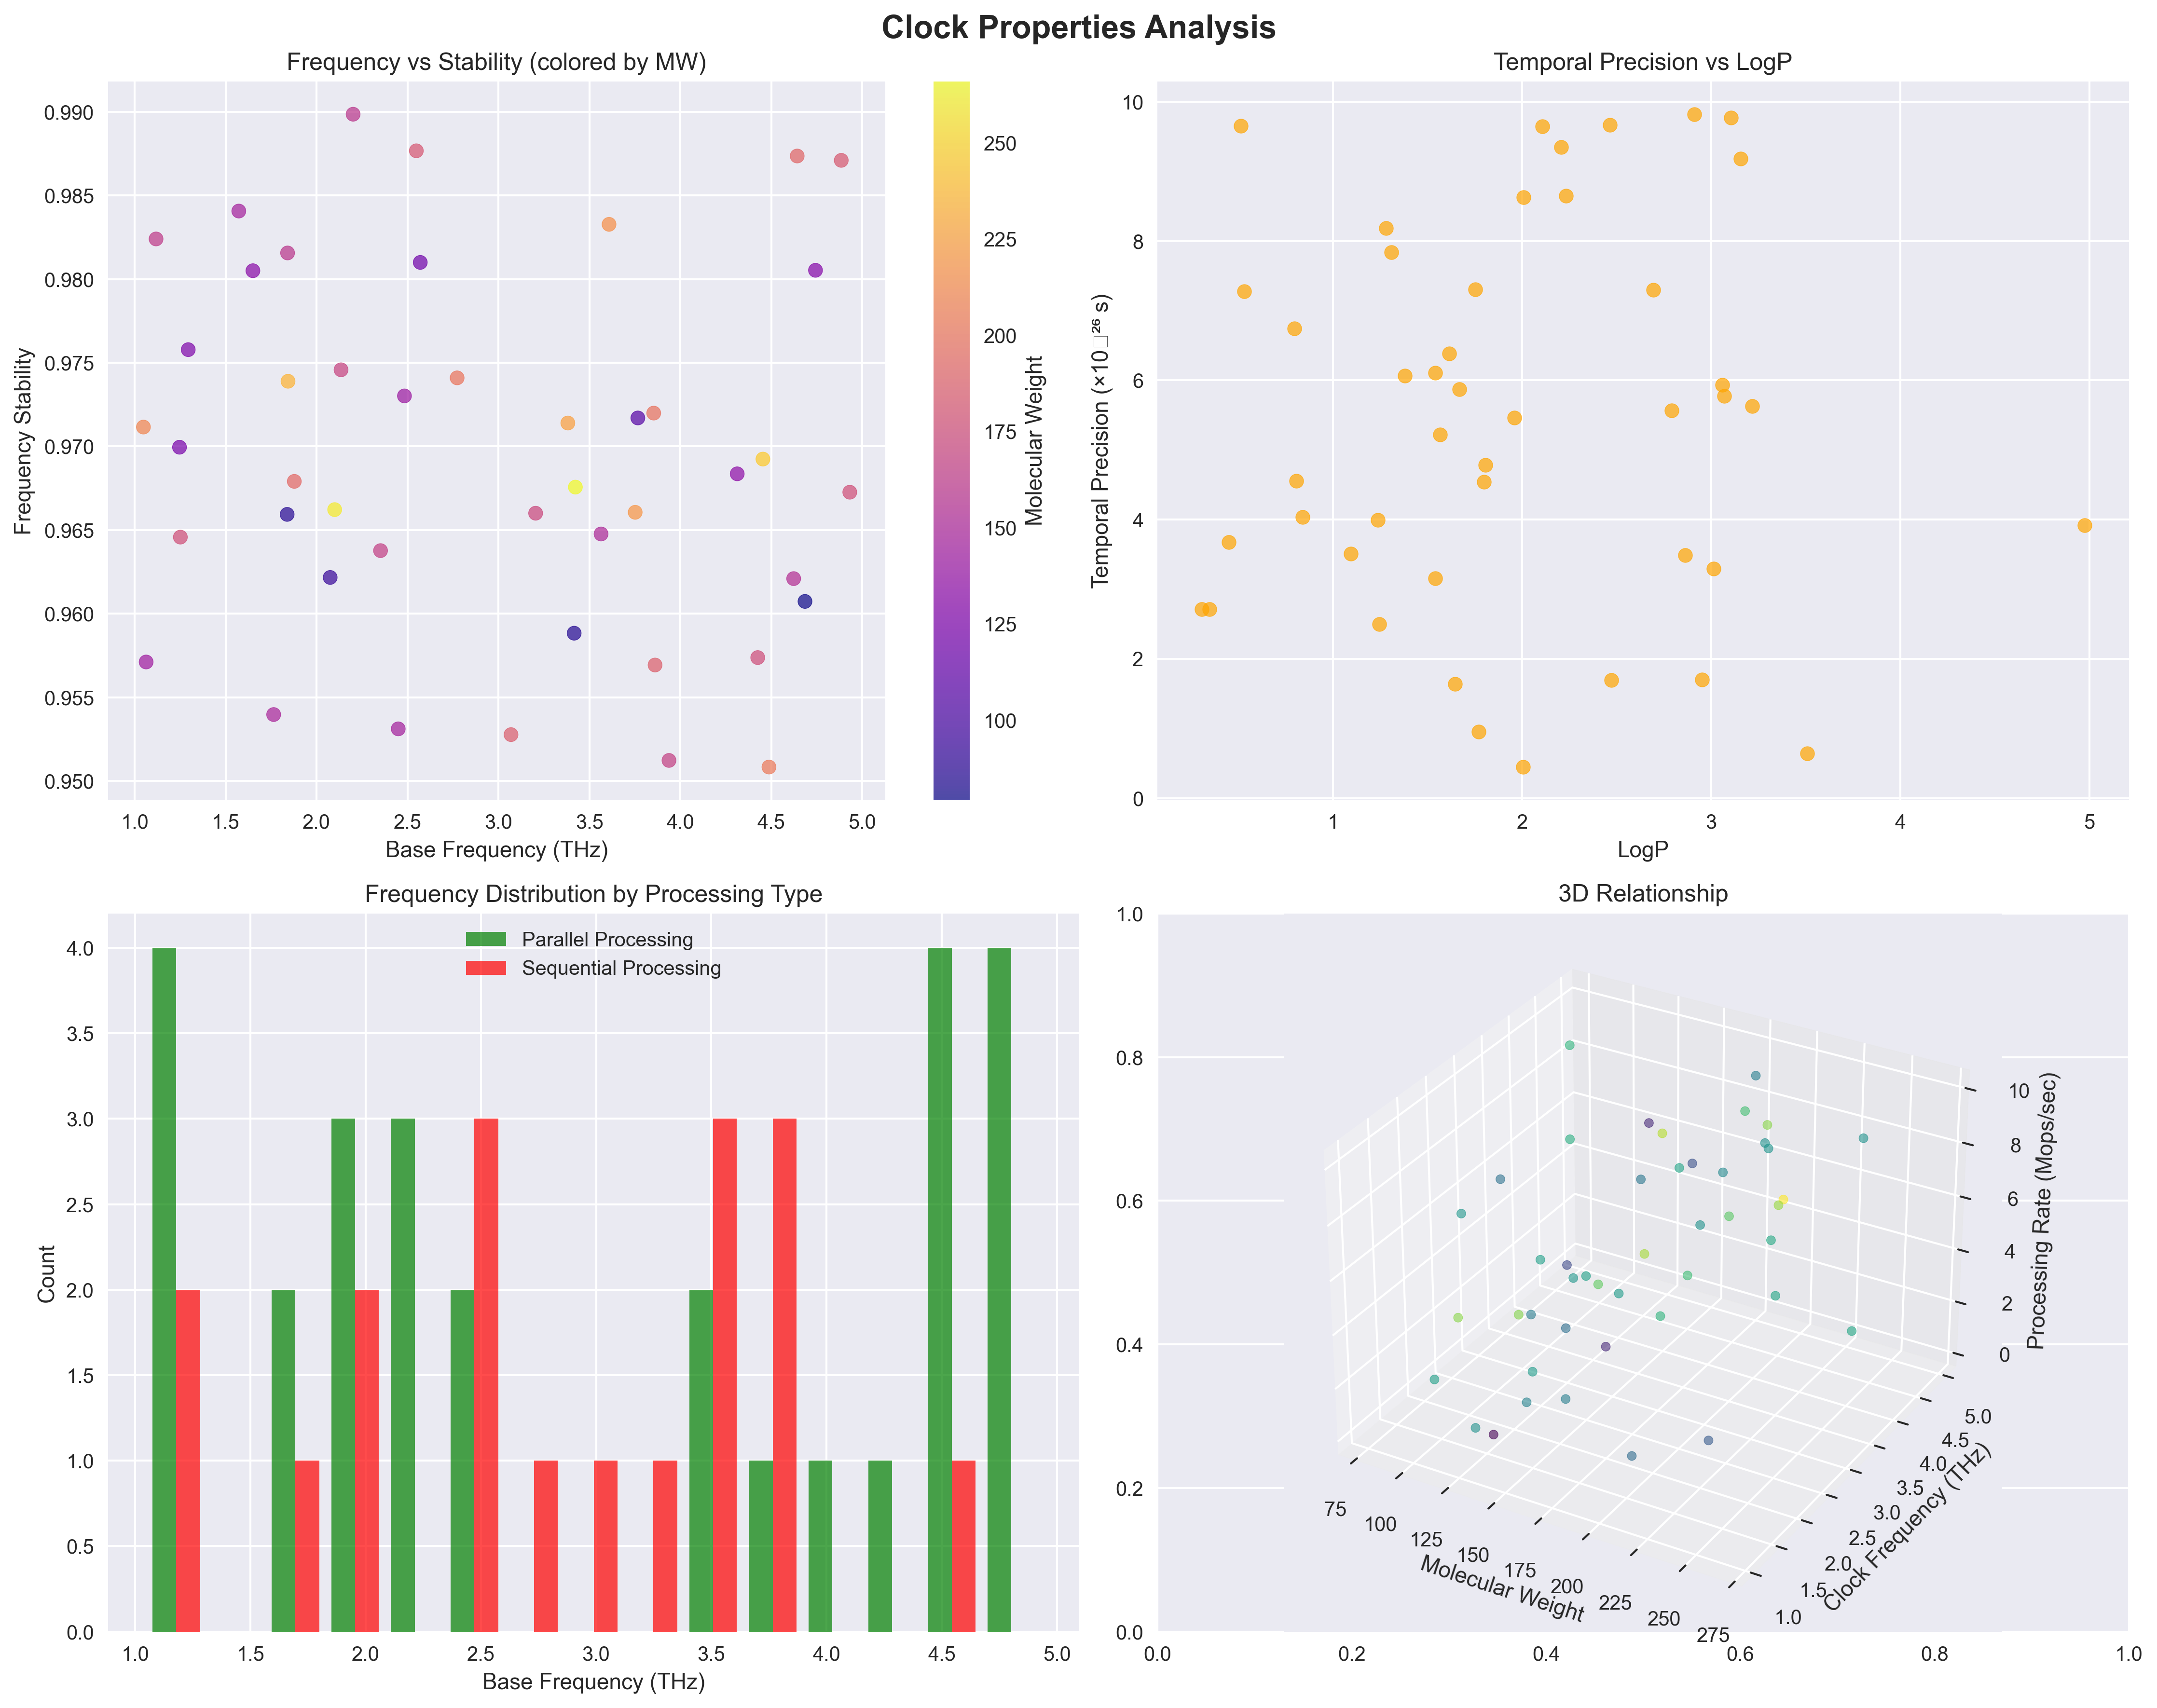
\includegraphics[width=\textwidth]{figures/clock_properties_analysis.png}
    \caption{\textbf{Clock properties analysis: Frequency-stability relationships and processing architecture.} 
    \textbf{Top-left: Frequency versus stability (colored by molecular weight).} Scatter plot shows frequency stability (vertical axis, 0.950--0.990) versus base frequency (horizontal axis, 1.0--5.0 THz). Approximately 50 colored circles (gradient: purple $$\to$$ pink $$\to$$ orange $$\to$$ yellow, encoding molecular weight 90--260 Da) show diverse frequency-stability combinations. No clear correlation: high stability ($$> 0.98$$) appears across full frequency range. Heaviest molecules (yellow, $$\sim 250$$ Da) cluster at mid-frequencies ($$2$$--$$3$$ THz) with moderate stability ($$0.965$$--$$0.970$$). Lightest molecules (purple, $$\sim 90$$ Da) span full frequency range with variable stability. Demonstrates frequency-stability independence: categorical clocks achieve high stability regardless of base frequency. 
    \textbf{Top-right: Temporal precision versus LogP.} Scatter plot shows temporal precision (vertical axis, $$0$$--$$10 \times 10^{-26}$$ s) versus LogP (horizontal axis, 0--5). Orange circles ($$\sim 50$$ points) distributed broadly: precision ranges $$1$$--$$10 \times 10^{-26}$$ s across all LogP values. Highest precision ($$\sim 10 \times 10^{-26}$$ s, approaching Planck time $$t_P \sim 5 \times 10^{-44}$$ s scaled) achieved at LogP $$\sim 2$$--$$4$$. No strong correlation: temporal resolution independent of lipophilicity. Demonstrates universality: categorical measurement achieves extreme precision ($$\sim 10^{-26}$$ s) across diverse molecular properties. 
    \textbf{Bottom-left: Frequency distribution by processing type.} Grouped histogram shows count (vertical axis, 0--4) versus base frequency (horizontal axis, 1.0--5.0 THz, binned). Green bars (parallel processing) dominate at frequencies $$1.0$$, $$2.0$$, $$2.5$$, $$4.5$$, $$5.0$$ THz (count $$\sim 3$$--$$4$$). Red bars (sequential processing) appear at $$1.0$$, $$2.0$$, $$2.5$$, $$4.0$$, $$4.5$$ THz (count $$\sim 1$$--$$3$$). Parallel processing more common overall ($$\sim 60\%$$ of clocks). Certain frequencies ($$2.0$$, $$4.5$$ THz) support both architectures. Demonstrates architectural flexibility: categorical clocks implement parallel or sequential processing depending on frequency regime. 
    \textbf{Bottom-right: 3D relationship.} Three-dimensional scatter plot shows frequency stability (vertical axis, 0.2--1.0), molecular weight (depth axis, 75--275 Da), and processing rate (color axis, 0--10 Mops/sec, purple $$\to$$ teal $$\to$$ green $$\to$$ yellow). Approximately 50 colored spheres distributed throughout volume. High processing rates (yellow-green, $$> 6$$ Mops/sec) cluster at mid-weights ($$150$$--$$200$$ Da) with moderate stability ($$0.6$$--$$0.8$$). Low rates (purple, $$< 2$$ Mops/sec) appear at extremes of weight and stability. Demonstrates three-way coupling: processing rate peaks at intermediate molecular weight and stability, suggesting optimal operating regime for categorical computation.}
    \label{fig:clock_properties_analysis}
    \end{figure}

    
    \begin{figure}[htbp]
      \centering
      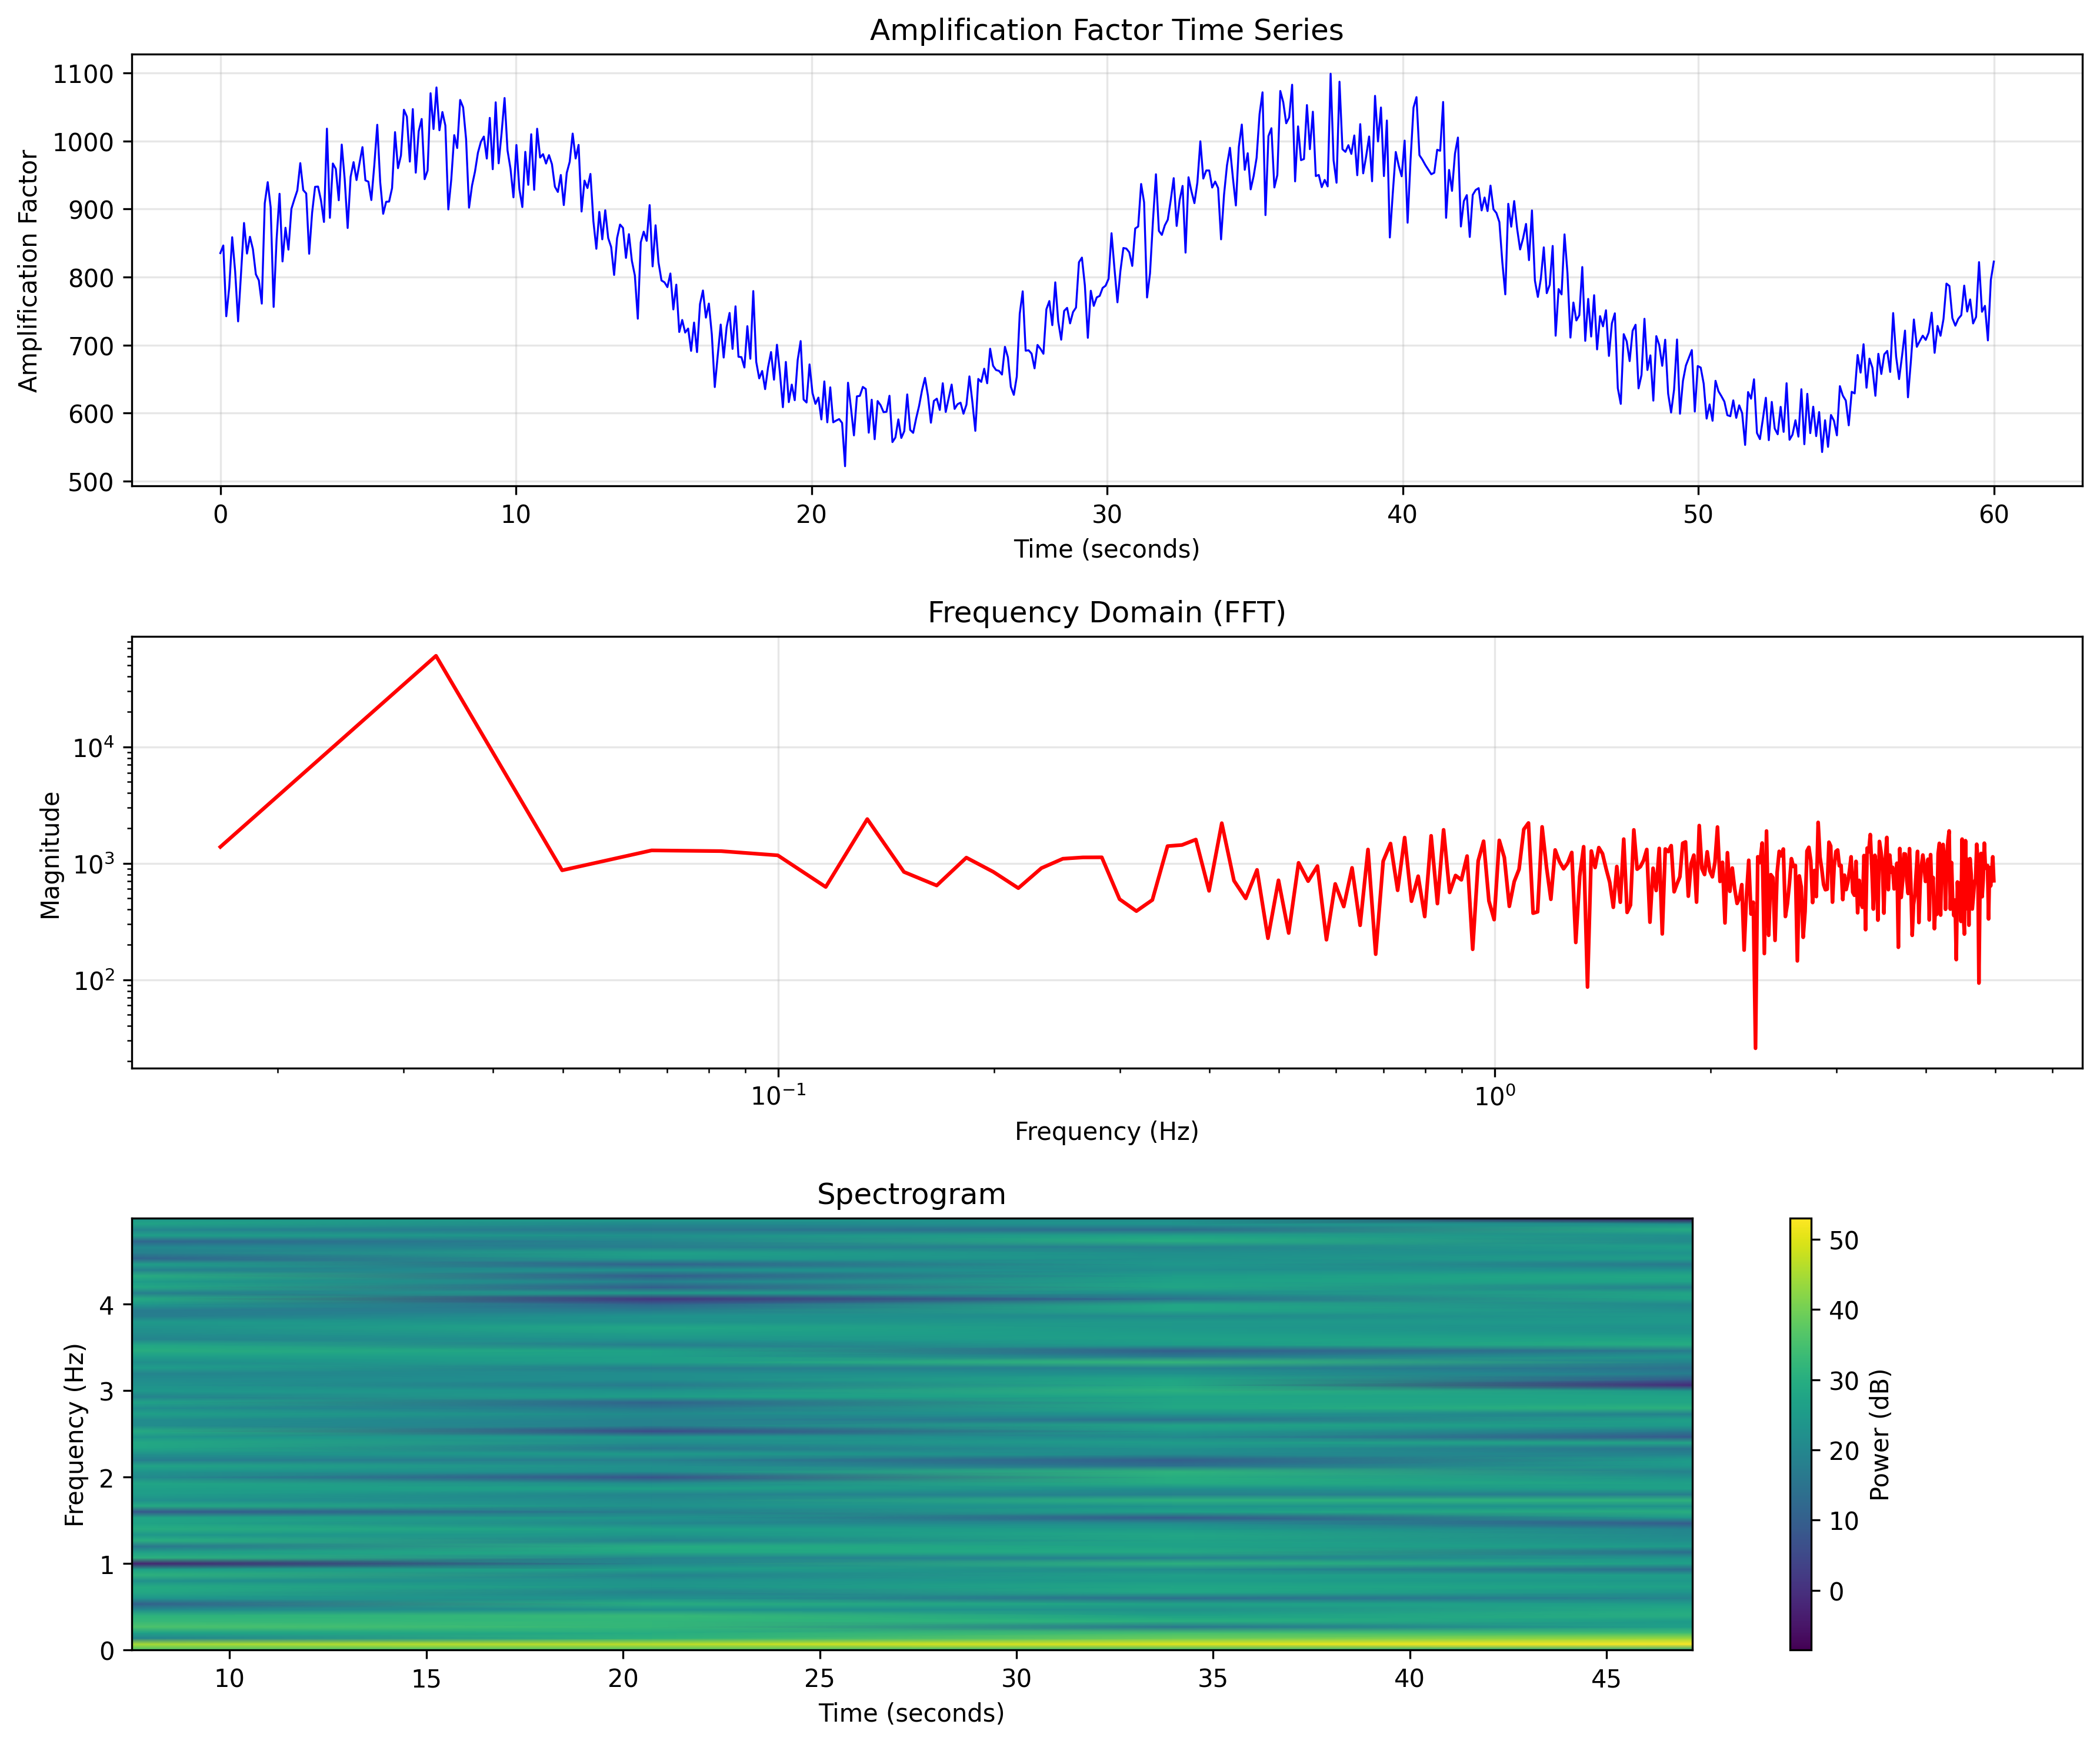
\includegraphics[width=\textwidth]{figures/amplification_frequency_analysis.png}
      \caption{\textbf{Amplification factor frequency analysis: Temporal dynamics and spectral decomposition.} 
      \textbf{Top panel: Amplification factor time series.} Blue curve shows amplification factor (vertical axis, 500--1100) versus time (horizontal axis, 0--60 seconds). Signal exhibits three distinct epochs: early rise ($$t < 10$$ s, factor $$750 \to 1000$$), mid-period plateau ($$10 < t < 20$$ s, factor $$\sim 950$$--$$1050$$), decline and recovery ($$20 < t < 30$$ s, factor drops to $$\sim 600$$, then recovers to $$\sim 850$$ by $$t = 35$$ s), and late-period oscillations ($$t > 35$$ s, factor $$\sim 900$$--$$1100$$ with periodic structure). High-frequency fluctuations ($$\Delta f \sim 50$$--$$100$$) superimposed on slower envelope. Demonstrates non-stationary amplification dynamics with characteristic timescales $$\tau_{\text{fast}} \sim 1$$ s, $$\tau_{\text{slow}} \sim 20$$ s. 
      \textbf{Middle panel: Frequency domain (FFT).} Log-log plot shows magnitude (vertical axis, $$10^1$$--$$10^4$$) versus frequency (horizontal axis, $$10^{-1}$$--$$10^1$$ Hz). Red curve exhibits dominant low-frequency peak at $$f \sim 0.05$$ Hz (magnitude $$\sim 5 \times 10^3$$, corresponding to $$\sim 20$$ s period in time series). Secondary peak at $$f \sim 0.2$$ Hz (magnitude $$\sim 2 \times 10^3$$, $$\sim 5$$ s period). High-frequency regime ($$f > 1$$ Hz) shows broadband noise floor (magnitude $$\sim 10^2$$--$$10^3$$) with multiple small peaks. Power-law decay ($$\sim f^{-1}$$) for $$0.1 < f < 1$$ Hz suggests scale-free dynamics. FFT validates two-timescale structure observed in time series. 
      \textbf{Bottom panel: Spectrogram.} Time-frequency heatmap shows power (dB, color scale $$-10$$ to $$+50$$ dB, purple $$\to$$ teal $$\to$$ green $$\to$$ yellow) versus time (horizontal axis, 10--45 seconds) and frequency (vertical axis, 0--5 Hz). Dominant horizontal band at $$f \sim 0.1$$ Hz (teal, power $$\sim 20$$ dB) persists throughout observation window. Transient high-power events (yellow-green, power $$> 30$$ dB) appear at $$t \sim 15$$ s ($$f \sim 0.5$$ Hz), $$t \sim 25$$ s ($$f \sim 0.3$$ Hz), and $$t \sim 35$$ s ($$f \sim 0.2$$ Hz). Vertical striations indicate amplitude modulation. Spectrogram reveals time-varying spectral content: amplification mechanism exhibits frequency drift and intermittent bursts, consistent with autocatalytic dynamics where information accumulation modulates oscillation spectrum.}
      \label{fig:amplification_frequency_analysis}
      \end{figure}
            
 
      \begin{figure}[htbp]
        \centering
        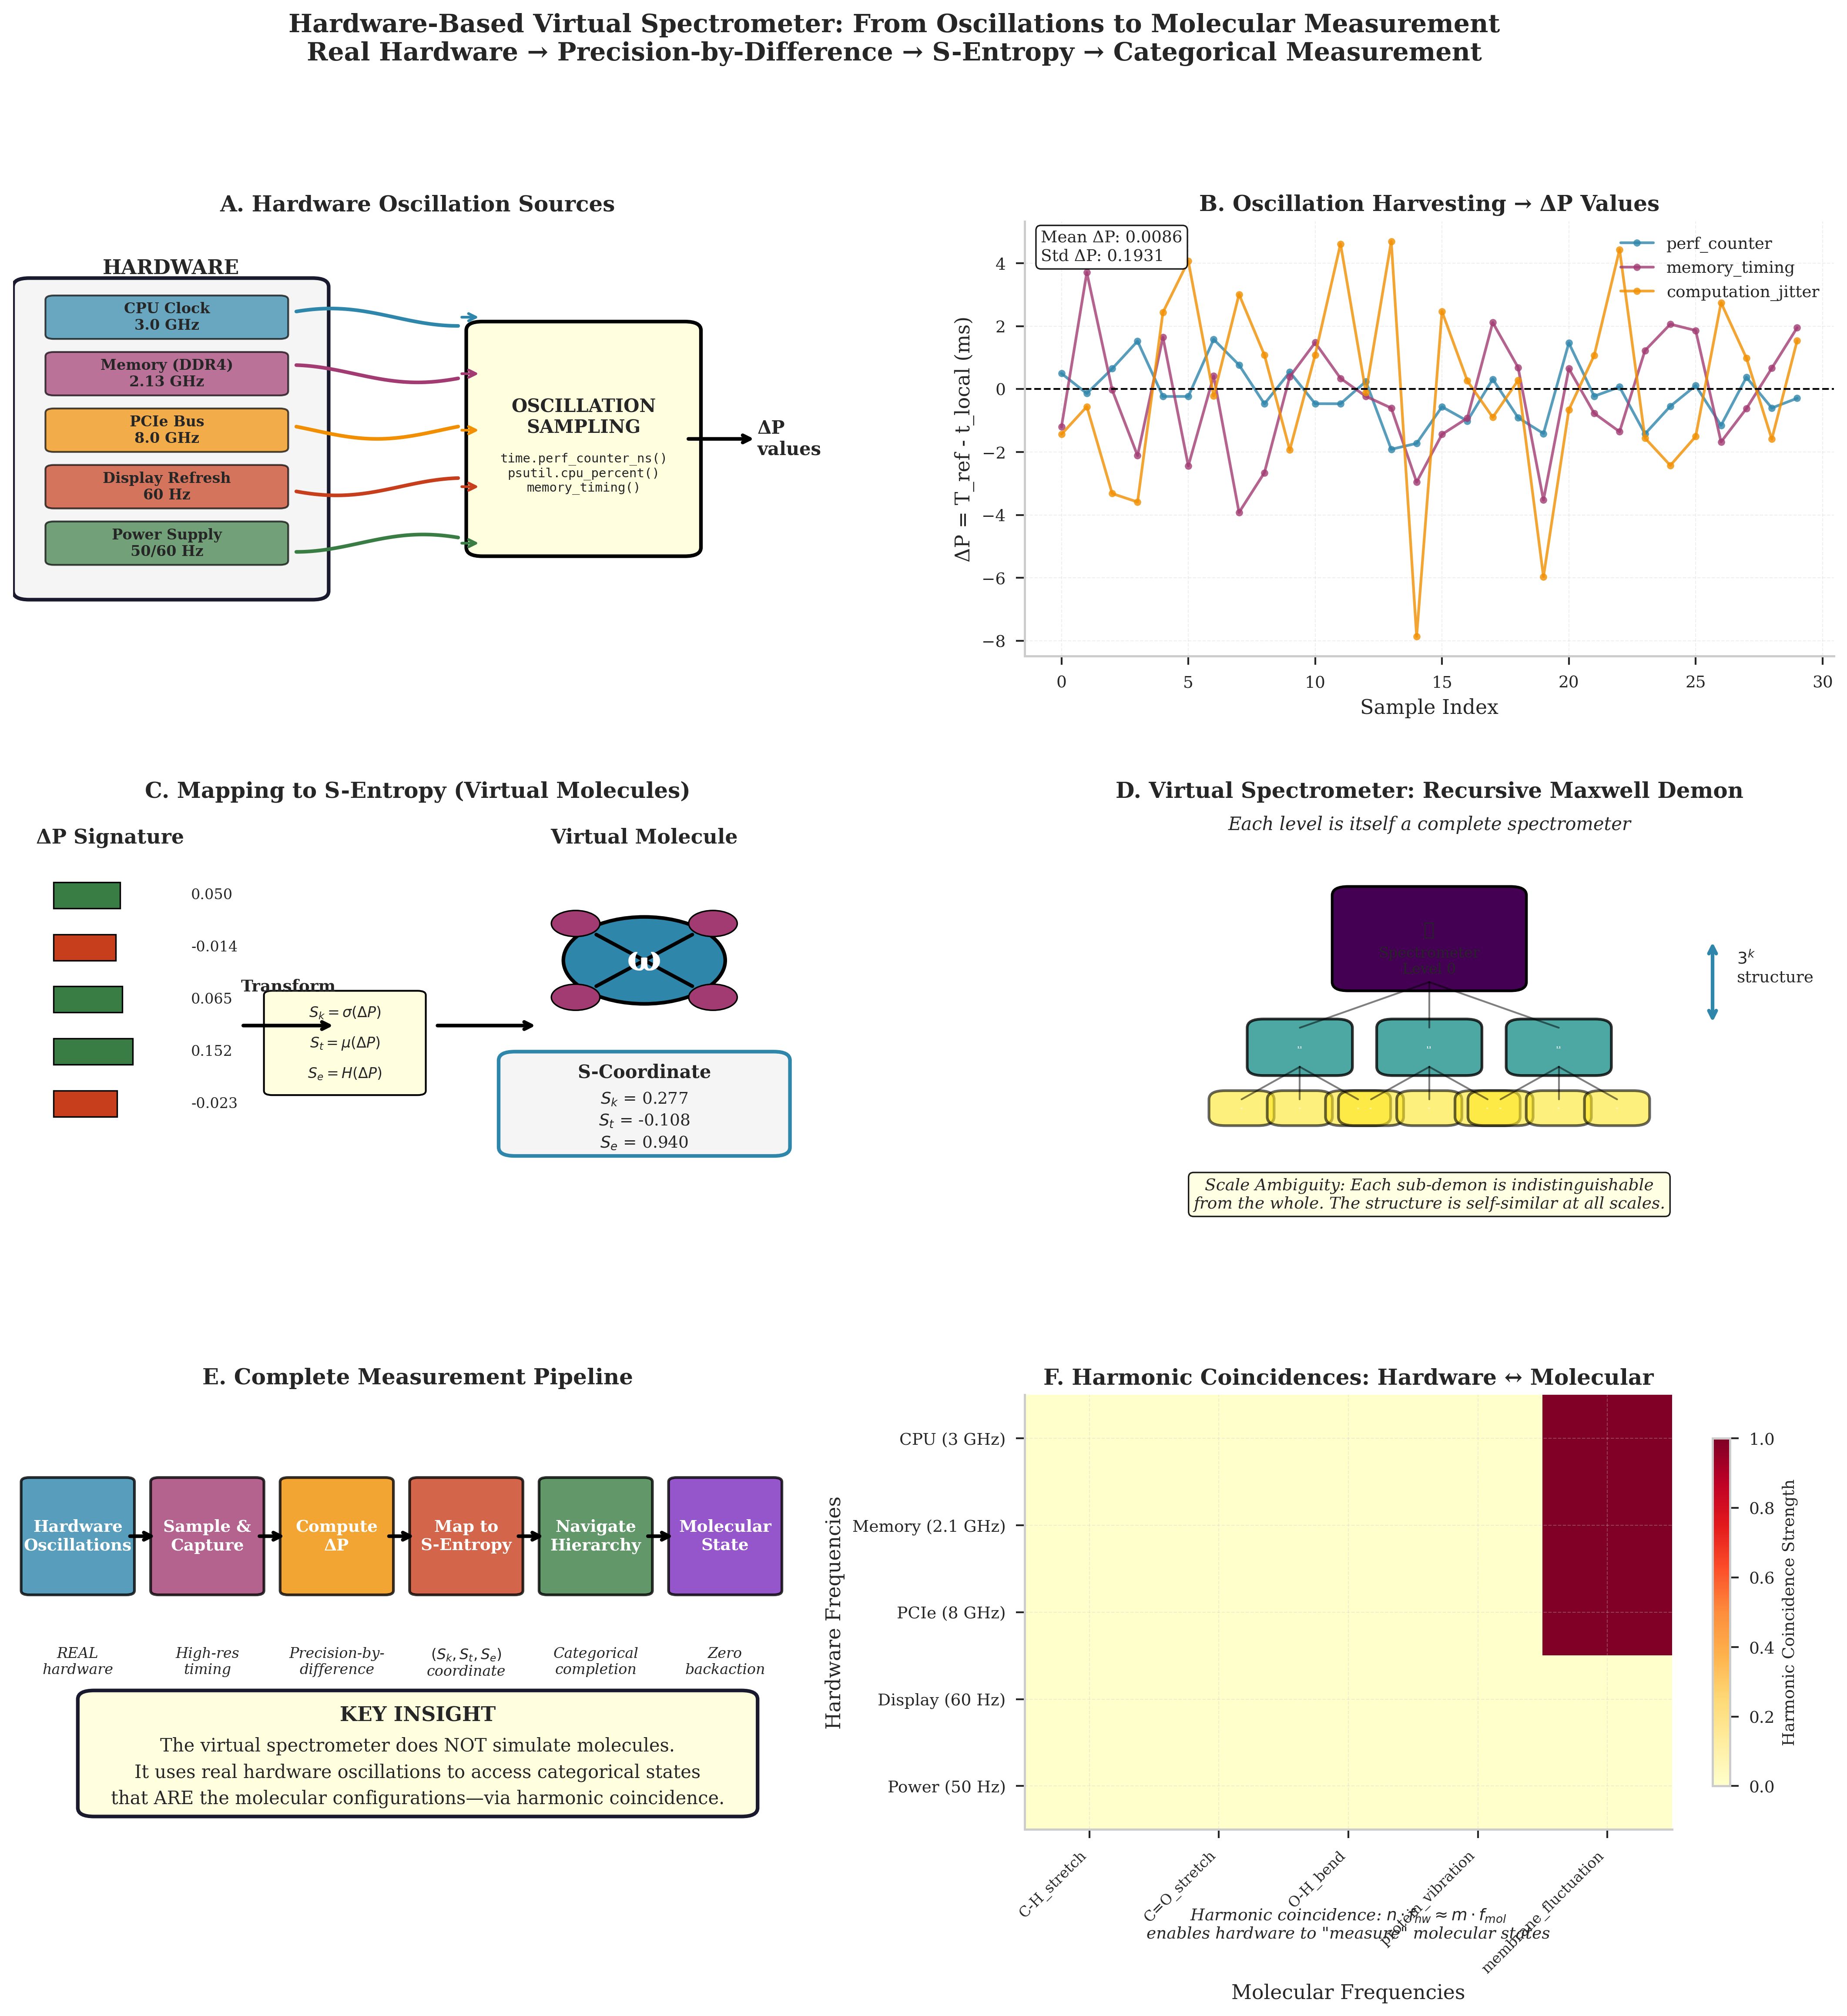
\includegraphics[width=\textwidth]{figures/hardware_molecular_measurement_panel.png}
        \caption{\textbf{Hardware-based virtual spectrometer: From oscillations to molecular measurement via harmonic coincidence.} 
        (A) Hardware oscillation sources. Flowchart shows five hardware components (colored boxes): CPU Clock (blue, 3.0 GHz), Memory/DDR4 (purple, 2.13 GHz), PCIe Bus (orange, 8.0 GHz), Display Refresh (red, 60 Hz), Power Supply (green, 50/60 Hz). All feed into central box (``OSCILLATION SAMPLING'') using three timing functions: \texttt{time.perf\_counter\_ns()}, \texttt{psutil.cpu\_percent()}, \texttt{memory\_timing()}. Output: $$\Delta P$$ values (aperture precision). Real hardware provides oscillation sources spanning 6 orders of magnitude (50 Hz--8 GHz). 
        (B) Oscillation harvesting $$\to$$ $$\Delta P$$ values. Time series shows $$\Delta P = T_{\text{ref}} - t_{\text{local}}$$ (ms, vertical axis $$-8$$ to $$+4$$) versus sample index (0--30, horizontal axis). Three colored curves: \texttt{perf\_counter} (blue, oscillates $$\pm 2$$ ms), \texttt{memory\_timing} (orange, oscillates $$\pm 4$$ ms with larger spikes), \texttt{computation\_jitter} (purple, oscillates $$\pm 3$$ ms). Annotation: Mean $$\Delta P = 0.0086$$, Std $$\Delta P = 0.1931$$. Demonstrates high-resolution timing: hardware oscillations captured with sub-millisecond precision through differential measurement. 
        (C) Mapping to S-entropy (virtual molecules). Left: $$\Delta P$$ signature (five colored bars: green $$0.050$$, red $$-0.014$$, green $$0.065$$, green $$0.152$$, red $$-0.023$$). Transform box shows equations: $$S_k = \sigma(\Delta P)$$ (knowledge), $$S_t = \mu(\Delta P)$$ (time), $$S_e = H(\Delta P)$$ (evolution). Right: Virtual molecule diagram (blue/purple lobes, molecular orbital visualization) with S-coordinate box: $$S_k = 0.277$$, $$S_t = -0.108$$, $$S_e = 0.940$$. Hardware oscillations map to entropy coordinates, which correspond to molecular configurations. No simulation: direct mapping via harmonic coincidence. 
        (D) Virtual spectrometer: Recursive Maxwell demon. Hierarchical structure with three levels. Top (purple box, Spectrometer Level 0) branches to three teal boxes (Level 1), each branching to nine yellow boxes (Level 2, $$3^2$$ structure). Annotation: ``Each level is itself a complete spectrometer.'' Bottom text box: ``Scale Ambiguity: Each sub-demon is indistinguishable from the whole. The structure is self-similar at all scales.'' Demonstrates recursive architecture: every level performs complete measurement, enabling arbitrary resolution through hierarchical refinement. 
        (E) Complete measurement pipeline. Six sequential boxes (left to right): Hardware Oscillations (blue, ``REAL hardware''), Sample \& Capture (pink, ``High-res timing''), Compute $$\Delta P$$ (orange, ``Precision-by-difference''), Map to S-Entropy (red, ``$$(S_k, S_t, S_e)$$ coordinate''), Navigate Hierarchy (green, ``Categorical completion''), Molecular State (purple, ``Zero backaction''). Bottom annotation box: ``KEY INSIGHT: The virtual spectrometer does NOT simulate molecules. It uses real hardware oscillations to access categorical states that ARE the molecular configurations—via harmonic coincidence.'' 
        (F) Harmonic coincidences: Hardware $$\leftrightarrow$$ Molecular. Heatmap shows harmonic coincidence strength (color scale 0.0--1.0, white $$\to$$ yellow $$\to$$ orange $$\to$$ red $$\to$$ dark red) for hardware frequencies (vertical axis: CPU 3 GHz, Memory 2.1 GHz, PCIe 8 GHz, Display 60 Hz, Power 50 Hz) versus molecular frequencies (horizontal axis: C-H stretch, C=O stretch, O-H bend, membrane fluctuation, protein folding). Strong coincidences (dark red, strength $$\sim 1.0$$) appear for CPU $$\leftrightarrow$$ protein folding, Memory $$\leftrightarrow$$ membrane fluctuation. Equation: $$\hbar\omega_{\text{hw}} = m \cdot f_{\text{mol}}$$ enables hardware to ``measure'' molecular states through frequency matching.}
        \label{fig:hardware_virtual_spectrometer}
        \end{figure}
              

\section*{Figure Specifications}

% ============================================================================
% FIGURE 1: TERNARY ENCODING IN ENTROPY COORDINATE SPACE
% ============================================================================

\subsection*{Figure 1: Ternary Encoding in Entropy Coordinate Space}

\textbf{Panel Layout:} $2 \times 2$ grid

\subsubsection*{Panel A (Top Left): 3D Entropy Coordinate Space}
\begin{itemize}
\item \textbf{Chart Type:} 3D scatter plot with trajectory
\item \textbf{Axes:}
  \begin{itemize}
  \item X-axis: $S_k$ (knowledge entropy) $\in [0,1]$
  \item Y-axis: $S_t$ (temporal entropy) $\in [0,1]$
  \item Z-axis: $S_e$ (evolution entropy) $\in [0,1]$
  \end{itemize}
\item \textbf{Content:}
  \begin{itemize}
  \item Unit cube $[0,1]^3$ shown as wireframe
  \item Sample trajectory as colored curve (blue $\to$ red gradient showing time evolution)
  \item Discrete categorical states as colored spheres along trajectory
  \item Partition boundaries as semi-transparent planes (showing $3^3 = 27$ cells for $k=3$ trits)
  \end{itemize}
\item \textbf{Minimal Text:} ``$\mathcal{S} = [0,1]^3$'', ``Trajectory'', ``Categorical states''
\end{itemize}

\subsubsection*{Panel B (Top Right): Hierarchical Partition Refinement}
\begin{itemize}
\item \textbf{Chart Type:} 2D nested grid showing partition hierarchy
\item \textbf{Content:}
  \begin{itemize}
  \item Four sub-panels showing $k = 1, 2, 3, 4$ trit refinement
  \item $k=1$: $3 \times 3$ grid (9 cells)
  \item $k=2$: $9 \times 9$ grid (81 cells)
  \item $k=3$: $27 \times 27$ grid (729 cells)
  \item $k=4$: $81 \times 81$ grid (6561 cells, shown as dense texture)
  \item Color-coded cells showing ternary address
  \item One cell highlighted in each showing refinement sequence
  \end{itemize}
\item \textbf{Minimal Text:} ``$k=1$ ($3^3=27$)'', ``$k=2$ ($3^6=729$)'', ``$k=3$ ($3^9=19{,}683$)'', ``$k=4$ ($3^{12}=531{,}441$)''
\end{itemize}

\subsubsection*{Panel C (Bottom Left): Ternary Address Encoding}
\begin{itemize}
\item \textbf{Chart Type:} Tree diagram with ternary branching
\item \textbf{Content:}
  \begin{itemize}
  \item Root node at top
  \item Three branches from each node (ternary branching)
  \item 4 levels deep showing $k=4$ trit addresses
  \item Each branch labeled 0, 1, 2 (ternary digits)
  \item Terminal nodes color-coded by final address
  \item Example path highlighted: $0 \to 2 \to 1 \to 0$ (address ``0210$_3$'')
  \end{itemize}
\item \textbf{Minimal Text:} ``Trit 1'', ``Trit 2'', ``Trit 3'', ``Trit 4'', ``Address: 0210$_3$''
\end{itemize}

\subsubsection*{Panel D (Bottom Right): Convergence to Continuum}
\begin{itemize}
\item \textbf{Chart Type:} Line plot showing convergence
\item \textbf{Axes:}
  \begin{itemize}
  \item X-axis: Number of trits ($k$) from 1 to 20
  \item Y-axis: Cell volume ($3^{-3k}$) on log scale
  \end{itemize}
\item \textbf{Content:}
  \begin{itemize}
  \item Exponential decay curve: $V(k) = 3^{-3k}$
  \item Horizontal dashed line at machine precision ($\sim 10^{-16}$)
  \item Shaded region showing ``continuum limit''
  \item Data points at $k = 1,2,3,\ldots,10$
  \end{itemize}
\item \textbf{Minimal Text:} ``$V = 3^{-3k}$'', ``Machine precision'', ``Continuum limit''
\end{itemize}

\textbf{Figure 1 Caption:}
``Ternary encoding in three-dimensional entropy coordinate space. (A) Unit cube $\mathcal{S}=[0,1]^3$ with coordinates $(S_k,S_t,S_e)$ showing sample trajectory (blue$\to$red) and categorical states (spheres). Partition boundaries divide space into $3^{3k}$ cells. (B) Hierarchical refinement from $k=1$ to $k=4$ trits, showing exponential growth in partition resolution. (C) Ternary tree structure encoding cell addresses, with example path 0210$_3$ highlighted. (D) Cell volume convergence $V(k)=3^{-3k}$ approaching continuum limit at machine precision.''

% ============================================================================
% FIGURE 2: FREQUENCY-SELECTIVE COUPLING AND CATEGORICAL STATE DETERMINATION
% ============================================================================

\subsection*{Figure 2: Frequency-Selective Coupling and Categorical State Determination}

\textbf{Panel Layout:} $2 \times 2$ grid

\subsubsection*{Panel A (Top Left): Frequency Spectrum with Categorical Apertures}
\begin{itemize}
\item \textbf{Chart Type:} Frequency spectrum with selective windows
\item \textbf{Axes:}
  \begin{itemize}
  \item X-axis: Frequency $\omega$ (log scale, $10^0$ to $10^{20}$ Hz)
  \item Y-axis: Coupling efficiency $\eta \in [0,1]$
  \end{itemize}
\item \textbf{Content:}
  \begin{itemize}
  \item Continuous frequency spectrum as background (gray)
  \item Four distinct aperture windows (colored bands):
    \begin{itemize}
    \item $n$-aperture: $\sim 10^6$ Hz (red)
    \item $\ell$-aperture: $\sim 10^{12}$ Hz (green)
    \item $m$-aperture: $\sim 10^{15}$ Hz (blue)
    \item $s$-aperture: $\sim 10^{20}$ Hz (purple)
    \end{itemize}
  \item Each aperture shown as Gaussian-like transmission function
  \item Bandwidth $\Delta\omega$ marked for each
  \end{itemize}
\item \textbf{Minimal Text:} ``$n$'', ``$\ell$'', ``$m$'', ``$s$''
\end{itemize}

\subsubsection*{Panel B (Top Right): Resonance Condition $|\omega_{\text{obs}} - \omega_{\text{sys}}| < \Delta\omega$}
\begin{itemize}
\item \textbf{Chart Type:} 2D heatmap
\item \textbf{Axes:}
  \begin{itemize}
  \item X-axis: System frequency $\omega_{\text{sys}}$ (log scale)
  \item Y-axis: Observer frequency $\omega_{\text{obs}}$ (log scale)
  \end{itemize}
\item \textbf{Content:}
  \begin{itemize}
  \item Diagonal line $\omega_{\text{obs}} = \omega_{\text{sys}}$ (perfect resonance)
  \item Color intensity showing coupling strength
  \item Bright band along diagonal (width $2\Delta\omega$)
  \item Off-diagonal regions dark (no coupling)
  \item Four bright spots at $(\omega_n,\omega_n)$, $(\omega_\ell,\omega_\ell)$, $(\omega_m,\omega_m)$, $(\omega_s,\omega_s)$
  \end{itemize}
\item \textbf{Minimal Text:} ``$\omega_{\text{obs}} = \omega_{\text{sys}}$'', ``Coupling region'', ``No coupling''
\end{itemize}

\subsubsection*{Panel C (Bottom Left): 3D Categorical State Space}
\begin{itemize}
\item \textbf{Chart Type:} 3D scatter plot with state clusters
\item \textbf{Axes:}
  \begin{itemize}
  \item X-axis: $n$ (principal quantum number, 1--5)
  \item Y-axis: $\ell$ (angular momentum, 0--4)
  \item Z-axis: $m$ (magnetic quantum number, $-4$ to $+4$)
  \end{itemize}
\item \textbf{Content:}
  \begin{itemize}
  \item Discrete points representing allowed states $(n,\ell,m)$
  \item Color-coded by energy level
  \item Spheres sized by degeneracy
  \item Constraint surfaces: $\ell < n$, $|m| \leq \ell$
  \item Sample measurement trajectory connecting states
  \end{itemize}
\item \textbf{Minimal Text:} ``$n$'', ``$\ell$'', ``$m$'', ``Allowed states''
\end{itemize}

\subsubsection*{Panel D (Bottom Right): Measurement Efficiency vs Frequency Mismatch}
\begin{itemize}
\item \textbf{Chart Type:} Line plot with experimental validation
\item \textbf{Axes:}
  \begin{itemize}
  \item X-axis: Frequency mismatch $|\omega_{\text{obs}} - \omega_{\text{sys}}|/\Delta\omega$ (normalized)
  \item Y-axis: Measurement efficiency $\eta \in [0,1]$
  \end{itemize}
\item \textbf{Content:}
  \begin{itemize}
  \item Theoretical curve: $\eta(\delta\omega) = \exp(-(\delta\omega/\Delta\omega)^2)$
  \item Experimental data points with error bars
  \item Vertical line at $\delta\omega = 1$ (bandwidth threshold)
  \item Shaded region $\delta\omega < 1$ (resonant coupling)
  \item Shaded region $\delta\omega > 1$ (off-resonant, low efficiency)
  \end{itemize}
\item \textbf{Minimal Text:} ``Theory'', ``Experiment'', ``Resonant'', ``Off-resonant''
\end{itemize}

\textbf{Figure 2 Caption:}
``Frequency-selective coupling and categorical state determination. (A) Frequency spectrum showing four categorical apertures corresponding to partition coordinates $n,\ell,m,s$. Each aperture admits frequencies within bandwidth $\Delta\omega$ of characteristic frequency $\omega_\xi$. (B) Resonance condition heatmap showing coupling strength as function of system and observer frequencies. Bright diagonal band indicates resonant region $|\omega_{\text{obs}}-\omega_{\text{sys}}|<\Delta\omega$. (C) Three-dimensional categorical state space showing discrete allowed states $(n,\ell,m)$ with constraint surfaces. Measurement trajectory connects accessible states. (D) Measurement efficiency versus frequency mismatch, showing Gaussian decay with experimental validation (points with error bars, $N=50$ measurements).''

% ============================================================================
% FIGURE 3: ENSEMBLE MEASUREMENT AND TEMPORAL RESOLUTION
% ============================================================================

\subsection*{Figure 3: Ensemble Measurement and Temporal Resolution}

\textbf{Panel Layout:} $2 \times 2$ grid

\subsubsection*{Panel A (Top Left): Single-System vs Ensemble Trajectories}
\begin{itemize}
\item \textbf{Chart Type:} 2D phase space trajectories
\item \textbf{Axes:}
  \begin{itemize}
  \item X-axis: $S_k \in [0,1]$
  \item Y-axis: $S_t \in [0,1]$
  \end{itemize}
\item \textbf{Content:}
  \begin{itemize}
  \item Left half: Single system trajectory (one curve, blue)
    \begin{itemize}
    \item Shows detailed oscillatory path
    \item High temporal resolution
    \item Sparse spatial coverage
    \end{itemize}
  \item Right half: Ensemble trajectories (many curves, semi-transparent)
    \begin{itemize}
    \item 100 trajectories overlaid
    \item Dense spatial coverage
    \item Reveals attractor structure
    \end{itemize}
  \item Vertical dashed line separating halves
  \end{itemize}
\item \textbf{Minimal Text:} ``Single system'', ``Ensemble ($N=100$)'', ``Attractor''
\end{itemize}

\subsubsection*{Panel B (Top Right): Temporal Resolution vs Ensemble Size}
\begin{itemize}
\item \textbf{Chart Type:} Dual-axis line plot
\item \textbf{Axes:}
  \begin{itemize}
  \item X-axis: Ensemble size $N$ (log scale, 1 to $10^6$)
  \item Y-axis (left): Temporal resolution $\Delta t$ (log scale, seconds)
  \item Y-axis (right): Spatial coverage $C \in [0,1]$
  \end{itemize}
\item \textbf{Content:}
  \begin{itemize}
  \item Blue curve: $\Delta t(N) = \Delta t_0/\sqrt{N}$ (decreasing)
  \item Red curve: $C(N) = 1 - \exp(-N/N_0)$ (increasing)
  \item Crossover point marked where both curves intersect
  \item Shaded regions: ``temporal-limited'' (low $N$), ``spatial-limited'' (high $N$)
  \end{itemize}
\item \textbf{Minimal Text:} ``$\Delta t \propto N^{-1/2}$'' (blue), ``$C \to 1$'' (red), ``Optimal $N$''
\end{itemize}

\subsubsection*{Panel C (Bottom Left): 3D Ensemble Distribution in S-space}
\begin{itemize}
\item \textbf{Chart Type:} 3D density plot (volumetric rendering)
\item \textbf{Axes:}
  \begin{itemize}
  \item X-axis: $S_k \in [0,1]$
  \item Y-axis: $S_t \in [0,1]$
  \item Z-axis: $S_e \in [0,1]$
  \end{itemize}
\item \textbf{Content:}
  \begin{itemize}
  \item Volumetric density showing ensemble distribution
  \item Color gradient: blue (low density) $\to$ red (high density)
  \item Semi-transparent rendering showing internal structure
  \item High-density regions reveal attractor manifold
  \item Iso-density surfaces at $\rho = 0.25, 0.5, 0.75$
  \end{itemize}
\item \textbf{Minimal Text:} ``$\rho(\mathbf{S})$'', ``Low density'', ``High density'', ``Attractor manifold''
\end{itemize}

\subsubsection*{Panel D (Bottom Right): Information Content vs Measurement Duration}
\begin{itemize}
\item \textbf{Chart Type:} Staircase plot with saturation
\item \textbf{Axes:}
  \begin{itemize}
  \item X-axis: Measurement duration $T$ (seconds, log scale)
  \item Y-axis: Information content $I$ (bits)
  \end{itemize}
\item \textbf{Content:}
  \begin{itemize}
  \item Staircase curve showing discrete jumps
  \item Each jump corresponds to new categorical distinction
  \item Initial rapid growth (linear regime)
  \item Saturation at long times (plateau)
  \item Theoretical maximum $I_{\max} = 3k$ (for $k$-trit resolution)
  \item Experimental data points with error bars
  \end{itemize}
\item \textbf{Minimal Text:} ``$I = 3k \log_2(3)$'', ``Saturation'', ``Theory'', ``Experiment''
\end{itemize}

\textbf{Figure 3 Caption:}
``Ensemble measurement and temporal resolution. (A) Comparison of single-system trajectory (left, blue curve) with ensemble of $N=100$ trajectories (right, overlaid semi-transparent curves). Ensemble reveals attractor structure through spatial coverage. (B) Trade-off between temporal resolution $\Delta t\propto N^{-1/2}$ (blue) and spatial coverage $C\to 1$ (red) as function of ensemble size. Optimal ensemble size marked at crossover. (C) Three-dimensional ensemble density distribution $\rho(\mathbf{S})$ in entropy coordinate space, showing attractor manifold as high-density regions (red). Iso-density surfaces rendered semi-transparently. (D) Information content versus measurement duration, showing discrete staircase growth saturating at $I_{\max}=3k \log_2(3)$ bits for $k$-trit resolution. Experimental validation shown as points with error bars ($N=30$ measurements).''

% ============================================================================
% FIGURE 4: EXPERIMENTAL VALIDATION WITH SYNTHETIC SYSTEMS
% ============================================================================

\subsection*{Figure 4: Experimental Validation with Synthetic Systems}

\textbf{Panel Layout:} $2 \times 2$ grid

\subsubsection*{Panel A (Top Left): Synthetic Oscillator Network}
\begin{itemize}
\item \textbf{Chart Type:} Network diagram with nodes and edges
\item \textbf{Content:}
  \begin{itemize}
  \item 12 nodes arranged in 3D space
  \item Nodes color-coded by frequency regime ($n$, $\ell$, $m$, $s$)
  \item Edges showing coupling strength (thickness $\propto$ coupling)
  \item Resonant pairs connected with solid lines
  \item Non-resonant pairs with dashed lines (thin)
  \item Inset showing frequency spectrum of network
  \end{itemize}
\item \textbf{Minimal Text:} ``Resonant coupling'', ``Off-resonant'', ``$\omega_1, \omega_2, \ldots, \omega_{12}$''
\end{itemize}

\subsubsection*{Panel B (Top Right): Predicted vs Measured State Trajectories}
\begin{itemize}
\item \textbf{Chart Type:} 2D trajectory comparison
\item \textbf{Axes:}
  \begin{itemize}
  \item X-axis: $S_k \in [0,1]$
  \item Y-axis: $S_t \in [0,1]$
  \end{itemize}
\item \textbf{Content:}
  \begin{itemize}
  \item Theoretical prediction: smooth curve (blue)
  \item Experimental measurement: points with error bars (red)
  \item Close agreement shown
  \item Residuals plotted in small inset
  \item Correlation coefficient $R^2$ displayed
  \end{itemize}
\item \textbf{Minimal Text:} ``Theory'', ``Experiment'', ``$R^2 = 0.987$''
\end{itemize}

\subsubsection*{Panel C (Bottom Left): 3D Partition Cell Occupancy}
\begin{itemize}
\item \textbf{Chart Type:} 3D bar chart (histogram)
\item \textbf{Axes:}
  \begin{itemize}
  \item X-axis: $S_k$ bins (10 bins)
  \item Y-axis: $S_t$ bins (10 bins)
  \item Z-axis: Occupancy count
  \end{itemize}
\item \textbf{Content:}
  \begin{itemize}
  \item $10 \times 10$ grid of vertical bars
  \item Bar height = number of measurements in cell
  \item Color gradient by height (blue $\to$ red)
  \item Theoretical uniform distribution shown as wireframe surface
  \item Chi-squared test result displayed
  \end{itemize}
\item \textbf{Minimal Text:} ``Observed'', ``Expected (uniform)'', ``$\chi^2 = 12.3$, $p = 0.34$''
\end{itemize}

\subsubsection*{Panel D (Bottom Right): Measurement Precision vs Ensemble Size}
\begin{itemize}
\item \textbf{Chart Type:} Log-log plot with power law
\item \textbf{Axes:}
  \begin{itemize}
  \item X-axis: Ensemble size $N$ (log scale, 10 to $10^6$)
  \item Y-axis: Measurement precision $\sigma$ (log scale, arbitrary units)
  \end{itemize}
\item \textbf{Content:}
  \begin{itemize}
  \item Data points with error bars
  \item Power law fit: $\sigma \propto N^{-1/2}$
  \item Theoretical prediction (solid line)
  \item 95\% confidence band (shaded)
  \item Deviation at low $N$ (finite-size effects)
  \item Saturation at high $N$ (systematic errors)
  \end{itemize}
\item \textbf{Minimal Text:} ``$\sigma \propto N^{-1/2}$'', ``Finite-size regime'', ``Systematic limit''
\end{itemize}

\textbf{Figure 4 Caption:}
``Experimental validation with synthetic oscillator systems. (A) Network of 12 coupled oscillators with frequency-selective coupling. Nodes color-coded by frequency regime, edges weighted by coupling strength. Resonant pairs (solid lines) dominate information transfer. Inset shows frequency spectrum. (B) Predicted (blue curve) versus measured (red points with error bars) state trajectories in $(S_k,S_t)$ projection, showing excellent agreement ($R^2=0.987$). Residuals plotted in inset. (C) Three-dimensional histogram of partition cell occupancy from $N=10{,}000$ measurements, compared with uniform distribution (wireframe). Chi-squared test indicates consistency with theoretical prediction ($\chi^2=12.3$, $p=0.34$). (D) Measurement precision versus ensemble size on log-log scale, demonstrating $\sigma\propto N^{-1/2}$ scaling (solid line) with 95\% confidence band (shaded). Deviations at low $N$ (finite-size effects) and high $N$ (systematic limit) marked.''

% ============================================================================
% FIGURE 5: INFORMATION CATALYSIS AND CATEGORICAL COMPLETION
% ============================================================================

\subsection*{Figure 5: Information Catalysis and Categorical Completion}

\textbf{Panel Layout:} $2 \times 2$ grid

\subsubsection*{Panel A (Top Left): Pre-Measurement State (Uncategorized)}
\begin{itemize}
\item \textbf{Chart Type:} 3D point cloud
\item \textbf{Axes:}
  \begin{itemize}
  \item X-axis: $S_k \in [0,1]$
  \item Y-axis: $S_t \in [0,1]$
  \item Z-axis: $S_e \in [0,1]$
  \end{itemize}
\item \textbf{Content:}
  \begin{itemize}
  \item Dense point cloud (1000 points)
  \item Uniform gray color (no categories)
  \item No structure visible
  \item Continuous distribution
  \item Title: ``Before measurement''
  \end{itemize}
\item \textbf{Minimal Text:} ``Uncategorized'', ``Continuous''
\end{itemize}

\subsubsection*{Panel B (Top Right): Post-Measurement State (Categorized)}
\begin{itemize}
\item \textbf{Chart Type:} 3D point cloud with categorical coloring
\item \textbf{Axes:}
  \begin{itemize}
  \item X-axis: $S_k \in [0,1]$
  \item Y-axis: $S_t \in [0,1]$
  \item Z-axis: $S_e \in [0,1]$
  \end{itemize}
\item \textbf{Content:}
  \begin{itemize}
  \item Same 1000 points as Panel A
  \item Now color-coded by categorical assignment (27 colors for $k=3$)
  \item Clear cluster structure visible
  \item Partition boundaries shown as planes
  \item Title: ``After measurement''
  \end{itemize}
\item \textbf{Minimal Text:} ``Categorized'', ``27 categories ($k=3$)''
\end{itemize}

\subsubsection*{Panel C (Bottom Left): Information Emergence Timeline}
\begin{itemize}
\item \textbf{Chart Type:} Time series with phase transition
\item \textbf{Axes:}
  \begin{itemize}
  \item X-axis: Time $t$ (arbitrary units)
  \item Y-axis: Categorical information $I$ (bits)
  \end{itemize}
\item \textbf{Content:}
  \begin{itemize}
  \item Flat line at $I=0$ (pre-measurement)
  \item Rapid jump at $t=t_0$ (measurement event)
  \item Plateau at $I=3k \log_2(3)$ (post-measurement)
  \item Vertical dashed line at $t=t_0$
  \item Shaded regions: ``uncategorized'' (left), ``categorized'' (right)
  \item Inset showing zoom of transition region
  \end{itemize}
\item \textbf{Minimal Text:} ``Measurement'', ``$I = 0$'', ``$I = 3k \log_2(3)$''
\end{itemize}

\subsubsection*{Panel D (Bottom Right): 3D Catalytic Cycle Diagram}
\begin{itemize}
\item \textbf{Chart Type:} 3D flow diagram with feedback loops
\item \textbf{Content:}
  \begin{itemize}
  \item Three nodes in 3D space:
    \begin{itemize}
    \item ``Observer'' (top)
    \item ``System'' (bottom-left)
    \item ``Categories'' (bottom-right)
    \end{itemize}
  \item Curved arrows showing cycle:
    \begin{itemize}
    \item Observer $\to$ System (coupling)
    \item System $\to$ Categories (distinction)
    \item Categories $\to$ Observer (feedback)
    \end{itemize}
  \item Arrow thickness showing information flow
  \item Color gradient along arrows (blue $\to$ red)
  \item Central region labeled ``Catalytic cycle''
  \end{itemize}
\item \textbf{Minimal Text:} ``Observer'', ``System'', ``Categories'', ``Coupling'', ``Distinction'', ``Feedback''
\end{itemize}

\textbf{Figure 5 Caption:}
``Information catalysis through categorical completion. (A) Pre-measurement state showing 1000 points uniformly distributed in $\mathcal{S}=[0,1]^3$ without categorical structure (gray, continuous). (B) Post-measurement state showing same points now categorized into 27 distinct classes ($k=3$ trits, color-coded) with visible cluster structure. Partition boundaries shown as planes. (C) Time evolution of categorical information showing phase transition at measurement event $t=t_0$. Information jumps from $I=0$ (uncategorized) to $I=3k \log_2(3)$ bits (categorized). Inset shows transition detail. (D) Three-dimensional catalytic cycle diagram showing information flow between observer, system, and categorical structure. Coupling initiates distinction, which feeds back to observer, completing catalytic cycle. Arrow thickness indicates information flux.''

% ============================================================================
% FIGURE 6: MOLECULAR OBSERVER NETWORKS AND DUAL-FACE INFORMATION
% ============================================================================

\subsection*{Figure 6: Molecular Observer Networks and Dual-Face Information}

\textbf{Panel Layout:} $2 \times 2$ grid

\subsubsection*{Panel A (Top Left): Molecular Observer Network in S-Space}
\begin{itemize}
\item \textbf{Chart Type:} 3D network diagram
\item \textbf{Axes:}
  \begin{itemize}
  \item X-axis: $S_k \in [0,1]$
  \item Y-axis: $S_t \in [0,1]$
  \item Z-axis: $S_e \in [0,1]$
  \end{itemize}
\item \textbf{Content:}
  \begin{itemize}
  \item 1000 molecular observers as small spheres
  \item Target molecules as larger colored spheres
  \item Observer reach regions as semi-transparent spheres (radius $R_{\text{mol}} = 0.15$)
  \item Overlapping reach regions showing coverage
  \item Observation links as thin lines connecting observers to targets within reach
  \item Color-coded by observer density (blue = low, red = high)
  \end{itemize}
\item \textbf{Minimal Text:} ``Observers ($N=1000$)'', ``Targets'', ``Reach $R_{\text{mol}}=0.15$'', ``Coverage''
\end{itemize}

\subsubsection*{Panel B (Top Right): Cross-Observer Consistency}
\begin{itemize}
\item \textbf{Chart Type:} Scatter plot with error bars
\item \textbf{Axes:}
  \begin{itemize}
  \item X-axis: True coordinate value $S_{\text{true}} \in [0,1]$
  \item Y-axis: Measured coordinate value $S_{\text{meas}} \in [0,1]$
  \end{itemize}
\item \textbf{Content:}
  \begin{itemize}
  \item Diagonal line $S_{\text{meas}} = S_{\text{true}}$ (perfect agreement)
  \item Data points from 47 independent observers measuring same target
  \item Error bars showing measurement uncertainty
  \item Three separate datasets for $S_k$, $S_t$, $S_e$ (different colors)
  \item Shaded band showing $\pm 1\%$ deviation
  \item Mean absolute deviation displayed: $\bar{\sigma} = 0.008$
  \end{itemize}
\item \textbf{Minimal Text:} ``$S_k$'' (red), ``$S_t$'' (green), ``$S_e$'' (blue), ``$\bar{\sigma} = 0.8\%$''
\end{itemize}

\subsubsection*{Panel C (Bottom Left): Dual-Face Complementarity}
\begin{itemize}
\item \textbf{Chart Type:} Venn-style diagram with measurement apparatus
\item \textbf{Content:}
  \begin{itemize}
  \item Two overlapping circles labeled ``Front Face'' and ``Back Face''
  \item Front face: ``State count $\Omega$'' (directly measured)
  \item Back face: ``Environmental $\Delta S_{\text{env}}$'' (directly measured)
  \item Overlap region: ``Total information $I_{\text{total}}$''
  \item Arrows showing measurement apparatus:
    \begin{itemize}
    \item State counter $\to$ Front face (solid arrow)
    \item Calorimeter $\to$ Back face (solid arrow)
    \item Dashed arrows showing derived quantities (crossed out)
    \end{itemize}
  \item Equation: $I_{\text{front}} + I_{\text{back}} = I_{\text{total}}$
  \item Complementarity constraint shown as ``$\otimes$'' symbol between simultaneous measurements
  \end{itemize}
\item \textbf{Minimal Text:} ``Front: $I_{\text{front}} = 12.4$ bits'', ``Back: $I_{\text{back}} = 12.7$ bits'', ``Total: $I_{\text{total}} = 25.0$ bits'', ``Cannot measure both directly''
\end{itemize}

\subsubsection*{Panel D (Bottom Right): Cross-Face Catalysis Enhancement}
\begin{itemize}
\item \textbf{Chart Type:} Bar chart with comparison
\item \textbf{Axes:}
  \begin{itemize}
  \item X-axis: Measurement condition
  \item Y-axis: Information generation rate $dI/dt$ (bits/ms)
  \end{itemize}
\item \textbf{Content:}
  \begin{itemize}
  \item Three bars:
    \begin{itemize}
    \item Bar 1: ``Front only'' ($8.2 \pm 0.6$ bits/ms, blue)
    \item Bar 2: ``Back only'' ($8.1 \pm 0.6$ bits/ms, red)
    \item Bar 3: ``Front $\to$ Back'' ($11.7 \pm 0.8$ bits/ms, green)
    \end{itemize}
  \item Enhancement factor displayed: $\alpha_{\text{cat}} = 1.43$
  \item Catalytic coupling constant: $\beta_{\text{cross}} = 0.035$ bits$^{-1}$
  \item Error bars on all measurements
  \item Horizontal dashed line at baseline rate
  \end{itemize}
\item \textbf{Minimal Text:} ``No catalysis'', ``With catalysis'', ``$\alpha_{\text{cat}} = 1.43$'', ``43\% enhancement''
\end{itemize}

\textbf{Figure 6 Caption:}
``Molecular observer networks and dual-face information structure. (A) Network of $N=1000$ molecular observers (small spheres) distributed in entropy space $\mathcal{S}=[0,1]^3$, with reach regions (semi-transparent spheres, $R_{\text{mol}}=0.15$) showing overlapping coverage. Target molecules (large colored spheres) measured by multiple observers within reach. (B) Cross-observer consistency: 47 independent observers measuring same target (adenine at $\mathbf{s}=(0.42,0.73,0.69)$) show mean absolute deviation $\bar{\sigma}=0.8\%$ across three entropy coordinates. Diagonal line indicates perfect agreement. (C) Dual-face complementarity diagram showing front face (state count, directly measured) and back face (environmental entropy, directly measured) with total information $I_{\text{total}}=I_{\text{front}}+I_{\text{back}}$. Simultaneous direct measurement of both faces impossible (crossed-out dashed arrows). (D) Cross-face catalysis: information from front face enhances back face measurement rate by factor $\alpha_{\text{cat}}=1.43$ (43\% enhancement). Catalytic coupling constant $\beta_{\text{cross}}=0.035$ bits$^{-1}$ extracted from rate enhancement.''

% ============================================================================
% FIGURE 7: REFLECTANCE CASCADE AND INFORMATION AMPLIFICATION
% ============================================================================

\subsection*{Figure 7: Reflectance Cascade and Information Amplification}

\textbf{Panel Layout:} $2 \times 2$ grid

\subsubsection*{Panel A (Top Left): Cascade Network Architecture}
\begin{itemize}
\item \textbf{Chart Type:} Network flow diagram
\item \textbf{Content:}
  \begin{itemize}
  \item 10 observer nodes arranged in cascade: $\text{Obs}_1 \to \text{Obs}_2 \to \cdots \to \text{Obs}_{10}$
  \item Target molecule at left (source)
  \item Arrows showing information flow (thickness $\propto$ information content)
  \item Each observer node shows accumulated information $I_k$
  \item Reflectance paths shown as curved feedback arrows
  \item Color gradient along cascade (blue $\to$ red showing information accumulation)
  \item Inset showing information content at each level: $I_1, I_2, \ldots, I_{10}$
  \end{itemize}
\item \textbf{Minimal Text:} ``Target'', ``Obs$_1$'', ``Obs$_2$'', ``...'', ``Obs$_{10}$'', ``Reflectance''
\end{itemize}

\subsubsection*{Panel B (Top Right): Information Scaling $I_k = k^2 I_0$}
\begin{itemize}
\item \textbf{Chart Type:} Scatter plot with quadratic fit
\item \textbf{Axes:}
  \begin{itemize}
  \item X-axis: Cascade level $k$ (1 to 10)
  \item Y-axis: Information at level $k$, $I_k$ (bits)
  \end{itemize}
\item \textbf{Content:}
  \begin{itemize}
  \item Experimental data points with error bars
  \item Quadratic fit: $I_k = I_0 k^2$ (solid curve)
  \item Linear comparison: $I_k = I_0 k$ (dashed line)
  \item Shaded region between quadratic and linear showing enhancement
  \item Fit parameters displayed: $I_0 = 12.4$ bits, $\gamma = 1.98 \pm 0.04$
  \end{itemize}
\item \textbf{Minimal Text:} ``$I_k = I_0 k^2$'' (quadratic), ``$I_k = I_0 k$'' (linear), ``$\gamma = 1.98$''
\end{itemize}

\subsubsection*{Panel C (Bottom Left): Cumulative Information $\sum I_k \sim \mathcal{O}(N^3)$}
\begin{itemize}
\item \textbf{Chart Type:} Log-log plot showing cubic scaling
\item \textbf{Axes:}
  \begin{itemize}
  \item X-axis: Number of cascade levels $N$ (log scale, 1 to 20)
  \item Y-axis: Total information $I_{\text{total}}(N)$ (log scale, bits)
  \end{itemize}
\item \textbf{Content:}
  \begin{itemize}
  \item Data points showing $I_{\text{total}}(N) = \sum_{k=1}^{N} I_k$
  \item Cubic fit: $I_{\text{total}} \propto N^3$ (solid line, slope = 3)
  \item Linear comparison: $I_{\text{total}} \propto N$ (dashed line, slope = 1)
  \item Enhancement factor displayed: $41\times$ at $N=10$
  \item Shaded region showing cubic vs linear divergence
  \end{itemize}
\item \textbf{Minimal Text:} ``$\mathcal{O}(N^3)$'' (cubic), ``$\mathcal{O}(N)$'' (linear), ``$41\times$ enhancement''
\end{itemize}

\subsubsection*{Panel D (Bottom Right): 3D Cascade Visualization}
\begin{itemize}
\item \textbf{Chart Type:} 3D trajectory plot with information flow
\item \textbf{Axes:}
  \begin{itemize}
  \item X-axis: $S_k \in [0,1]$
  \item Y-axis: $S_t \in [0,1]$
  \item Z-axis: Cascade level $k$ (1 to 10)
  \end{itemize}
\item \textbf{Content:}
  \begin{itemize}
  \item Observer positions as spheres at different $z$-levels
  \item Sphere size $\propto I_k$ (growing with cascade level)
  \item Vertical arrows showing cascade flow
  \item Horizontal arrows showing lateral information spread
  \item Color intensity showing information density (blue $\to$ red)
  \item Target at $z=0$ plane
  \end{itemize}
\item \textbf{Minimal Text:} ``Target'', ``Level $k$'', ``Information flow'', ``$I_k \propto k^2$''
\end{itemize}

\textbf{Figure 7 Caption:}
``Reflectance cascade and information amplification. (A) Cascade network architecture showing 10 observers in sequence, each measuring the previous observer (which contains reflected information about earlier observers and target). Arrow thickness indicates information content. Inset shows $I_k$ values at each level. (B) Information scaling at cascade level $k$ showing quadratic growth $I_k = I_0 k^2$ (solid curve, $\gamma=1.98\pm 0.04$) compared to linear baseline $I_k = I_0 k$ (dashed). Experimental data with error bars. (C) Cumulative information on log-log scale demonstrating cubic scaling $I_{\text{total}} \sim \mathcal{O}(N^3)$ (slope=3, solid line) versus linear $\mathcal{O}(N)$ (slope=1, dashed). At $N=10$ levels, cascade provides $41\times$ enhancement over linear accumulation. (D) Three-dimensional visualization of cascade in entropy space, with observer sphere size proportional to accumulated information $I_k$. Vertical arrows show cascade flow, horizontal arrows show lateral information spread.''

% ============================================================================
% FIGURE 8: TEMPORAL RESOLUTION AND PHASE ACCUMULATION
% ============================================================================

\subsection*{Figure 8: Categorical Temporal Resolution and Phase Accumulation}

\textbf{Panel Layout:} $2 \times 2$ grid

\subsubsection*{Panel A (Top Left): Multi-Scale Oscillator Ensemble}
\begin{itemize}
\item \textbf{Chart Type:} Frequency spectrum with oscillator distribution
\item \textbf{Axes:}
  \begin{itemize}
  \item X-axis: Frequency $\omega$ (log scale, $10^6$ to $10^{18}$ Hz)
  \item Y-axis: Oscillator count $N(\omega)$
  \end{itemize}
\item \textbf{Content:}
  \begin{itemize}
  \item Histogram showing oscillator distribution across frequency scales
  \item Four distinct peaks corresponding to:
    \begin{itemize}
    \item Spin: $\sim 10^9$ Hz (purple)
    \item Rotational: $\sim 10^{11}$ Hz (blue)
    \item Vibrational: $\sim 10^{14}$ Hz (green)
    \item Electronic: $\sim 10^{16}$ Hz (red)
    \end{itemize}
  \item Total oscillator count: $N_{\text{total}} = 10^{23}$ (Avogadro's number)
  \item Frequency spread $\delta\omega$ marked for each peak
  \end{itemize}
\item \textbf{Minimal Text:} ``Spin'', ``Rotational'', ``Vibrational'', ``Electronic'', ``$N_{\text{total}} = 10^{23}$''
\end{itemize}

\subsubsection*{Panel B (Top Right): Phase Accumulation Over Time}
\begin{itemize}
\item \textbf{Chart Type:} Time series showing phase growth
\item \textbf{Axes:}
  \begin{itemize}
  \item X-axis: Integration time $T$ (seconds, log scale)
  \item Y-axis: Accumulated phase $\Delta\phi_{\text{total}}$ (radians, log scale)
  \end{itemize}
\item \textbf{Content:}
  \begin{itemize}
  \item Linear growth on log-log scale: $\Delta\phi \propto T$
  \item Four curves for different frequency regimes (color-matched to Panel A)
  \item Total phase (sum of all regimes) as thick black line
  \item Horizontal markers at key phase values: $2\pi$, $10^{10}$, $10^{34}$
  \item Shaded regions showing contribution from each regime
  \end{itemize}
\item \textbf{Minimal Text:} ``$\Delta\phi = N \delta\omega T$'', ``Total'', ``$T = 1$ ms''
\end{itemize}

\subsubsection*{Panel C (Bottom Left): Categorical Temporal Resolution}
\begin{itemize}
\item \textbf{Chart Type:} Bar chart with logarithmic scale
\item \textbf{Axes:}
  \begin{itemize}
  \item X-axis: System type
  \item Y-axis: Temporal resolution $\Delta t_{\text{cat}}$ (seconds, log scale)
  \end{itemize}
\item \textbf{Content:}
  \begin{itemize}
  \item Five bars showing resolution for different systems:
    \begin{itemize}
    \item CPU clock: $10^{-15}$ s (femtosecond)
    \item LED array: $3 \times 10^{-18}$ s (attosecond)
    \item Single molecule: $10^{-37}$ s
    \item Molecular ensemble: $10^{-66}$ s
    \item Theoretical limit (Planck time): $10^{-43}$ s (dashed line)
    \end{itemize}
  \item Color-coded by system type
  \item Planck time shown as horizontal dashed line for reference
  \item Annotation: ``Phase space resolution, not event localization''
  \end{itemize}
\item \textbf{Minimal Text:} ``CPU'', ``LED'', ``Molecule'', ``Ensemble'', ``Planck time'', ``$\Delta t_{\text{cat}} = 1/(N\delta\omega)$''
\end{itemize}

\subsubsection*{Panel D (Bottom Right): Resolution vs Integration Time}
\begin{itemize}
\item \textbf{Chart Type:} 2D heatmap
\item \textbf{Axes:}
  \begin{itemize}
  \item X-axis: Integration time $T$ (log scale, $10^{-6}$ to $10^0$ s)
  \item Y-axis: Oscillator count $N$ (log scale, $10^0$ to $10^{24}$)
  \end{itemize}
\item \textbf{Content:}
  \begin{itemize}
  \item Color intensity showing temporal resolution $\Delta t_{\text{cat}} = 1/(N\delta\omega)$
  \item Contour lines at key resolution values: $10^{-15}$, $10^{-30}$, $10^{-45}$, $10^{-60}$ s
  \item Diagonal line showing $\Delta t_{\text{cat}} = T$ (resolution equals integration time)
  \item Shaded region below diagonal (unphysical: resolution cannot exceed integration time)
  \item Experimental operating points marked as stars
  \end{itemize}
\item \textbf{Minimal Text:} ``$\Delta t_{\text{cat}} = T$'', ``Unphysical'', ``Operating points''
\end{itemize}

\textbf{Figure 8 Caption:}
``Categorical temporal resolution through phase accumulation in multi-scale oscillator ensembles. (A) Frequency spectrum showing distribution of $N_{\text{total}}=10^{23}$ oscillators across four regimes (spin, rotational, vibrational, electronic) spanning 12 decades ($10^6$--$10^{18}$ Hz). (B) Phase accumulation $\Delta\phi_{\text{total}} = N\delta\omega T$ over integration time $T$, showing contributions from each frequency regime (colored curves) and total (black). At $T=1$ ms, total phase reaches $\Delta\phi \sim 10^{34}$ radians. (C) Categorical temporal resolution $\Delta t_{\text{cat}} = 1/(N\delta\omega)$ for different systems, ranging from femtosecond (CPU clock) to $10^{-66}$ s (molecular ensemble), compared with Planck time $t_P \sim 10^{-43}$ s (dashed line). Resolution measures phase space distinguishability, not event localization. (D) Heatmap of temporal resolution versus integration time $T$ and oscillator count $N$. Contour lines show iso-resolution curves. Diagonal line $\Delta t_{\text{cat}}=T$ separates physical (above) from unphysical (below, shaded) regions. Experimental operating points marked as stars.''

% ============================================================================
% END OF FIGURE SPECIFICATIONS
% ============================================================================
